% Options for packages loaded elsewhere
\PassOptionsToPackage{unicode}{hyperref}
\PassOptionsToPackage{hyphens}{url}
%
\documentclass[
]{article}
\usepackage{amsmath,amssymb}
\usepackage{iftex}
\ifPDFTeX
  \usepackage[T1]{fontenc}
  \usepackage[utf8]{inputenc}
  \usepackage{textcomp} % provide euro and other symbols
\else % if luatex or xetex
  \usepackage{unicode-math} % this also loads fontspec
  \defaultfontfeatures{Scale=MatchLowercase}
  \defaultfontfeatures[\rmfamily]{Ligatures=TeX,Scale=1}
\fi
\usepackage{lmodern}
\ifPDFTeX\else
  % xetex/luatex font selection
\fi
% Use upquote if available, for straight quotes in verbatim environments
\IfFileExists{upquote.sty}{\usepackage{upquote}}{}
\IfFileExists{microtype.sty}{% use microtype if available
  \usepackage[]{microtype}
  \UseMicrotypeSet[protrusion]{basicmath} % disable protrusion for tt fonts
}{}
\makeatletter
\@ifundefined{KOMAClassName}{% if non-KOMA class
  \IfFileExists{parskip.sty}{%
    \usepackage{parskip}
  }{% else
    \setlength{\parindent}{0pt}
    \setlength{\parskip}{6pt plus 2pt minus 1pt}}
}{% if KOMA class
  \KOMAoptions{parskip=half}}
\makeatother
\usepackage{xcolor}
\usepackage[margin=1in]{geometry}
\usepackage{color}
\usepackage{fancyvrb}
\newcommand{\VerbBar}{|}
\newcommand{\VERB}{\Verb[commandchars=\\\{\}]}
\DefineVerbatimEnvironment{Highlighting}{Verbatim}{commandchars=\\\{\}}
% Add ',fontsize=\small' for more characters per line
\usepackage{framed}
\definecolor{shadecolor}{RGB}{248,248,248}
\newenvironment{Shaded}{\begin{snugshade}}{\end{snugshade}}
\newcommand{\AlertTok}[1]{\textcolor[rgb]{0.94,0.16,0.16}{#1}}
\newcommand{\AnnotationTok}[1]{\textcolor[rgb]{0.56,0.35,0.01}{\textbf{\textit{#1}}}}
\newcommand{\AttributeTok}[1]{\textcolor[rgb]{0.13,0.29,0.53}{#1}}
\newcommand{\BaseNTok}[1]{\textcolor[rgb]{0.00,0.00,0.81}{#1}}
\newcommand{\BuiltInTok}[1]{#1}
\newcommand{\CharTok}[1]{\textcolor[rgb]{0.31,0.60,0.02}{#1}}
\newcommand{\CommentTok}[1]{\textcolor[rgb]{0.56,0.35,0.01}{\textit{#1}}}
\newcommand{\CommentVarTok}[1]{\textcolor[rgb]{0.56,0.35,0.01}{\textbf{\textit{#1}}}}
\newcommand{\ConstantTok}[1]{\textcolor[rgb]{0.56,0.35,0.01}{#1}}
\newcommand{\ControlFlowTok}[1]{\textcolor[rgb]{0.13,0.29,0.53}{\textbf{#1}}}
\newcommand{\DataTypeTok}[1]{\textcolor[rgb]{0.13,0.29,0.53}{#1}}
\newcommand{\DecValTok}[1]{\textcolor[rgb]{0.00,0.00,0.81}{#1}}
\newcommand{\DocumentationTok}[1]{\textcolor[rgb]{0.56,0.35,0.01}{\textbf{\textit{#1}}}}
\newcommand{\ErrorTok}[1]{\textcolor[rgb]{0.64,0.00,0.00}{\textbf{#1}}}
\newcommand{\ExtensionTok}[1]{#1}
\newcommand{\FloatTok}[1]{\textcolor[rgb]{0.00,0.00,0.81}{#1}}
\newcommand{\FunctionTok}[1]{\textcolor[rgb]{0.13,0.29,0.53}{\textbf{#1}}}
\newcommand{\ImportTok}[1]{#1}
\newcommand{\InformationTok}[1]{\textcolor[rgb]{0.56,0.35,0.01}{\textbf{\textit{#1}}}}
\newcommand{\KeywordTok}[1]{\textcolor[rgb]{0.13,0.29,0.53}{\textbf{#1}}}
\newcommand{\NormalTok}[1]{#1}
\newcommand{\OperatorTok}[1]{\textcolor[rgb]{0.81,0.36,0.00}{\textbf{#1}}}
\newcommand{\OtherTok}[1]{\textcolor[rgb]{0.56,0.35,0.01}{#1}}
\newcommand{\PreprocessorTok}[1]{\textcolor[rgb]{0.56,0.35,0.01}{\textit{#1}}}
\newcommand{\RegionMarkerTok}[1]{#1}
\newcommand{\SpecialCharTok}[1]{\textcolor[rgb]{0.81,0.36,0.00}{\textbf{#1}}}
\newcommand{\SpecialStringTok}[1]{\textcolor[rgb]{0.31,0.60,0.02}{#1}}
\newcommand{\StringTok}[1]{\textcolor[rgb]{0.31,0.60,0.02}{#1}}
\newcommand{\VariableTok}[1]{\textcolor[rgb]{0.00,0.00,0.00}{#1}}
\newcommand{\VerbatimStringTok}[1]{\textcolor[rgb]{0.31,0.60,0.02}{#1}}
\newcommand{\WarningTok}[1]{\textcolor[rgb]{0.56,0.35,0.01}{\textbf{\textit{#1}}}}
\usepackage{longtable,booktabs,array}
\usepackage{calc} % for calculating minipage widths
% Correct order of tables after \paragraph or \subparagraph
\usepackage{etoolbox}
\makeatletter
\patchcmd\longtable{\par}{\if@noskipsec\mbox{}\fi\par}{}{}
\makeatother
% Allow footnotes in longtable head/foot
\IfFileExists{footnotehyper.sty}{\usepackage{footnotehyper}}{\usepackage{footnote}}
\makesavenoteenv{longtable}
\usepackage{graphicx}
\makeatletter
\newsavebox\pandoc@box
\newcommand*\pandocbounded[1]{% scales image to fit in text height/width
  \sbox\pandoc@box{#1}%
  \Gscale@div\@tempa{\textheight}{\dimexpr\ht\pandoc@box+\dp\pandoc@box\relax}%
  \Gscale@div\@tempb{\linewidth}{\wd\pandoc@box}%
  \ifdim\@tempb\p@<\@tempa\p@\let\@tempa\@tempb\fi% select the smaller of both
  \ifdim\@tempa\p@<\p@\scalebox{\@tempa}{\usebox\pandoc@box}%
  \else\usebox{\pandoc@box}%
  \fi%
}
% Set default figure placement to htbp
\def\fps@figure{htbp}
\makeatother
\setlength{\emergencystretch}{3em} % prevent overfull lines
\providecommand{\tightlist}{%
  \setlength{\itemsep}{0pt}\setlength{\parskip}{0pt}}
\setcounter{secnumdepth}{-\maxdimen} % remove section numbering
\usepackage{booktabs}
\usepackage{longtable}
\usepackage{array}
\usepackage{multirow}
\usepackage{wrapfig}
\usepackage{float}
\usepackage{colortbl}
\usepackage{pdflscape}
\usepackage{tabu}
\usepackage{threeparttable}
\usepackage{threeparttablex}
\usepackage[normalem]{ulem}
\usepackage{makecell}
\usepackage{xcolor}
\usepackage{bookmark}
\IfFileExists{xurl.sty}{\usepackage{xurl}}{} % add URL line breaks if available
\urlstyle{same}
\hypersetup{
  pdftitle={FINAL PROJECT},
  pdfauthor={Helena Rolle},
  hidelinks,
  pdfcreator={LaTeX via pandoc}}

\title{FINAL PROJECT}
\author{Helena Rolle}
\date{July 21st, 2025}

\begin{document}
\maketitle

\begin{Shaded}
\begin{Highlighting}[]
\FunctionTok{list.files}\NormalTok{(}\AttributeTok{pattern =} \StringTok{"}\SpecialCharTok{\textbackslash{}\textbackslash{}}\StringTok{.log$"}\NormalTok{)}
\end{Highlighting}
\end{Shaded}

\begin{verbatim}
## character(0)
\end{verbatim}

\section{INTRODUCTION}\label{introduction}

This project will broadly scoped on two main fronts: \(Analysis of Raw\)
data and the \(Analysis of Normalized\) data.

The focus of this project is to make causual inferences about the
relationship among grain yield and seeding rate use agricultural data
from 2017 to 2020. Some of the questions to be answered by the project:
How is fertility determined? Does yield and/or seeding rate of previous
year(s) determine yield of current year(s)? or Is there a relationship
between the yield of a given year and seeding/yield of prior year(s)?

To analyze, individual yield and seeding points (data files with yield
and seeding information with GPS position) need to be combined.

SPATIAL CONTEXT: We will start with six files, and aggregate the data by
first creating a set of grid cells, then merging the framed cells into a
single data set. There is the need to combine individual yield and
seeding maps (data files with yield and seeding information tagged with
a GPS position). See the table below for the data files to be
aggregated.

MODELING OBJECTIVES and GOALS: To explore and model the relationships
between yield production and potential predictors such as previous
year's yield, seeding rate, and spatial location, using aggregated and
normalized spatial data. The ultimate goal is to predict a
current-year's yield by examining the causal structure relative to other
variables - crop rotation influence, applied rate, etc.

\begin{longtable}[]{@{}
  >{\raggedright\arraybackslash}p{(\linewidth - 8\tabcolsep) * \real{0.3448}}
  >{\raggedright\arraybackslash}p{(\linewidth - 8\tabcolsep) * \real{0.1034}}
  >{\raggedright\arraybackslash}p{(\linewidth - 8\tabcolsep) * \real{0.0690}}
  >{\raggedright\arraybackslash}p{(\linewidth - 8\tabcolsep) * \real{0.2414}}
  >{\raggedright\arraybackslash}p{(\linewidth - 8\tabcolsep) * \real{0.2414}}@{}}
\toprule\noalign{}
\begin{minipage}[b]{\linewidth}\raggedright
File Name
\end{minipage} & \begin{minipage}[b]{\linewidth}\raggedright
Crop
\end{minipage} & \begin{minipage}[b]{\linewidth}\raggedright
Year
\end{minipage} & \begin{minipage}[b]{\linewidth}\raggedright
Original Variable
\end{minipage} & \begin{minipage}[b]{\linewidth}\raggedright
Aggregated Variable
\end{minipage} \\
\midrule\noalign{}
\endhead
\bottomrule\noalign{}
\endlastfoot
\texttt{2017\ Soybeans\ Harvest.csv} & Soybean & 2017 & \texttt{Yield} &
\texttt{Y17} \\
\texttt{2018\ Corn\ Seeding.csv} & Corn & 2018 & \texttt{AppliedRate} &
\texttt{AR18} \\
\texttt{2018\ Corn\ Harvest.csv} & Corn & 2018 & \texttt{Yield} &
\texttt{Y18} \\
\texttt{2019\ Soybeans\ Harvest.csv} & Soybean & 2019 & \texttt{Yield} &
\texttt{Y19} \\
\texttt{2020\ Corn\ Seeding.csv} & Corn & 2020 & \texttt{AppliedRate} &
\texttt{AR20} \\
\texttt{2020\ Corn\ Harvest.csv} & Corn & 2020 & \texttt{Yield} &
\texttt{Y20} \\
\end{longtable}

\section{1. RAW DATA ANALYSIS}\label{raw-data-analysis}

\section{A. DATA}\label{a.-data}

Logged in six different files, the data can be viewed as two types: the
seed application and production yield. We note that the initial data
starts with the 2017 yield without any 2016 prior datasets (seeding or
applied rate). Also, there is no 2019 seeding rates to address either
the 2019 or 2020 yield.

The seeding files, capture data such as: plotted geo-location, the time
of the planting, applied, and control rate of the seeding. The yield
(harvest) files, captured similar data items including wet mass,and
moisture.

Common fields in each file type include: Long, Lat, time, and distance.
For analysis, we note that these common fields would allow for the
datasets to be merged. Further a mathematical perspective of \emph{Lat}
and \emph{Lon} with give rise to a \emph{Row} and \emph{Column} variable
from which a \emph{Cell} variable can be mapped.

In terms of data cleaning, checks are made for missing data (NULL, NAs,
etc), and numerical values since instructions call for calculation of
the mean, observation counts and graph plots.

Intermediatary steps will see data manipulation of the form where a
dataframe may be converted from long form to wide form or vice versa.
Also some maniuplations/outputs may require specific variables: either
Lat/Lon or Row/Col or Cell mappings.

\subsubsection{Aggregate Raw data}\label{aggregate-raw-data}

Each combination of Row and Column will uniquely identify grid cells.
These will be used to aggregate the data.

\subsubsection{Called Aggregation
Function}\label{called-aggregation-function}

\begin{Shaded}
\begin{Highlighting}[]
\NormalTok{aggregate\_by\_grid }\OtherTok{\textless{}{-}} \ControlFlowTok{function}\NormalTok{(data, value\_col, }\AttributeTok{cell\_size =} \DecValTok{50}\NormalTok{) \{}
  \CommentTok{\# Compute variables: NRow, Column, Cell}
\NormalTok{  data}\SpecialCharTok{$}\NormalTok{Row }\OtherTok{\textless{}{-}} \FunctionTok{ceiling}\NormalTok{(data}\SpecialCharTok{$}\NormalTok{Latitude }\SpecialCharTok{/}\NormalTok{ cell\_size)}
\NormalTok{  data}\SpecialCharTok{$}\NormalTok{Column }\OtherTok{\textless{}{-}} \FunctionTok{ceiling}\NormalTok{(data}\SpecialCharTok{$}\NormalTok{Longitude }\SpecialCharTok{/}\NormalTok{ cell\_size)}
\NormalTok{  data}\SpecialCharTok{$}\NormalTok{Cell }\OtherTok{\textless{}{-}}\NormalTok{ data}\SpecialCharTok{$}\NormalTok{Row }\SpecialCharTok{*} \DecValTok{1000} \SpecialCharTok{+}\NormalTok{ data}\SpecialCharTok{$}\NormalTok{Column}

  \CommentTok{\# Subset to keep only needed columns}
\NormalTok{  df\_sub }\OtherTok{\textless{}{-}} \FunctionTok{data.frame}\NormalTok{(}\AttributeTok{Cell =}\NormalTok{ data}\SpecialCharTok{$}\NormalTok{Cell,}
                       \AttributeTok{Row =}\NormalTok{ data}\SpecialCharTok{$}\NormalTok{Row,}
                       \AttributeTok{Column =}\NormalTok{ data}\SpecialCharTok{$}\NormalTok{Column,}
                       \AttributeTok{Latitude =}\NormalTok{ data}\SpecialCharTok{$}\NormalTok{Latitude,}
                       \AttributeTok{Longitude =}\NormalTok{ data}\SpecialCharTok{$}\NormalTok{Longitude,}
                       \AttributeTok{Value =}\NormalTok{ data[[value\_col]])}

  \CommentTok{\# Compute mean per grid cell {-} requirement}
\NormalTok{  agg\_mean }\OtherTok{\textless{}{-}} \FunctionTok{aggregate}\NormalTok{(Value }\SpecialCharTok{\textasciitilde{}}\NormalTok{ Cell }\SpecialCharTok{+}\NormalTok{ Row }\SpecialCharTok{+}\NormalTok{ Column, }\AttributeTok{data =}\NormalTok{ df\_sub, }\AttributeTok{FUN =}\NormalTok{ mean, }\AttributeTok{na.rm =} \ConstantTok{TRUE}\NormalTok{)}
  \FunctionTok{colnames}\NormalTok{(agg\_mean)[}\DecValTok{4}\NormalTok{] }\OtherTok{\textless{}{-}} \StringTok{"Mean"}

  \CommentTok{\# Compute count per grid cell {-} requirement}
\NormalTok{  agg\_count }\OtherTok{\textless{}{-}} \FunctionTok{aggregate}\NormalTok{(Value }\SpecialCharTok{\textasciitilde{}}\NormalTok{ Cell }\SpecialCharTok{+}\NormalTok{ Row }\SpecialCharTok{+}\NormalTok{ Column, }\AttributeTok{data =}\NormalTok{ df\_sub, }\AttributeTok{FUN =}\NormalTok{ length)}
  \FunctionTok{colnames}\NormalTok{(agg\_count)[}\DecValTok{4}\NormalTok{] }\OtherTok{\textless{}{-}} \StringTok{"Count"}

  \CommentTok{\# Merge results of mean and count values}
\NormalTok{  agg\_result }\OtherTok{\textless{}{-}} \FunctionTok{merge}\NormalTok{(agg\_mean, agg\_count, }\AttributeTok{by =} \FunctionTok{c}\NormalTok{(}\StringTok{"Cell"}\NormalTok{, }\StringTok{"Row"}\NormalTok{, }\StringTok{"Column"}\NormalTok{))}

  \FunctionTok{return}\NormalTok{(agg\_result)}
\NormalTok{\}}
\end{Highlighting}
\end{Shaded}

\subsubsection{1. Data Input - Read
Files}\label{data-input---read-files}

\begin{Shaded}
\begin{Highlighting}[]
\CommentTok{\# Load data and drop unnamed first column from files}
\NormalTok{soyHarvest\_2017 }\OtherTok{\textless{}{-}} \FunctionTok{read.csv}\NormalTok{(}\StringTok{"Data/2017 Soybeans Harvest.csv"}\NormalTok{)[, }\SpecialCharTok{{-}}\DecValTok{1}\NormalTok{]}
\NormalTok{cornSeed\_2018 }\OtherTok{\textless{}{-}} \FunctionTok{read.csv}\NormalTok{(}\StringTok{"Data/2018 Corn Seeding.csv"}\NormalTok{)[, }\SpecialCharTok{{-}}\DecValTok{1}\NormalTok{]}
\NormalTok{cornHarvest\_2018 }\OtherTok{\textless{}{-}} \FunctionTok{read.csv}\NormalTok{(}\StringTok{"Data/2018 Corn Harvest.csv"}\NormalTok{)[, }\SpecialCharTok{{-}}\DecValTok{1}\NormalTok{]}
\NormalTok{soyHarvest\_2019 }\OtherTok{\textless{}{-}} \FunctionTok{read.csv}\NormalTok{(}\StringTok{"Data/2019 Soybeans Harvest.csv"}\NormalTok{)[ ,}\SpecialCharTok{{-}}\DecValTok{1}\NormalTok{]}
\NormalTok{cornSeed\_2020 }\OtherTok{\textless{}{-}} \FunctionTok{read.csv}\NormalTok{(}\StringTok{"Data/2020 Corn Seeding.csv"}\NormalTok{)[, }\SpecialCharTok{{-}}\DecValTok{1}\NormalTok{]}
\NormalTok{cornHarvest\_2020 }\OtherTok{\textless{}{-}} \FunctionTok{read.csv}\NormalTok{(}\StringTok{"Data/2020 Corn Harvest.csv"}\NormalTok{)[, }\SpecialCharTok{{-}}\DecValTok{1}\NormalTok{]}

\CommentTok{\# Aggregate by Yield/Applied Rate}
\NormalTok{agg\_grid\_y17 }\OtherTok{\textless{}{-}} \FunctionTok{aggregate\_by\_grid}\NormalTok{(soyHarvest\_2017, }\StringTok{"Yield"}\NormalTok{)}
\FunctionTok{colnames}\NormalTok{(agg\_grid\_y17)[}\DecValTok{4}\NormalTok{] }\OtherTok{\textless{}{-}} \StringTok{"Y17"}
\CommentTok{\#head(agg\_grid\_y17) {-} as verification}

\NormalTok{agg\_grid\_ar18 }\OtherTok{\textless{}{-}} \FunctionTok{aggregate\_by\_grid}\NormalTok{(cornSeed\_2018, }\StringTok{"AppliedRate"}\NormalTok{)}
\FunctionTok{colnames}\NormalTok{(agg\_grid\_ar18)[}\DecValTok{4}\NormalTok{] }\OtherTok{\textless{}{-}} \StringTok{"AR18"}

\NormalTok{agg\_grid\_y18  }\OtherTok{\textless{}{-}} \FunctionTok{aggregate\_by\_grid}\NormalTok{(cornHarvest\_2018,  }\StringTok{"Yield"}\NormalTok{)}
\FunctionTok{colnames}\NormalTok{(agg\_grid\_y18)[}\DecValTok{4}\NormalTok{] }\OtherTok{\textless{}{-}} \StringTok{"Y18"}

\NormalTok{agg\_grid\_y19  }\OtherTok{\textless{}{-}} \FunctionTok{aggregate\_by\_grid}\NormalTok{(soyHarvest\_2019,   }\StringTok{"Yield"}\NormalTok{)}
\FunctionTok{colnames}\NormalTok{(agg\_grid\_y19)[}\DecValTok{4}\NormalTok{] }\OtherTok{\textless{}{-}} \StringTok{"Y19"}

\NormalTok{agg\_grid\_ar20 }\OtherTok{\textless{}{-}} \FunctionTok{aggregate\_by\_grid}\NormalTok{(cornSeed\_2020,     }\StringTok{"AppliedRate"}\NormalTok{)}
\FunctionTok{colnames}\NormalTok{(agg\_grid\_ar20)[}\DecValTok{4}\NormalTok{] }\OtherTok{\textless{}{-}} \StringTok{"AR20"}

\NormalTok{agg\_grid\_y20  }\OtherTok{\textless{}{-}} \FunctionTok{aggregate\_by\_grid}\NormalTok{(cornHarvest\_2020,  }\StringTok{"Yield"}\NormalTok{)}
\FunctionTok{colnames}\NormalTok{(agg\_grid\_y20)[}\DecValTok{4}\NormalTok{] }\OtherTok{\textless{}{-}} \StringTok{"Y20"}
\end{Highlighting}
\end{Shaded}

\subsubsection{2. Data Selection}\label{data-selection}

\begin{Shaded}
\begin{Highlighting}[]
\CommentTok{\# only file rows where the count \textgreater{}=30: done before data merge}
\NormalTok{cntVal }\OtherTok{\textless{}{-}} \DecValTok{30}
\NormalTok{agg\_grid\_y17  }\OtherTok{\textless{}{-}}\NormalTok{ agg\_grid\_y17[agg\_grid\_y17}\SpecialCharTok{$}\NormalTok{Count }\SpecialCharTok{\textgreater{}=}\NormalTok{ cntVal, ]}
\NormalTok{agg\_grid\_ar18 }\OtherTok{\textless{}{-}}\NormalTok{ agg\_grid\_ar18[agg\_grid\_ar18}\SpecialCharTok{$}\NormalTok{Count }\SpecialCharTok{\textgreater{}=}\NormalTok{ cntVal, ]}
\NormalTok{agg\_grid\_y18  }\OtherTok{\textless{}{-}}\NormalTok{ agg\_grid\_y18[agg\_grid\_y18}\SpecialCharTok{$}\NormalTok{Count }\SpecialCharTok{\textgreater{}=}\NormalTok{ cntVal, ]}
\NormalTok{agg\_grid\_y19  }\OtherTok{\textless{}{-}}\NormalTok{ agg\_grid\_y19[agg\_grid\_y19}\SpecialCharTok{$}\NormalTok{Count }\SpecialCharTok{\textgreater{}=}\NormalTok{ cntVal, ]}
\NormalTok{agg\_grid\_ar20 }\OtherTok{\textless{}{-}}\NormalTok{ agg\_grid\_ar20[agg\_grid\_ar20}\SpecialCharTok{$}\NormalTok{Count }\SpecialCharTok{\textgreater{}=}\NormalTok{ cntVal, ]}
\NormalTok{agg\_grid\_y20  }\OtherTok{\textless{}{-}}\NormalTok{ agg\_grid\_y20[agg\_grid\_y20}\SpecialCharTok{$}\NormalTok{Count }\SpecialCharTok{\textgreater{}=}\NormalTok{ cntVal, ]}
\end{Highlighting}
\end{Shaded}

\subsubsection{3. Data Merge}\label{data-merge}

** Merging of all 6 data files **

\begin{Shaded}
\begin{Highlighting}[]
\CommentTok{\# Merge all filtered datasets into a single one}
\NormalTok{Combined.dat }\OtherTok{\textless{}{-}} \FunctionTok{Reduce}\NormalTok{(}\ControlFlowTok{function}\NormalTok{(x, y) }\FunctionTok{merge}\NormalTok{(x, y, }\AttributeTok{by =} \FunctionTok{c}\NormalTok{(}\StringTok{"Cell"}\NormalTok{, }\StringTok{"Row"}\NormalTok{, }\StringTok{"Column"}\NormalTok{), }\AttributeTok{all =} \ConstantTok{FALSE}\NormalTok{),}
                       \FunctionTok{list}\NormalTok{(agg\_grid\_y17, agg\_grid\_ar18, agg\_grid\_y18,}
\NormalTok{                            agg\_grid\_y19, agg\_grid\_ar20, agg\_grid\_y20))}
\end{Highlighting}
\end{Shaded}

\begin{verbatim}
## Warning in merge.data.frame(x, y, by = c("Cell", "Row", "Column"), all =
## FALSE): column names 'Count.x', 'Count.y' are duplicated in the result
## Warning in merge.data.frame(x, y, by = c("Cell", "Row", "Column"), all =
## FALSE): column names 'Count.x', 'Count.y' are duplicated in the result
\end{verbatim}

\begin{verbatim}
## Warning in merge.data.frame(x, y, by = c("Cell", "Row", "Column"), all =
## FALSE): column names 'Count.x', 'Count.y', 'Count.x', 'Count.y' are duplicated
## in the result
\end{verbatim}

\begin{Shaded}
\begin{Highlighting}[]
\CommentTok{\# Quick preview {-} merged data}
\FunctionTok{head}\NormalTok{(Combined.dat)}
\end{Highlighting}
\end{Shaded}

\begin{verbatim}
##    Cell Row Column      Y17 Count.x     AR18 Count.y      Y18 Count.x      Y19
## 1 10001  10      1 53.36685      96 26092.36      41 211.7009     124 39.14806
## 2 10002  10      2 52.58359     102 26339.74      42 228.9304     107 32.78266
## 3 10003  10      3 54.19551      93 26447.59      41 232.2385      83 37.58834
## 4 10004  10      4 50.76123     102 25925.29      42 237.7755     121 48.18398
## 5 10005  10      5 52.61351      83 25973.53      40 231.6592     107 51.50722
## 6 10006  10      6 54.95515     111 26260.49      40 238.1637     108 49.17503
##   Count.y     AR20 Count.x       Y20 Count.y
## 1      89 26885.62      43 165.10126     107
## 2     107 26549.57      45  96.65559     223
## 3      78 26845.56      42 179.71318     110
## 4     110 27982.25      49 197.49239     119
## 5      77 28824.57      42 192.00151     118
## 6     108 28857.66      43 191.52483     112
\end{verbatim}

\subsubsection{4. Data file Cleanup}\label{data-file-cleanup}

\begin{Shaded}
\begin{Highlighting}[]
\CommentTok{\# Remove any column that starts with "Count"}
\NormalTok{Combined.dat }\OtherTok{\textless{}{-}}\NormalTok{ Combined.dat[, }\SpecialCharTok{!}\FunctionTok{grepl}\NormalTok{(}\StringTok{"\^{}Count"}\NormalTok{, }\FunctionTok{names}\NormalTok{(Combined.dat))]}

\CommentTok{\# View the result}
\CommentTok{\#head(Combined.dat)}
\FunctionTok{nrow}\NormalTok{(Combined.dat)}
\end{Highlighting}
\end{Shaded}

\begin{verbatim}
## [1] 202
\end{verbatim}

\section{B. FORMULA}\label{b.-formula}

\paragraph{a. Raw Data}\label{a.-raw-data}

Other than the basic calculation for the conversion between Longitude
and Latitude to Row, Column, and Cell values, no other formula willbe
used on the Raw data values. A general generic calculation of the form -
\texttt{df\$Row = ceiling(df\$Latitude/50)}; similarly for Column
conversion. Spatial data points can be unravelled as:
\texttt{df\$Cell = df\$Row * 1000 + df\$Col} where \#rows
\textless=1000.

\section{C. ALGORITHM - Project
Approach}\label{c.-algorithm---project-approach}

This is based on two paths:\emph{Raw Dataset} analysis and a
\emph{Normalized Dataset} analysis.

The following provides the approach taken for each path to complete the
project. The methodology will follow a simple but statistically sound
approach where data is processed before being aggregated.

\begin{itemize}
\item
  This approach matches the focus: iterate within year (per sample)
\item
  Leads to better statistical consistency
\item
  Keeps modeling and interpretation clean
\end{itemize}

\section{D. CODE}\label{d.-code}

For both analyses (Raw and Normalized), the programming language of
choice is R. Data will be read, cleaned and combined. The plan is to
modularize the code as much as possible for understandability.
Additionally R's base functions will be used. Preference will be given
to simplicity over conciseness. Data integrity checks will be made to
satisfy whether the incoming data is numeric, complete, or valid (no
NAs, Nulls). During development print statements will be used as a means
of verifying the correctness of varibles - structure, or contents but
removed from the final presentation.

\section{E. OUTPUT}\label{e.-output}

For both the RAW DATA SET and NORMALIZED DATASET, the output will be
progressive: Raw plots generation will be presented before Normalized
ones, plots will be produced in increasing order of years, if requiores,
and otherwise, outputs will be based on complexity (simple grid plot,
pair plot, acyclic plot). Specifically, outputs will be those requested
as listed in the project requirement. Both visual and statistical
concept outputs will be generated where needed to provide answers sought
by the project. If warranted, following an output, written analyses will
be logged. While most of plots were done for the 2020 Yield datset, any
other year's variable could have been selected, but protocol iset based
on the requirement of the project. Further, the plotly graphic library
will be the one of choice.

\subsubsection{1. Simple Plot: Raw(Unnormalized) 2020 Harvest
Data}\label{simple-plot-rawunnormalized-2020-harvest-data}

\begin{Shaded}
\begin{Highlighting}[]
\FunctionTok{plot}\NormalTok{(Latitude }\SpecialCharTok{\textasciitilde{}}\NormalTok{ Longitude, }\AttributeTok{data =}\NormalTok{ cornHarvest\_2020,}
     \AttributeTok{pch =} \StringTok{"."}\NormalTok{, }\AttributeTok{col =} \StringTok{"black"}\NormalTok{,}
     \AttributeTok{main =} \StringTok{"2020 Corn Harvest: Latitude vs. Longitude"}\NormalTok{)}
\end{Highlighting}
\end{Shaded}

\pandocbounded{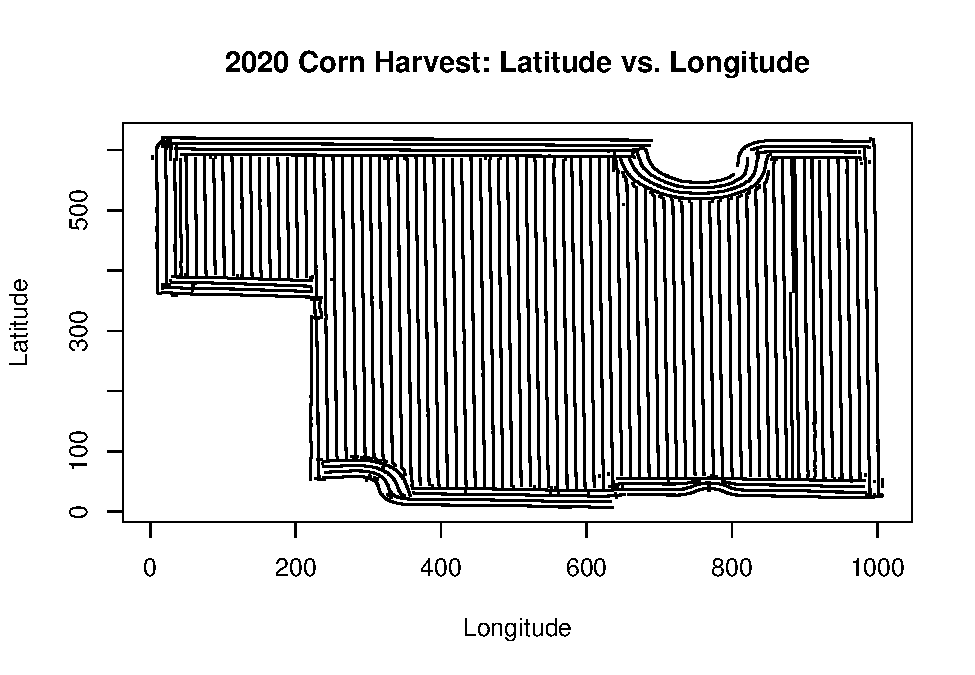
\includegraphics[keepaspectratio]{FinalProject2024X3_HR_files/figure-latex/raw-scatter-formula-1.pdf}}

\subsubsection{2. 2020 Harvest Spatial Grid Format (50m x
50m)}\label{harvest-spatial-grid-format-50m-x-50m}

\(dim=50mx50m\). \(Row as cal Lat\), \(Col as cal Long\) and
\(a \cdot \text{Lat} + b \cdot \text{Long}\) (cell a linear combination
of Lat and Long for cornHarvest 2020); Added abline included.

\begin{Shaded}
\begin{Highlighting}[]
\CommentTok{\# Assign grid positions}
\NormalTok{cornHarvest\_2020}\SpecialCharTok{$}\NormalTok{Row    }\OtherTok{\textless{}{-}} \FunctionTok{ceiling}\NormalTok{(cornHarvest\_2020}\SpecialCharTok{$}\NormalTok{Latitude }\SpecialCharTok{/} \DecValTok{50}\NormalTok{)}
\NormalTok{cornHarvest\_2020}\SpecialCharTok{$}\NormalTok{Column }\OtherTok{\textless{}{-}} \FunctionTok{ceiling}\NormalTok{(cornHarvest\_2020}\SpecialCharTok{$}\NormalTok{Longitude }\SpecialCharTok{/} \DecValTok{50}\NormalTok{)}
\NormalTok{cornHarvest\_2020}\SpecialCharTok{$}\NormalTok{Cell   }\OtherTok{\textless{}{-}}\NormalTok{ cornHarvest\_2020}\SpecialCharTok{$}\NormalTok{Row }\SpecialCharTok{*} \DecValTok{1000} \SpecialCharTok{+}\NormalTok{ cornHarvest\_2020}\SpecialCharTok{$}\NormalTok{Column}

\FunctionTok{plot}\NormalTok{(Latitude }\SpecialCharTok{\textasciitilde{}}\NormalTok{ Longitude, }\AttributeTok{data =}\NormalTok{ cornHarvest\_2020,}
     \AttributeTok{pch =} \StringTok{"."}\NormalTok{, }\AttributeTok{col =} \StringTok{"black"}\NormalTok{,}
     \AttributeTok{main =} \StringTok{"2020 Corn Harvest with 50x50m Grid"}\NormalTok{,}
     \AttributeTok{xlab =} \StringTok{"Longitude"}\NormalTok{, }\AttributeTok{ylab =} \StringTok{"Latitude"}\NormalTok{)}

\CommentTok{\# Add 50m{-}spaced grid lines}
\FunctionTok{abline}\NormalTok{(}\AttributeTok{h =} \DecValTok{1}\SpecialCharTok{:}\DecValTok{12} \SpecialCharTok{*} \DecValTok{50}\NormalTok{, }\AttributeTok{v =} \DecValTok{1}\SpecialCharTok{:}\DecValTok{20} \SpecialCharTok{*} \DecValTok{50}\NormalTok{, }\AttributeTok{col =} \StringTok{\textquotesingle{}red\textquotesingle{}}\NormalTok{)}
\end{Highlighting}
\end{Shaded}

\pandocbounded{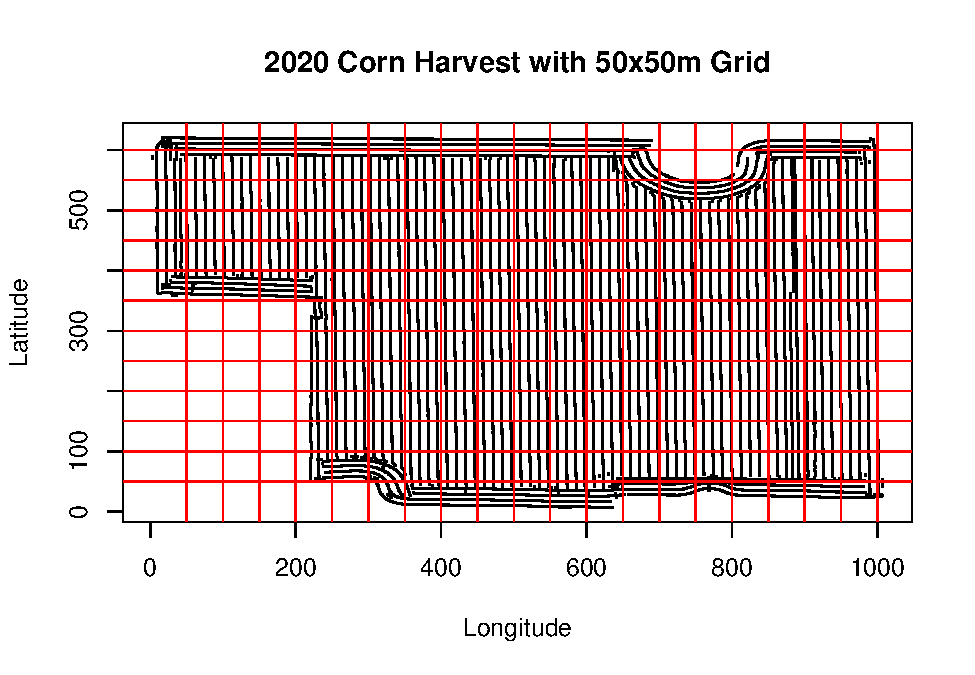
\includegraphics[keepaspectratio]{FinalProject2024X3_HR_files/figure-latex/raw-scatter-1.pdf}}

\textbf{Note:} This plot demonstrates the merging of data points
(Longitude, Latitude) to a single point (Cell) via use of mathematical
mapping. Along the journey, we note that there might also be times to
unravel the almagated `cell' to its original dimensions - \emph{Lon} and
\emph{Lat}. Further aggregation will later be done by computing the mean
and number of observation of each grid cell.

\subsubsection{3. HeatMap: 2020 Corn
Yield}\label{heatmap-2020-corn-yield}

\begin{Shaded}
\begin{Highlighting}[]
\CommentTok{\# Filter out rows where Y20 is NA}
\NormalTok{plot\_data }\OtherTok{\textless{}{-}}\NormalTok{ Combined.dat[}\SpecialCharTok{!}\FunctionTok{is.na}\NormalTok{(Combined.dat}\SpecialCharTok{$}\NormalTok{Y20), ]}

\CommentTok{\# Create color palette}
\NormalTok{num\_colors }\OtherTok{\textless{}{-}} \DecValTok{100}
\NormalTok{color\_bins }\OtherTok{\textless{}{-}} \FunctionTok{cut}\NormalTok{(plot\_data}\SpecialCharTok{$}\NormalTok{Y20, }\AttributeTok{breaks =}\NormalTok{ num\_colors)}
\NormalTok{colors }\OtherTok{\textless{}{-}} \FunctionTok{heat.colors}\NormalTok{(num\_colors)[}\FunctionTok{as.numeric}\NormalTok{(color\_bins)]}

\CommentTok{\# Plot colored grid cells}
\FunctionTok{plot}\NormalTok{(plot\_data}\SpecialCharTok{$}\NormalTok{Column, plot\_data}\SpecialCharTok{$}\NormalTok{Row,}
     \AttributeTok{col =}\NormalTok{ colors, }\AttributeTok{pch =} \DecValTok{15}\NormalTok{, }\AttributeTok{cex =} \FloatTok{1.5}\NormalTok{,}
     \AttributeTok{xlab =} \StringTok{"Grid Column"}\NormalTok{, }\AttributeTok{ylab =} \StringTok{"Grid Row"}\NormalTok{,}
     \AttributeTok{main =} \StringTok{"Heatmap of Y20 (2020 Corn Yield)"}\NormalTok{)}
\end{Highlighting}
\end{Shaded}

\pandocbounded{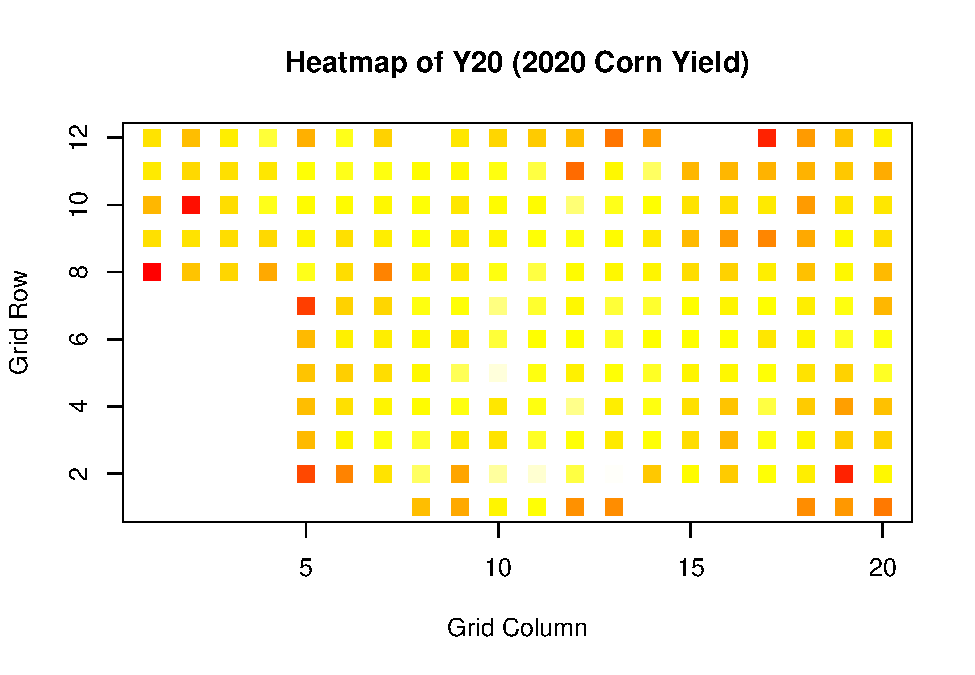
\includegraphics[keepaspectratio]{FinalProject2024X3_HR_files/figure-latex/heatmap-y20-1.pdf}}

\subsubsection{4. Combined Grid Layout Plot (Raw
Data)}\label{combined-grid-layout-plot-raw-data}

\begin{Shaded}
\begin{Highlighting}[]
\CommentTok{\# Visualize cell layout for all merged grid cells}
\FunctionTok{plot}\NormalTok{(Combined.dat}\SpecialCharTok{$}\NormalTok{Column, Combined.dat}\SpecialCharTok{$}\NormalTok{Row,}
     \AttributeTok{pch =} \DecValTok{15}\NormalTok{, }\AttributeTok{col =} \StringTok{"darkgreen"}\NormalTok{,}
     \AttributeTok{xlab =} \StringTok{"Grid Column"}\NormalTok{, }\AttributeTok{ylab =} \StringTok{"Grid Row"}\NormalTok{,}
     \AttributeTok{main =} \StringTok{"Grid Layout of Combined.dat"}\NormalTok{)}
\FunctionTok{abline}\NormalTok{(}\AttributeTok{h =} \DecValTok{1}\SpecialCharTok{:}\DecValTok{12} \SpecialCharTok{+} \FloatTok{0.5}\NormalTok{, }\AttributeTok{v =} \DecValTok{1}\SpecialCharTok{:}\DecValTok{20} \SpecialCharTok{+} \FloatTok{0.5}\NormalTok{, }\AttributeTok{col =} \StringTok{\textquotesingle{}red\textquotesingle{}}\NormalTok{)  }\CommentTok{\# grid lines}
\end{Highlighting}
\end{Shaded}

\pandocbounded{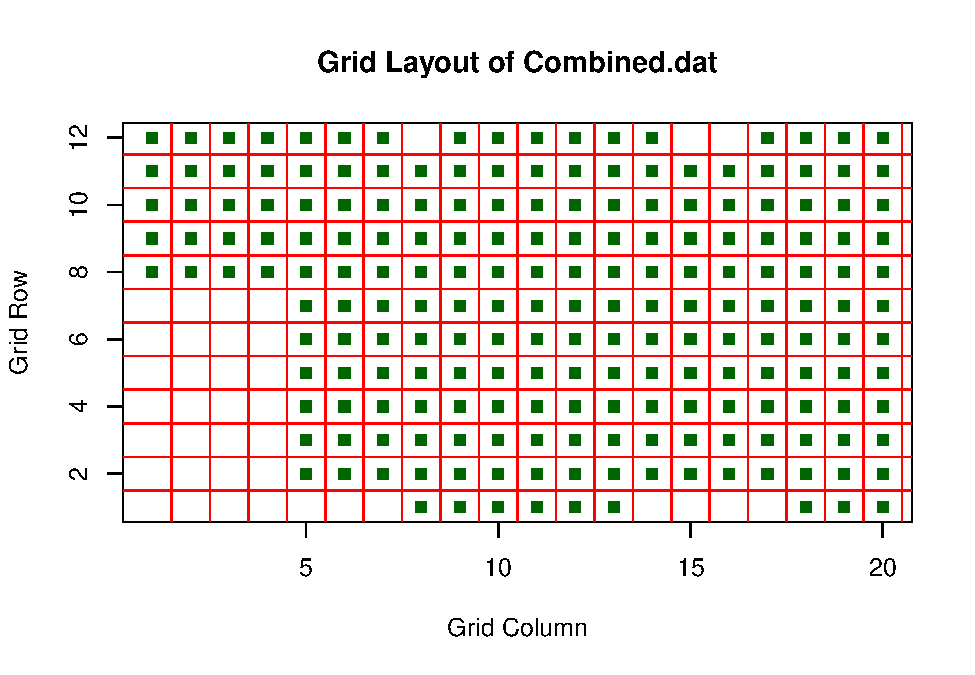
\includegraphics[keepaspectratio]{FinalProject2024X3_HR_files/figure-latex/grid-combined-plot-1.pdf}}

\begin{Shaded}
\begin{Highlighting}[]
\CommentTok{\#head(Combined.dat)}
\end{Highlighting}
\end{Shaded}

\textbf{Notes:} Further aggregation in the form of the number of
combined cells (with counts \textless= 30) is being used to produce this
merged plot.

\subsubsection{5. Visualized Pairs Plot}\label{visualized-pairs-plot}

Use a pairs plot to show the relationship among the data columns for the
combined data set.

\begin{Shaded}
\begin{Highlighting}[]
\CommentTok{\# Check variables exist and are complete enough}
\NormalTok{pairs\_vars }\OtherTok{\textless{}{-}} \FunctionTok{c}\NormalTok{(}\StringTok{"Y17"}\NormalTok{, }\StringTok{"AR18"}\NormalTok{, }\StringTok{"Y18"}\NormalTok{, }\StringTok{"Y19"}\NormalTok{, }\StringTok{"AR20"}\NormalTok{, }\StringTok{"Y20"}\NormalTok{)}

\CommentTok{\# Optional: remove rows with any NA values in those columns}
\NormalTok{Combined\_clean }\OtherTok{\textless{}{-}}\NormalTok{ Combined.dat[}\FunctionTok{complete.cases}\NormalTok{(Combined.dat[, pairs\_vars]), ]}

\CommentTok{\# Create the pairs plot}
\FunctionTok{pairs}\NormalTok{(Combined\_clean[, pairs\_vars],}
      \AttributeTok{main =} \StringTok{"Pairs Plot: Raw Aggregated Data"}\NormalTok{,}
      \AttributeTok{pch =} \DecValTok{21}\NormalTok{, }\AttributeTok{col =} \StringTok{"blue"}\NormalTok{, }\AttributeTok{cex.labels =} \FloatTok{1.1}\NormalTok{,}
      \AttributeTok{cex =} \FloatTok{0.8}\NormalTok{)}
\end{Highlighting}
\end{Shaded}

\pandocbounded{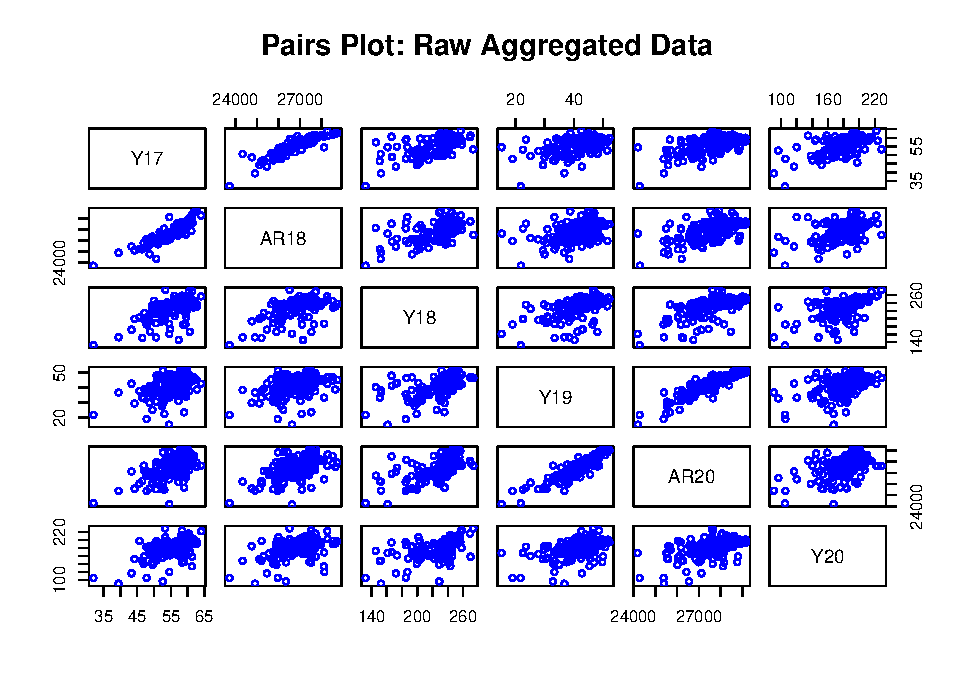
\includegraphics[keepaspectratio]{FinalProject2024X3_HR_files/figure-latex/pairs-raw-1.pdf}}

\textbf{Note:} Raw Data PAIR PLOT Noting that the Pairs Plot is a
symmetric diagram, we can use the lower triangular portion to access the
relations between variables given that the relation between \emph{a} and
\emph{b} is equivalent to the relation between \emph{b} and \emph{a}. We
hereby note that while a straight line can be fitted to most of the
ploted cases, only in two instances are there evidence of strong linear
correlations: between \(\text{AR18}\) and \(\text{Y17}\) \emph{and}
between \(\text{AR20}\) and \(\text{AR19}\).

\begin{Shaded}
\begin{Highlighting}[]
\FunctionTok{nrow}\NormalTok{(Combined\_clean)}
\end{Highlighting}
\end{Shaded}

\begin{verbatim}
## [1] 202
\end{verbatim}

\subsubsection{Prepare Combined RAW Dataset - Bayesian
Modeling}\label{prepare-combined-raw-dataset---bayesian-modeling}

We filter the dataset to keep only complete cases (no missing values)
across the six variables needed for the DAG models.

\begin{Shaded}
\begin{Highlighting}[]
\NormalTok{key\_vars }\OtherTok{\textless{}{-}} \FunctionTok{c}\NormalTok{(}\StringTok{"Y17"}\NormalTok{, }\StringTok{"AR18"}\NormalTok{, }\StringTok{"Y18"}\NormalTok{, }\StringTok{"Y19"}\NormalTok{, }\StringTok{"AR20"}\NormalTok{, }\StringTok{"Y20"}\NormalTok{)}

\CommentTok{\# Filter to complete cases}
\NormalTok{Combined.dat }\OtherTok{\textless{}{-}}\NormalTok{ Combined.dat[}\FunctionTok{complete.cases}\NormalTok{(Combined.dat[, key\_vars]), ]}

\CommentTok{\# Pre{-}checks to ensure formatting.  Define the key variable names}
\NormalTok{key\_vars }\OtherTok{\textless{}{-}} \FunctionTok{c}\NormalTok{(}\StringTok{"Y17"}\NormalTok{, }\StringTok{"AR18"}\NormalTok{, }\StringTok{"Y18"}\NormalTok{, }\StringTok{"Y19"}\NormalTok{, }\StringTok{"AR20"}\NormalTok{, }\StringTok{"Y20"}\NormalTok{)}

\CommentTok{\# Want data to be framed: dataframe format }
\ControlFlowTok{if}\NormalTok{ (}\SpecialCharTok{!}\FunctionTok{is.data.frame}\NormalTok{(Combined.dat)) \{}
  \FunctionTok{stop}\NormalTok{(}\StringTok{"Error: ‘Combined2’ is not a data.frame"}\NormalTok{)}
\NormalTok{\}}

\CommentTok{\# Check all key columns are present}
\NormalTok{missing\_vars }\OtherTok{\textless{}{-}} \FunctionTok{setdiff}\NormalTok{(key\_vars, }\FunctionTok{names}\NormalTok{(Combined.dat))}
\ControlFlowTok{if}\NormalTok{ (}\FunctionTok{length}\NormalTok{(missing\_vars) }\SpecialCharTok{\textgreater{}} \DecValTok{0}\NormalTok{) \{}
  \FunctionTok{stop}\NormalTok{(}\StringTok{"Error: Missing columns: "}\NormalTok{, }\FunctionTok{paste}\NormalTok{(missing\_vars, }\AttributeTok{collapse =} \StringTok{", "}\NormalTok{))}
\NormalTok{\}}

\CommentTok{\# Check each key column is numeric}
\ControlFlowTok{for}\NormalTok{ (v }\ControlFlowTok{in}\NormalTok{ key\_vars) \{}
  \ControlFlowTok{if}\NormalTok{ (}\SpecialCharTok{!}\FunctionTok{is.numeric}\NormalTok{(Combined.dat[[v]])) \{}
    \FunctionTok{stop}\NormalTok{(}\StringTok{"Error: Column ‘"}\NormalTok{, v, }\StringTok{"’ is not numeric"}\NormalTok{)}
\NormalTok{  \}}
\NormalTok{\}}

\CommentTok{\# Remove any rows with NAs in their columns}
\NormalTok{Combined2 }\OtherTok{\textless{}{-}}\NormalTok{ Combined.dat[}\FunctionTok{complete.cases}\NormalTok{(Combined.dat[, key\_vars]), ]}
\end{Highlighting}
\end{Shaded}

\begin{Shaded}
\begin{Highlighting}[]
\CommentTok{\#head(Combined2)}
\FunctionTok{nrow}\NormalTok{(Combined2)}
\end{Highlighting}
\end{Shaded}

\begin{verbatim}
## [1] 202
\end{verbatim}

\begin{Shaded}
\begin{Highlighting}[]
\CommentTok{\#nrow(Combined.dat)}
\end{Highlighting}
\end{Shaded}

\subsubsection{6. Causal Analysis - DAG for RAW
Dataset}\label{causal-analysis---dag-for-raw-dataset}

\subsubsection{i. DAG model for 2017 -
2018}\label{i.-dag-model-for-2017---2018}

\begin{Shaded}
\begin{Highlighting}[]
\FunctionTok{library}\NormalTok{(bnlearn)}
\end{Highlighting}
\end{Shaded}

\begin{verbatim}
## Warning: package 'bnlearn' was built under R version 4.5.1
\end{verbatim}

\begin{Shaded}
\begin{Highlighting}[]
\FunctionTok{library}\NormalTok{(Rgraphviz)}
\end{Highlighting}
\end{Shaded}

\begin{verbatim}
## Loading required package: graph
\end{verbatim}

\begin{verbatim}
## Loading required package: BiocGenerics
\end{verbatim}

\begin{verbatim}
## Loading required package: generics
\end{verbatim}

\begin{verbatim}
## Warning: package 'generics' was built under R version 4.5.1
\end{verbatim}

\begin{verbatim}
## 
## Attaching package: 'generics'
\end{verbatim}

\begin{verbatim}
## The following objects are masked from 'package:base':
## 
##     as.difftime, as.factor, as.ordered, intersect, is.element, setdiff,
##     setequal, union
\end{verbatim}

\begin{verbatim}
## 
## Attaching package: 'BiocGenerics'
\end{verbatim}

\begin{verbatim}
## The following object is masked from 'package:bnlearn':
## 
##     score
\end{verbatim}

\begin{verbatim}
## The following objects are masked from 'package:stats':
## 
##     IQR, mad, sd, var, xtabs
\end{verbatim}

\begin{verbatim}
## The following objects are masked from 'package:base':
## 
##     anyDuplicated, aperm, append, as.data.frame, basename, cbind,
##     colnames, dirname, do.call, duplicated, eval, evalq, Filter, Find,
##     get, grep, grepl, is.unsorted, lapply, Map, mapply, match, mget,
##     order, paste, pmax, pmax.int, pmin, pmin.int, Position, rank,
##     rbind, Reduce, rownames, sapply, saveRDS, table, tapply, unique,
##     unsplit, which.max, which.min
\end{verbatim}

\begin{verbatim}
## 
## Attaching package: 'graph'
\end{verbatim}

\begin{verbatim}
## The following objects are masked from 'package:bnlearn':
## 
##     degree, nodes, nodes<-
\end{verbatim}

\begin{verbatim}
## Loading required package: grid
\end{verbatim}

\begin{Shaded}
\begin{Highlighting}[]
\NormalTok{modela.dag }\OtherTok{\textless{}{-}} \FunctionTok{model2network}\NormalTok{(}\StringTok{"[Y17][AR18|Y17][Y18|AR18:Y17]"}\NormalTok{)}
\NormalTok{fit1 }\OtherTok{=} \FunctionTok{bn.fit}\NormalTok{(modela.dag, Combined2[,}\FunctionTok{c}\NormalTok{(}\StringTok{\textquotesingle{}Y17\textquotesingle{}}\NormalTok{,}\StringTok{\textquotesingle{}AR18\textquotesingle{}}\NormalTok{,}\StringTok{\textquotesingle{}Y18\textquotesingle{}}\NormalTok{)])}

\CommentTok{\# fit1}
\NormalTok{strengtha }\OtherTok{\textless{}{-}} \FunctionTok{arc.strength}\NormalTok{(modela.dag, Combined2[,}\FunctionTok{c}\NormalTok{(}\StringTok{\textquotesingle{}Y17\textquotesingle{}}\NormalTok{,}\StringTok{\textquotesingle{}AR18\textquotesingle{}}\NormalTok{,}\StringTok{\textquotesingle{}Y18\textquotesingle{}}\NormalTok{)])}
\FunctionTok{strength.plot}\NormalTok{(modela.dag, strengtha)}
\end{Highlighting}
\end{Shaded}

\pandocbounded{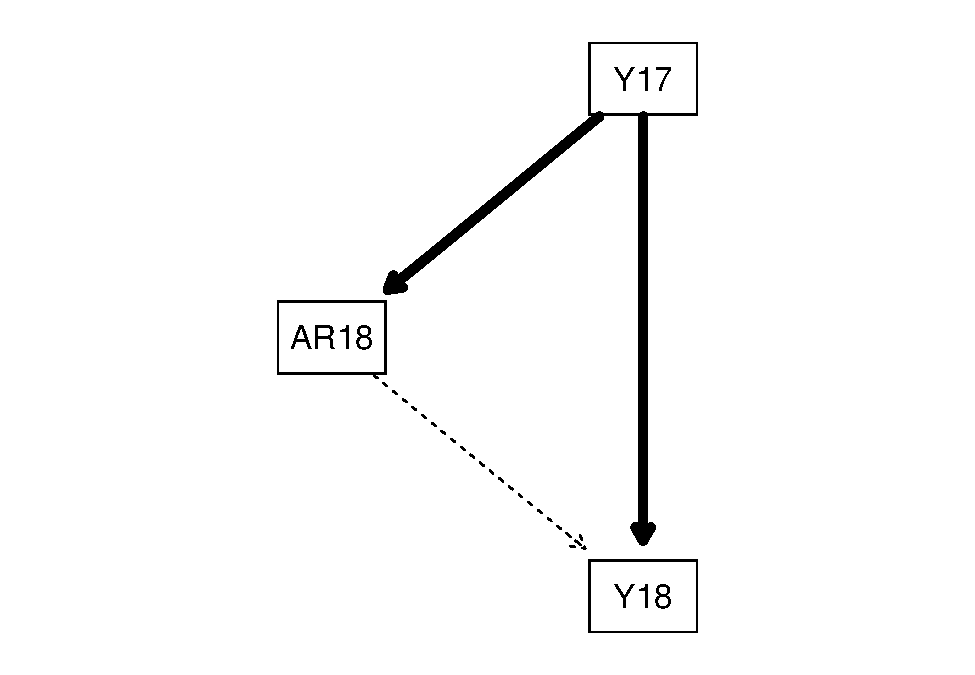
\includegraphics[keepaspectratio]{FinalProject2024X3_HR_files/figure-latex/combDtaDirGraph_2017-1.pdf}}

\subsubsection{Interpretation of DAG model: 2017 -
2018}\label{interpretation-of-dag-model-2017---2018}

\textbf{The yield of 2017 is a strong predictor for both the 2018
Applied Rate and 2017 yield but the applied rate of 2018 (AP18) is not a
strong support for the same year's yield (Y18). Reference to the latter
point, needs further investigation. Arising questions can be: was there
measurement error, insufficient data, or collinearity (overlapping or
redundant information between Y17 and AR18)? }

\subsubsection{ii. DAG model for 2019 -
2020}\label{ii.-dag-model-for-2019---2020}

\begin{Shaded}
\begin{Highlighting}[]
\FunctionTok{library}\NormalTok{(bnlearn)}
\FunctionTok{library}\NormalTok{(Rgraphviz)}

\NormalTok{modelb.dag }\OtherTok{\textless{}{-}} \FunctionTok{model2network}\NormalTok{(}\StringTok{"[Y19][AR20|Y19][Y20|AR20:Y19]"}\NormalTok{)}
\NormalTok{fit2 }\OtherTok{=} \FunctionTok{bn.fit}\NormalTok{(modelb.dag, Combined2[,}\FunctionTok{c}\NormalTok{(}\StringTok{\textquotesingle{}Y19\textquotesingle{}}\NormalTok{,}\StringTok{\textquotesingle{}AR20\textquotesingle{}}\NormalTok{,}\StringTok{\textquotesingle{}Y20\textquotesingle{}}\NormalTok{)])}
\CommentTok{\#fit2}
\NormalTok{strengthb }\OtherTok{\textless{}{-}} \FunctionTok{arc.strength}\NormalTok{(modelb.dag, Combined2[,}\FunctionTok{c}\NormalTok{(}\StringTok{\textquotesingle{}Y19\textquotesingle{}}\NormalTok{,}\StringTok{\textquotesingle{}AR20\textquotesingle{}}\NormalTok{,}\StringTok{\textquotesingle{}Y20\textquotesingle{}}\NormalTok{)])}
\FunctionTok{strength.plot}\NormalTok{(modelb.dag, strengthb)}
\end{Highlighting}
\end{Shaded}

\pandocbounded{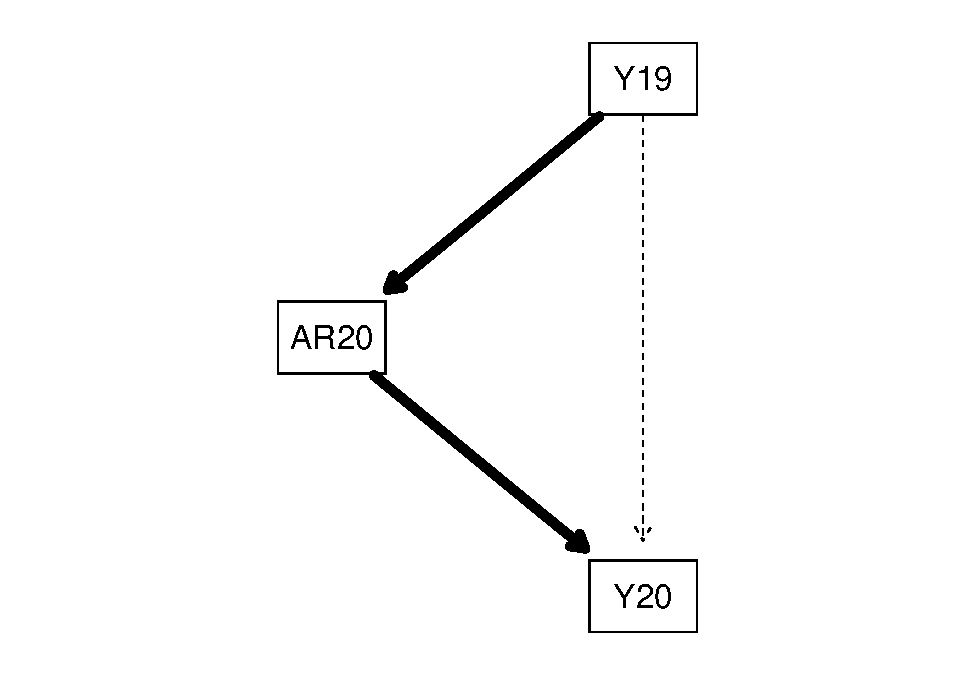
\includegraphics[keepaspectratio]{FinalProject2024X3_HR_files/figure-latex/combDtaDirGraph_2019-1.pdf}}

\subsubsection{Interpretation of the DAG model 2019 -
2020}\label{interpretation-of-the-dag-model-2019---2020}

The yield of 2019 is a strong predictor for both the Applied Rate of
2020 which itself has a strong influence on the 2020 yield. That is, the
yield of 2019 has a indirect consequence on the 2020 yield. We can
therefore conclude that current seeding rate (AR20) and current-year
factors (Y20) are tightly linked---likely due to mutual determination or
shared causality under the current circumstances.

\subsubsection{iii. DAG model for ALL Years: 2017 -
2020}\label{iii.-dag-model-for-all-years-2017---2020}

\begin{Shaded}
\begin{Highlighting}[]
\FunctionTok{library}\NormalTok{(bnlearn)}
\FunctionTok{library}\NormalTok{(Rgraphviz)}

\NormalTok{modela.dag }\OtherTok{\textless{}{-}} \FunctionTok{model2network}\NormalTok{(}\StringTok{"[Y17][AR18|Y17][Y18|AR18:Y17]"}\NormalTok{)}
\NormalTok{fita }\OtherTok{=} \FunctionTok{bn.fit}\NormalTok{(modela.dag, Combined2[,}\FunctionTok{c}\NormalTok{(}\StringTok{\textquotesingle{}Y17\textquotesingle{}}\NormalTok{,}\StringTok{\textquotesingle{}AR18\textquotesingle{}}\NormalTok{,}\StringTok{\textquotesingle{}Y18\textquotesingle{}}\NormalTok{)])}

\NormalTok{strengtha }\OtherTok{\textless{}{-}} \FunctionTok{arc.strength}\NormalTok{(modela.dag, Combined2[,}\FunctionTok{c}\NormalTok{(}\StringTok{\textquotesingle{}Y17\textquotesingle{}}\NormalTok{,}\StringTok{\textquotesingle{}AR18\textquotesingle{}}\NormalTok{,}\StringTok{\textquotesingle{}Y18\textquotesingle{}}\NormalTok{)])}
\CommentTok{\#strength.plot(modela.dag, strengtha)}

\NormalTok{modelb.dag }\OtherTok{\textless{}{-}} \FunctionTok{model2network}\NormalTok{(}\StringTok{"[Y19][AR20|Y19][Y20|AR20:Y19]"}\NormalTok{)}
\NormalTok{fitv }\OtherTok{=} \FunctionTok{bn.fit}\NormalTok{(modelb.dag, Combined2[,}\FunctionTok{c}\NormalTok{(}\StringTok{\textquotesingle{}Y19\textquotesingle{}}\NormalTok{,}\StringTok{\textquotesingle{}AR20\textquotesingle{}}\NormalTok{,}\StringTok{\textquotesingle{}Y20\textquotesingle{}}\NormalTok{)])}

\NormalTok{strengthb }\OtherTok{\textless{}{-}} \FunctionTok{arc.strength}\NormalTok{(modelb.dag, Combined2[,}\FunctionTok{c}\NormalTok{(}\StringTok{\textquotesingle{}Y19\textquotesingle{}}\NormalTok{,}\StringTok{\textquotesingle{}AR20\textquotesingle{}}\NormalTok{,}\StringTok{\textquotesingle{}Y20\textquotesingle{}}\NormalTok{)])}
\CommentTok{\#strength.plot(modelb.dag, strengthb)}

\NormalTok{modelc.dag }\OtherTok{\textless{}{-}} \FunctionTok{model2network}\NormalTok{(}\StringTok{"[Y17][AR18|Y17][Y18|AR18:Y17][Y19|Y17:AR18:Y18][AR20|Y19][Y20|AR20:Y19]"}\NormalTok{)}
\NormalTok{fitc }\OtherTok{=} \FunctionTok{bn.fit}\NormalTok{(modelc.dag, Combined2[,}\FunctionTok{c}\NormalTok{(}\StringTok{\textquotesingle{}Y17\textquotesingle{}}\NormalTok{,}\StringTok{\textquotesingle{}AR18\textquotesingle{}}\NormalTok{,}\StringTok{\textquotesingle{}Y18\textquotesingle{}}\NormalTok{,}\StringTok{\textquotesingle{}Y19\textquotesingle{}}\NormalTok{,}\StringTok{\textquotesingle{}AR20\textquotesingle{}}\NormalTok{,}\StringTok{\textquotesingle{}Y20\textquotesingle{}}\NormalTok{)])}

\NormalTok{strengthc }\OtherTok{\textless{}{-}} \FunctionTok{arc.strength}\NormalTok{(modelc.dag, Combined2[,}\FunctionTok{c}\NormalTok{(}\StringTok{\textquotesingle{}Y17\textquotesingle{}}\NormalTok{,}\StringTok{\textquotesingle{}AR18\textquotesingle{}}\NormalTok{,}\StringTok{\textquotesingle{}Y18\textquotesingle{}}\NormalTok{,}\StringTok{\textquotesingle{}Y19\textquotesingle{}}\NormalTok{,}\StringTok{\textquotesingle{}AR20\textquotesingle{}}\NormalTok{,}\StringTok{\textquotesingle{}Y20\textquotesingle{}}\NormalTok{)])}
\FunctionTok{strength.plot}\NormalTok{(modelc.dag, strengthc)}
\end{Highlighting}
\end{Shaded}

\pandocbounded{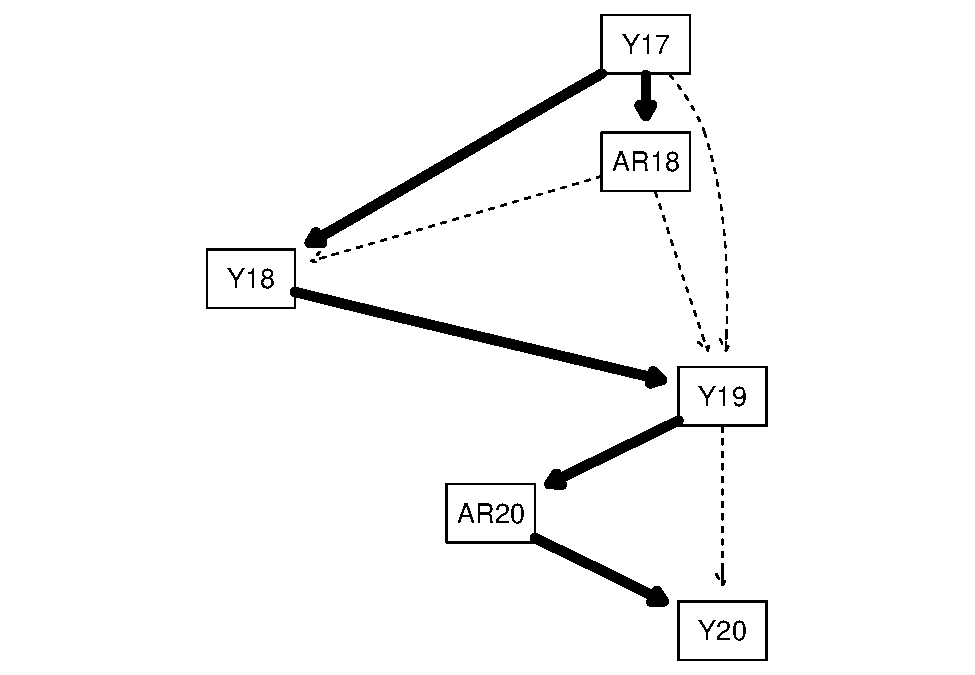
\includegraphics[keepaspectratio]{FinalProject2024X3_HR_files/figure-latex/combDtaDirGraph_17_20-1.pdf}}

\paragraph{Interpretation of the 2017-2020 DAG
model:}\label{interpretation-of-the-2017-2020-dag-model}

\textbf{Notes:} - In short the effect of Y17 on Y20 follows this path:
\(Y17 \rightarrow Y18 \rightarrow Y19 \rightarrow AR20 \rightarrow Y20\).

\begin{itemize}
\item
  We note though that has an indirect effect on Y20 and begs a question
  that Y19 impacts Y20 via some intervening management decision, not
  necessarily a direct soil or environmental one.
\item
  Also the yield of 2017 has a strong bearing also on the applied rate
  for 2018. Here again, Y17 is prominent.
\item
  Further, we note that the graph is acyclic which is a requirement of
  Bayesian Models.
\end{itemize}

\subsubsection{7. Calculated Strengths of DAG: 2017-2020 RAW
Data}\label{calculated-strengths-of-dag-2017-2020-raw-data}

\begin{Shaded}
\begin{Highlighting}[]
\FunctionTok{library}\NormalTok{(bnlearn)}

\CommentTok{\# Learn the network structure}
\NormalTok{modelc.dag }\OtherTok{\textless{}{-}} \FunctionTok{hc}\NormalTok{(Combined2)  }\CommentTok{\# Can be replaced by other tests:gs(), tabu()}

\CommentTok{\# Compute arc strength values using test{-}based criterion}
\NormalTok{strength\_df }\OtherTok{\textless{}{-}} \FunctionTok{arc.strength}\NormalTok{(modelc.dag, }\AttributeTok{data =}\NormalTok{ Combined2, }\AttributeTok{criterion =} \StringTok{"cor"}\NormalTok{)}

\CommentTok{\# View the first few rows}
\FunctionTok{head}\NormalTok{(strength\_df)}
\end{Highlighting}
\end{Shaded}

\begin{verbatim}
##   from   to     strength
## 1 Cell  Row 0.000000e+00
## 2  Y19 AR20 4.345973e-84
## 3  Y17 AR18 6.864785e-75
## 4 AR20  Y18 5.787313e-27
## 5  Y18  Y17 3.450074e-08
## 6  Y17  Y20 2.184471e-07
\end{verbatim}

\textbf{Note:} While similar analysis can be done for previously
generated plot, we focus here on the all inclusive plot for the 4 year
period. The arc from \(\texttt{Y19 → AR20}\) ; (p \approx 4.3
\times 10\^{}\{-84\}) exhibits the strongest statistical connection
among all variables, suggesting a highly reliable directional
dependency. Similarly, the link \{Y17\}
\(\rightarrow \mathrm {AR18} \ (p \approx 6.9 \times 10^{-75})\) is
backed by extremely strong evidence. Though all connections are
statistically significant (p \textless{} 0.001), the strength
progressively weakens down the list, with the Y17 → Y20 link being the
least strong yet notable with (p ≈ 2.2e-07).

\begin{Shaded}
\begin{Highlighting}[]
\CommentTok{\# Sort the strengths}
\NormalTok{sorted\_strengths }\OtherTok{\textless{}{-}}\NormalTok{ strength\_df[}\FunctionTok{order}\NormalTok{(}\SpecialCharTok{{-}}\NormalTok{strength\_df}\SpecialCharTok{$}\NormalTok{strength), ]}

\NormalTok{sorted\_strengths}
\end{Highlighting}
\end{Shaded}

\begin{verbatim}
##      from     to     strength
## 15 Column   Cell 8.838431e-03
## 14    Y19    Y20 7.530096e-03
## 13    Y20 Column 6.799116e-03
## 12    Y20    Row 5.928840e-03
## 11   AR18    Y20 3.900722e-03
## 8     Y18    Y20 3.370811e-04
## 10    Y17    Row 4.871457e-05
## 9     Y17 Column 2.803416e-05
## 7    AR20    Y17 7.030443e-07
## 6     Y17    Y20 2.184471e-07
## 5     Y18    Y17 3.450074e-08
## 4    AR20    Y18 5.787313e-27
## 3     Y17   AR18 6.864785e-75
## 2     Y19   AR20 4.345973e-84
## 1    Cell    Row 0.000000e+00
\end{verbatim}

\subsubsection{8. Visual Merged Raw
Dataset}\label{visual-merged-raw-dataset}

\begin{Shaded}
\begin{Highlighting}[]
\FunctionTok{head}\NormalTok{(Combined2)}
\end{Highlighting}
\end{Shaded}

\begin{verbatim}
##    Cell Row Column      Y17     AR18      Y18      Y19     AR20       Y20
## 1 10001  10      1 53.36685 26092.36 211.7009 39.14806 26885.62 165.10126
## 2 10002  10      2 52.58359 26339.74 228.9304 32.78266 26549.57  96.65559
## 3 10003  10      3 54.19551 26447.59 232.2385 37.58834 26845.56 179.71318
## 4 10004  10      4 50.76123 25925.29 237.7755 48.18398 27982.25 197.49239
## 5 10005  10      5 52.61351 25973.53 231.6592 51.50722 28824.57 192.00151
## 6 10006  10      6 54.95515 26260.49 238.1637 49.17503 28857.66 191.52483
\end{verbatim}

\begin{Shaded}
\begin{Highlighting}[]
\CommentTok{\#headc(Combined2)}
\FunctionTok{nrow}\NormalTok{(Combined.dat)}
\end{Highlighting}
\end{Shaded}

\begin{verbatim}
## [1] 202
\end{verbatim}

\section{G. PRE-NORMALIZATION
JUSTIFICATION}\label{g.-pre-normalization-justification}

To set the stage for normalization, we will show that the scaled raw
dataset, \emph{scalComb3}, contains an inordinate amount of outliers
which persists even when scaled. Outliers are data points falling
outside the +/- 3 standard deviation range.

\subsubsection{1. Outlier: Raw Combined
Dataset}\label{outlier-raw-combined-dataset}

\begin{Shaded}
\begin{Highlighting}[]
\NormalTok{vars }\OtherTok{\textless{}{-}} \FunctionTok{c}\NormalTok{(}\StringTok{"Y17"}\NormalTok{, }\StringTok{"AR18"}\NormalTok{, }\StringTok{"Y18"}\NormalTok{, }\StringTok{"Y19"}\NormalTok{, }\StringTok{"AR20"}\NormalTok{, }\StringTok{"Y20"}\NormalTok{)}

\CommentTok{\# Drop rows with missing values in selected columns}
\NormalTok{Combined3 }\OtherTok{\textless{}{-}}\NormalTok{ Combined2[}\FunctionTok{complete.cases}\NormalTok{(Combined2[, vars]), vars]}

\CommentTok{\# Compute Z{-}scores for cleaned data}
\NormalTok{z\_rawComb3 }\OtherTok{\textless{}{-}} \FunctionTok{scale}\NormalTok{(Combined3)}

\CommentTok{\# Flag outliers: values with |z| \textgreater{} 3}
\NormalTok{outlier\_Comb3 }\OtherTok{\textless{}{-}} \FunctionTok{abs}\NormalTok{(}\FunctionTok{scale}\NormalTok{(Combined3))}\SpecialCharTok{\textgreater{}}\DecValTok{3}

\CommentTok{\# Count of outliers per variable}
\FunctionTok{colSums}\NormalTok{(outlier\_Comb3)}
\end{Highlighting}
\end{Shaded}

\begin{verbatim}
##  Y17 AR18  Y18  Y19 AR20  Y20 
##    2    2    5    4    2    5
\end{verbatim}

\begin{Shaded}
\begin{Highlighting}[]
\CommentTok{\#head(Combined3)}
\FunctionTok{nrow}\NormalTok{(Combined3)}
\end{Highlighting}
\end{Shaded}

\begin{verbatim}
## [1] 202
\end{verbatim}

\textbf{Outlier Analysis:} - Outliers are present across all years
ranging from 2 to 5

\begin{itemize}
\item
  Y18 and Y20 (corn harvests yields) have the highest number of
  outliers, suggesting either possible variability in corn yields
  perhaps due to unusual environmental conditions or sensor error in
  these years.
\item
  AR18 and AR20 (applied rates), have a lower cases of outliers,
  possibly due to machine adjustability, soil viability, or even the
  effect of fields' edges.
\item
  From the data, we can conclude that the yield rates after 2017 show
  increased variations in outliers.
\end{itemize}

\subsubsection{2. Boxplot: Raw Combined
Data}\label{boxplot-raw-combined-data}

\begin{Shaded}
\begin{Highlighting}[]
\CommentTok{\# Set layout: 1 row, 2 plots}
\FunctionTok{par}\NormalTok{(}\AttributeTok{mfrow =} \FunctionTok{c}\NormalTok{(}\DecValTok{1}\NormalTok{, }\DecValTok{2}\NormalTok{))}

\CommentTok{\# Boxplot of raw values}
\FunctionTok{boxplot}\NormalTok{(Combined3,}
        \AttributeTok{main =} \StringTok{"Boxplot of Raw Values"}\NormalTok{,}
        \AttributeTok{ylab =} \StringTok{"Original Scale"}\NormalTok{,}
        \AttributeTok{col =} \StringTok{"lightblue"}\NormalTok{,}
        \AttributeTok{outline =} \ConstantTok{TRUE}\NormalTok{,}
        \AttributeTok{las =} \DecValTok{2}\NormalTok{)}

\CommentTok{\# Boxplot of standardized values (z{-}scores)}
\FunctionTok{boxplot}\NormalTok{(outlier\_Comb3,}
        \AttributeTok{main =} \StringTok{"Boxplot of Z{-}scores"}\NormalTok{,}
        \AttributeTok{ylab =} \StringTok{"Z{-}score"}\NormalTok{,}
        \AttributeTok{col =} \StringTok{"lightgreen"}\NormalTok{,}
        \AttributeTok{outline =} \ConstantTok{TRUE}\NormalTok{,}
        \AttributeTok{las =} \DecValTok{2}\NormalTok{)}
\FunctionTok{abline}\NormalTok{(}\AttributeTok{h =} \FunctionTok{c}\NormalTok{(}\SpecialCharTok{{-}}\DecValTok{3}\NormalTok{, }\DecValTok{3}\NormalTok{), }\AttributeTok{col =} \StringTok{"red"}\NormalTok{, }\AttributeTok{lty =} \DecValTok{2}\NormalTok{)}
\end{Highlighting}
\end{Shaded}

\pandocbounded{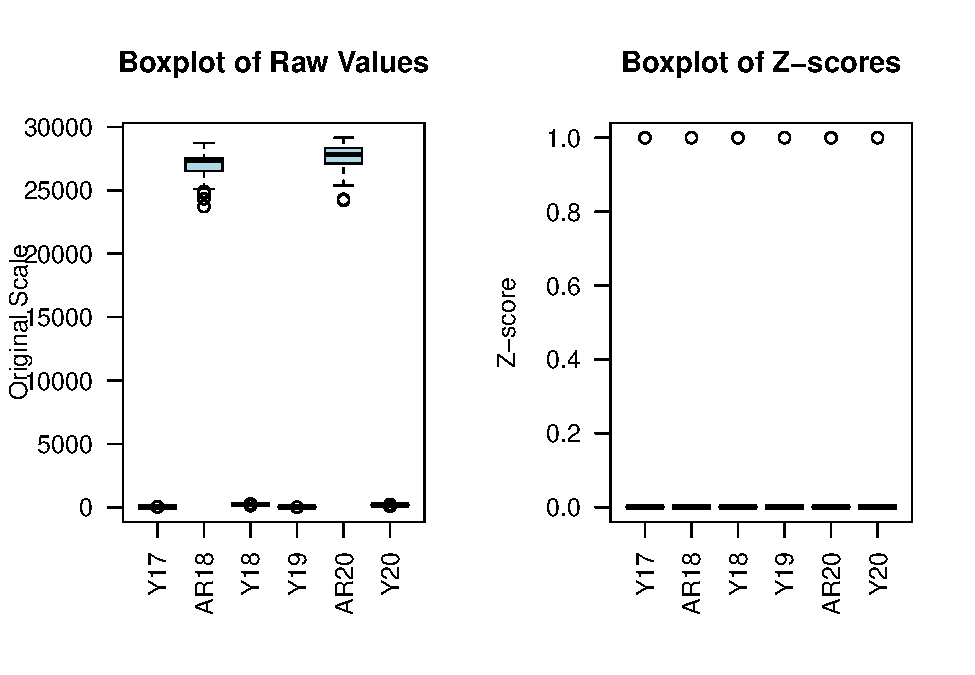
\includegraphics[keepaspectratio]{FinalProject2024X3_HR_files/figure-latex/unnamed-chunk-8-1.pdf}}

\begin{Shaded}
\begin{Highlighting}[]
\CommentTok{\# Reset layout}
\FunctionTok{par}\NormalTok{(}\AttributeTok{mfrow =} \FunctionTok{c}\NormalTok{(}\DecValTok{1}\NormalTok{, }\DecValTok{1}\NormalTok{))}
\end{Highlighting}
\end{Shaded}

\subsubsection{Boxplots Analysis:}\label{boxplots-analysis}

\textbf{Raw Dataset Boxplot:}

\begin{itemize}
\item
  Shows each variable in its real unit scale; hence the shown results -
  with the \emph{AppliedRate} variable way above the \emph{Yield}
  variable.
\item
  The Median AppliedRate is around \(27,500\) for Y18 and Y20 while all
  the yield variable appear with medians around 0.
\item
  Whiskers and outliers depend on the spread of raw values.
\item
  Care has to be taken in attempts to make comparison between the spread
  of these variables (AR and Y) since they are measured in different
  units and reference different crops
\end{itemize}

\textbf{Scaled Data Analysis:} - Standardizes all variables to mean = 0
and SD = 1.

\begin{itemize}
\item
  Helps detect which variables have extreme standardized deviations
  (\textbar z\textbar{} \textgreater{} 3).
\item
  The outlier threshold, which are usually shown by Red dashed lines are
  invisible here.
\end{itemize}

\subsubsection{3. Calculated Means, SD for Raw
Data}\label{calculated-means-sd-for-raw-data}

\begin{Shaded}
\begin{Highlighting}[]
\CommentTok{\# Define variable names}
\NormalTok{vars }\OtherTok{\textless{}{-}} \FunctionTok{c}\NormalTok{(}\StringTok{"Y17"}\NormalTok{, }\StringTok{"AR18"}\NormalTok{, }\StringTok{"Y18"}\NormalTok{, }\StringTok{"Y19"}\NormalTok{, }\StringTok{"AR20"}\NormalTok{, }\StringTok{"Y20"}\NormalTok{)}

\CommentTok{\# Calculate column means and standard deviations after normalization}
\NormalTok{norm\_means }\OtherTok{\textless{}{-}} \FunctionTok{colMeans}\NormalTok{(Combined3[, vars], }\AttributeTok{na.rm =} \ConstantTok{TRUE}\NormalTok{)}
\NormalTok{norm\_sds   }\OtherTok{\textless{}{-}} \FunctionTok{apply}\NormalTok{(Combined3[, vars], }\DecValTok{2}\NormalTok{, sd, }\AttributeTok{na.rm =} \ConstantTok{TRUE}\NormalTok{)}

\CommentTok{\# View resulting dataframe set of values}
\FunctionTok{data.frame}\NormalTok{(}\AttributeTok{Mean =} \FunctionTok{round}\NormalTok{(norm\_means, }\DecValTok{3}\NormalTok{), }\AttributeTok{SD =} \FunctionTok{round}\NormalTok{(norm\_sds, }\DecValTok{3}\NormalTok{))}
\end{Highlighting}
\end{Shaded}

\begin{verbatim}
##           Mean      SD
## Y17     56.328   4.441
## AR18 26995.999 807.019
## Y18    231.198  23.576
## Y19     42.473   6.362
## AR20 27656.972 938.077
## Y20    181.521  20.992
\end{verbatim}

\emph{Notes}: This result gives a baseline snapshot of the raw dataset
--- the average values and their variability for each yield and applied
rate over the years. It allows for comparison of the magnitude and
spread of different variables before any transformation, helping guide
normalization and modeling steps. When the data is transformed,
\(\mu \approx 0\) and \(\sigma \approx 1\)

\subsubsection{Calculated Means, SD for Scaled
Data}\label{calculated-means-sd-for-scaled-data}

\begin{Shaded}
\begin{Highlighting}[]
\CommentTok{\# Define variable names}
\NormalTok{vars }\OtherTok{\textless{}{-}} \FunctionTok{c}\NormalTok{(}\StringTok{"Y17"}\NormalTok{, }\StringTok{"AR18"}\NormalTok{, }\StringTok{"Y18"}\NormalTok{, }\StringTok{"Y19"}\NormalTok{, }\StringTok{"AR20"}\NormalTok{, }\StringTok{"Y20"}\NormalTok{)}

\CommentTok{\# Calculate column means and standard deviations after normalization}
\NormalTok{norm\_means }\OtherTok{\textless{}{-}} \FunctionTok{colMeans}\NormalTok{(z\_rawComb3[, vars], }\AttributeTok{na.rm =} \ConstantTok{TRUE}\NormalTok{)}
\NormalTok{norm\_sds   }\OtherTok{\textless{}{-}} \FunctionTok{apply}\NormalTok{(z\_rawComb3[, vars], }\DecValTok{2}\NormalTok{, sd, }\AttributeTok{na.rm =} \ConstantTok{TRUE}\NormalTok{)}

\CommentTok{\# View resulting dataframe set of values}
\FunctionTok{data.frame}\NormalTok{(}\AttributeTok{Mean =} \FunctionTok{round}\NormalTok{(norm\_means, }\DecValTok{3}\NormalTok{), }\AttributeTok{SD =} \FunctionTok{round}\NormalTok{(norm\_sds, }\DecValTok{3}\NormalTok{))}
\end{Highlighting}
\end{Shaded}

\begin{verbatim}
##      Mean SD
## Y17     0  1
## AR18    0  1
## Y18     0  1
## Y19     0  1
## AR20    0  1
## Y20     0  1
\end{verbatim}

\subsubsection{Comparison Discussion Outliers of Combined Raw dataset vs
Combined Normalized
dataset:}\label{comparison-discussion-outliers-of-combined-raw-dataset-vs-combined-normalized-dataset}

\begin{itemize}
\tightlist
\item
  Which variables had many extreme values in raw or normalized form?
\end{itemize}

\textbf{NORMALIZED DATA:} - All scaled variables \textgreater{}
\(3\sigma\) - outside the range \((\mu - 3\sigma, \mu+3\sigma)\)

\begin{itemize}
\tightlist
\item
  Effect of Normalization: Following normalization, all variables in the
  dataset show means close to zero and standard deviations near one.
  Boxplot visualizations confirm that each distribution has been
  centered and rescaled appropriately, enabling cross-variable
  comparisons and minimizing the influence of scale/unit disparities.
\end{itemize}

\section{2. NORMALIZED DATA ANALYSIS}\label{normalized-data-analysis}

\section{A. Normalization Process}\label{a.-normalization-process}

To accomplish analysis on the same dataset, the same sequence of
processing performed (file read, count requirement (\textgreater=30),
calculaltion of mean \& stand deviation), and plotting) on the raw
dataset will be used here. Additionally, a method, referred to as the
Winsorize method will be employed prior to the common method of
normalizaling the data so that statistidal expedience could be brought
to the process. Winsorization, is the process of trimming extreme tail
values off datasets.

The data files contain three different measurement units for the data.
Files \texttt{2017\ Soybeans\ Harvest.csv} and
\texttt{2019\ Soybeans\ Harvest.csv} are soybean harvests datasets with
around 60 bu/acre. \texttt{2018\ Corn\ Harvest.csv} and
\texttt{2020\ Corn\ Harvest.csv} are corn harvests files with around 180
bu/acre, while \texttt{2018\ Corn\ Seeding.csv} and
\texttt{2020\ Corn\ Seeding.csv} contain seeding rate data. Given that
we are handling different crops, for different years, measuring in
different units for different field locations, normalization is
therefore required for a leveled analysis and to manage (lessen) lurking
outliers. With the in-hand datasets, we will examine the distribution
for outliers by comparing them for both the raw and normalized data by
visualizing boxplots.

For normalization, the Z-Score approach will be used. Thereafter to
fully ascertain a relationship between the variables, we will explore
linear regression.

\subsubsection{b. Rationale: Z-Score
Normalization}\label{b.-rationale-z-score-normalization}

Selection of the Z-Score normalization method based on:

\begin{itemize}
\item
  the dataset contains continuous variables \emph{(Yield, AppliedRate)}
\item
  the analysis depicts that comparison would be: across crops, years,
  and measurement units (soybeans vs.~corn)
\item
  requirement to perform \emph{Bayesian Network Modeling} - the
  requirement to aggregate data spatially and compute cell-level means
  and counts
\item
  the need to visualize with the data using plot pairs(), grided plots,
  heatmaps, and DAGs.
\end{itemize}

The collective requirement demands that a more vigorous stanbdardized
method be employed for data scaling. Hence the selected of the Z-Score
method. In comparison, the \emph{RANK} method while robus to outliers
and preserves ordering, it fails on the actual distance between
non-metric values. Alternatively, using the \emph{PERCENT} method keeps
proportional meaning, and is simple to interpret, but is affected by
extreme outliers.\\
We denote the \(i^{th}\) \texttt{Yield} observation for Year \(j\) as
\(y_{ij}\), we normalize yield by one of the following methods, in each
case holding \(j\) constant and iterating over \(i\) only within years.
If we assume 20 rows and 6 columns, then
\(y_{ij} = \left\{y_{1j},y_{2j}, \dots , y_{N_ij} \right\}\) where
\(N_i=120\). Similarly, we would denote the successive yield estimates
for grid cell \(i\) as
\(y_{ij} = \left\{y_{i1},y_{i2}, \dots , y_{iN_j} \right\}\) where
\(N_j=5\).

In short, \emph{Z-score normalization} was selected for its ability to
center the data and standardize the variance across different units
(e.g., yield vs.~seeding rate). This ensures comparability across crop
types and years while mitigating the influence of extreme values on
downstream causal inferences.

\section{B. FORMULA: Z-score Normalization
Method}\label{b.-formula-z-score-normalization-method}

Calculate:

\[
\overline{y}_{. j} = \frac{\sum_{i=1}^{N_i} y_{ij}}{N_i}
\] and

\[
s^2_{. j} = \frac{\sum_{i=1}^{N_i} (y_{ij}-\overline{y}_{. j})^2}{N_i-1}
\]

where \(N_i\) are the number of \texttt{Yield} values for year \(j\).
Replace \(y_{ij}\) with

\[
z_{ij} = \frac{y_{ij} -\overline{y}_{. j} }{s_{. j}}
\].

We calculate \(\overline{y}_{. j}\) and \(s^2_{. j}\) independently for
\(j = 1,2, \dots,N_j\) for each original data column. Note that this
method makes use of the first (mean) and second moments (variance). It
would be best practice to check for skewness or kurtosis of the data.

\subsubsection{Called Aggregation
Function}\label{called-aggregation-function-1}

\begin{Shaded}
\begin{Highlighting}[]
\NormalTok{aggregate\_by\_grid }\OtherTok{\textless{}{-}} \ControlFlowTok{function}\NormalTok{(data, value\_col, }\AttributeTok{cell\_size =} \DecValTok{50}\NormalTok{) \{}
  \CommentTok{\# Compute Row, Column, and Cell}
\NormalTok{  data}\SpecialCharTok{$}\NormalTok{Row }\OtherTok{\textless{}{-}} \FunctionTok{ceiling}\NormalTok{(data}\SpecialCharTok{$}\NormalTok{Latitude }\SpecialCharTok{/}\NormalTok{ cell\_size)}
\NormalTok{  data}\SpecialCharTok{$}\NormalTok{Column }\OtherTok{\textless{}{-}} \FunctionTok{ceiling}\NormalTok{(data}\SpecialCharTok{$}\NormalTok{Longitude }\SpecialCharTok{/}\NormalTok{ cell\_size)}
\NormalTok{  data}\SpecialCharTok{$}\NormalTok{Cell }\OtherTok{\textless{}{-}}\NormalTok{ data}\SpecialCharTok{$}\NormalTok{Row }\SpecialCharTok{*} \DecValTok{1000} \SpecialCharTok{+}\NormalTok{ data}\SpecialCharTok{$}\NormalTok{Column}

  \CommentTok{\# Subset to keep only needed columns}
\NormalTok{  df\_sub }\OtherTok{\textless{}{-}} \FunctionTok{data.frame}\NormalTok{(}\AttributeTok{Cell =}\NormalTok{ data}\SpecialCharTok{$}\NormalTok{Cell,}
                       \AttributeTok{Row =}\NormalTok{ data}\SpecialCharTok{$}\NormalTok{Row,}
                       \AttributeTok{Column =}\NormalTok{ data}\SpecialCharTok{$}\NormalTok{Column,}
                       \AttributeTok{Latitude =}\NormalTok{ data}\SpecialCharTok{$}\NormalTok{Latitude,}
                       \AttributeTok{Longitude =}\NormalTok{ data}\SpecialCharTok{$}\NormalTok{Longitude,}
                       \AttributeTok{Value =}\NormalTok{ data[[value\_col]])}

  \CommentTok{\# Compute mean per grid cell}
\NormalTok{  agg\_mean }\OtherTok{\textless{}{-}} \FunctionTok{aggregate}\NormalTok{(Value}\SpecialCharTok{\textasciitilde{}}\NormalTok{Cell}\SpecialCharTok{+}\NormalTok{Row}\SpecialCharTok{+}\NormalTok{Column, }\AttributeTok{data=}\NormalTok{df\_sub, }\AttributeTok{FUN=}\NormalTok{mean, }\AttributeTok{na.rm=}\ConstantTok{TRUE}\NormalTok{)}
  \FunctionTok{colnames}\NormalTok{(agg\_mean)[}\DecValTok{4}\NormalTok{] }\OtherTok{\textless{}{-}} \StringTok{"Mean"}

  \CommentTok{\# Compute count per grid cell}
\NormalTok{  agg\_count }\OtherTok{\textless{}{-}} \FunctionTok{aggregate}\NormalTok{(Value}\SpecialCharTok{\textasciitilde{}}\NormalTok{Cell}\SpecialCharTok{+}\NormalTok{Row}\SpecialCharTok{+}\NormalTok{Column, }\AttributeTok{data=}\NormalTok{df\_sub, }\AttributeTok{FUN=}\NormalTok{length)}
  \FunctionTok{colnames}\NormalTok{(agg\_count)[}\DecValTok{4}\NormalTok{] }\OtherTok{\textless{}{-}} \StringTok{"Count"}

  \CommentTok{\# Step 5: Merge mean and count results}
\NormalTok{  agg\_result }\OtherTok{\textless{}{-}} \FunctionTok{merge}\NormalTok{(agg\_mean, agg\_count, }\AttributeTok{by=}\FunctionTok{c}\NormalTok{(}\StringTok{"Cell"}\NormalTok{, }\StringTok{"Row"}\NormalTok{, }\StringTok{"Column"}\NormalTok{))}

  \FunctionTok{return}\NormalTok{(agg\_result)}
\NormalTok{\}}
\end{Highlighting}
\end{Shaded}

\section{C. Normalized Data Strategy}\label{c.-normalized-data-strategy}

\subsubsection{1. Data Input - Read
Files}\label{data-input---read-files-1}

\begin{Shaded}
\begin{Highlighting}[]
\CommentTok{\# Load data and drop unnamed first column from files}
\NormalTok{soyHarvest\_2017 }\OtherTok{\textless{}{-}} \FunctionTok{read.csv}\NormalTok{(}\StringTok{"Data/2017 Soybeans Harvest.csv"}\NormalTok{)[, }\SpecialCharTok{{-}}\DecValTok{1}\NormalTok{]}
\NormalTok{cornSeed\_2018 }\OtherTok{\textless{}{-}} \FunctionTok{read.csv}\NormalTok{(}\StringTok{"Data/2018 Corn Seeding.csv"}\NormalTok{)[, }\SpecialCharTok{{-}}\DecValTok{1}\NormalTok{]}
\NormalTok{cornHarvest\_2018 }\OtherTok{\textless{}{-}} \FunctionTok{read.csv}\NormalTok{(}\StringTok{"Data/2018 Corn Harvest.csv"}\NormalTok{)[, }\SpecialCharTok{{-}}\DecValTok{1}\NormalTok{]}
\NormalTok{soyHarvest\_2019 }\OtherTok{\textless{}{-}} \FunctionTok{read.csv}\NormalTok{(}\StringTok{"Data/2019 Soybeans Harvest.csv"}\NormalTok{)[ ,}\SpecialCharTok{{-}}\DecValTok{1}\NormalTok{]}
\NormalTok{cornSeed\_2020 }\OtherTok{\textless{}{-}} \FunctionTok{read.csv}\NormalTok{(}\StringTok{"Data/2020 Corn Seeding.csv"}\NormalTok{)[, }\SpecialCharTok{{-}}\DecValTok{1}\NormalTok{]}
\NormalTok{cornHarvest\_2020 }\OtherTok{\textless{}{-}} \FunctionTok{read.csv}\NormalTok{(}\StringTok{"Data/2020 Corn Harvest.csv"}\NormalTok{)[, }\SpecialCharTok{{-}}\DecValTok{1}\NormalTok{]}

\CommentTok{\# Aggregate by Yield/Applied Rate}
\NormalTok{agg\_grid\_y17 }\OtherTok{\textless{}{-}} \FunctionTok{aggregate\_by\_grid}\NormalTok{(soyHarvest\_2017, }\StringTok{"Yield"}\NormalTok{)}
\FunctionTok{colnames}\NormalTok{(agg\_grid\_y17)[}\DecValTok{4}\NormalTok{] }\OtherTok{\textless{}{-}} \StringTok{"Y17"}
\CommentTok{\#head(agg\_grid\_y17)}

\NormalTok{agg\_grid\_ar18 }\OtherTok{\textless{}{-}} \FunctionTok{aggregate\_by\_grid}\NormalTok{(cornSeed\_2018, }\StringTok{"AppliedRate"}\NormalTok{)}
\FunctionTok{colnames}\NormalTok{(agg\_grid\_ar18)[}\DecValTok{4}\NormalTok{] }\OtherTok{\textless{}{-}} \StringTok{"AR18"}

\NormalTok{agg\_grid\_y18  }\OtherTok{\textless{}{-}} \FunctionTok{aggregate\_by\_grid}\NormalTok{(cornHarvest\_2018,  }\StringTok{"Yield"}\NormalTok{)}
\FunctionTok{colnames}\NormalTok{(agg\_grid\_y18)[}\DecValTok{4}\NormalTok{] }\OtherTok{\textless{}{-}} \StringTok{"Y18"}

\NormalTok{agg\_grid\_y19  }\OtherTok{\textless{}{-}} \FunctionTok{aggregate\_by\_grid}\NormalTok{(soyHarvest\_2019,   }\StringTok{"Yield"}\NormalTok{)}
\FunctionTok{colnames}\NormalTok{(agg\_grid\_y19)[}\DecValTok{4}\NormalTok{] }\OtherTok{\textless{}{-}} \StringTok{"Y19"}

\NormalTok{agg\_grid\_ar20 }\OtherTok{\textless{}{-}} \FunctionTok{aggregate\_by\_grid}\NormalTok{(cornSeed\_2020,     }\StringTok{"AppliedRate"}\NormalTok{)}
\FunctionTok{colnames}\NormalTok{(agg\_grid\_ar20)[}\DecValTok{4}\NormalTok{] }\OtherTok{\textless{}{-}} \StringTok{"AR20"}

\NormalTok{agg\_grid\_y20  }\OtherTok{\textless{}{-}} \FunctionTok{aggregate\_by\_grid}\NormalTok{(cornHarvest\_2020,  }\StringTok{"Yield"}\NormalTok{)}
\FunctionTok{colnames}\NormalTok{(agg\_grid\_y20)[}\DecValTok{4}\NormalTok{] }\OtherTok{\textless{}{-}} \StringTok{"Y20"}
\end{Highlighting}
\end{Shaded}

\subsubsection{Data File Reads}\label{data-file-reads}

\begin{Shaded}
\begin{Highlighting}[]
\NormalTok{files }\OtherTok{\textless{}{-}} \FunctionTok{c}\NormalTok{(}\StringTok{"Data/2017 Soybeans Harvest.csv"}\NormalTok{,}
           \StringTok{"Data/2018 Corn Seeding.csv"}\NormalTok{,}
           \StringTok{"Data/2018 Corn Harvest.csv"}\NormalTok{,}
           \StringTok{"Data/2019 Soybeans Harvest.csv"}\NormalTok{,}
           \StringTok{"Data/2020 Corn Seeding.csv"}\NormalTok{,}
           \StringTok{"Data/2020 Corn Harvest.csv"}\NormalTok{)}

\CommentTok{\# columns captured to be aligned with the file read}
\NormalTok{value\_cols }\OtherTok{\textless{}{-}} \FunctionTok{c}\NormalTok{(}\StringTok{"Yield"}\NormalTok{, }\StringTok{"AppliedRate"}\NormalTok{, }\StringTok{"Yield"}\NormalTok{, }\StringTok{"Yield"}\NormalTok{, }\StringTok{"AppliedRate"}\NormalTok{, }\StringTok{"Yield"}\NormalTok{)}
\NormalTok{years }\OtherTok{\textless{}{-}} \FunctionTok{c}\NormalTok{(}\DecValTok{2017}\NormalTok{, }\DecValTok{2018}\NormalTok{, }\DecValTok{2018}\NormalTok{, }\DecValTok{2019}\NormalTok{, }\DecValTok{2020}\NormalTok{, }\DecValTok{2020}\NormalTok{)}

\CommentTok{\# In case need arise for analysis for Harvest or Seeding}
\NormalTok{types }\OtherTok{\textless{}{-}} \FunctionTok{c}\NormalTok{(}\StringTok{"SoyHarvest"}\NormalTok{, }\StringTok{"CornSeed"}\NormalTok{, }\StringTok{"CornHarvest"}\NormalTok{, }\StringTok{"SoyHarvest"}\NormalTok{, }\StringTok{"CornSeed"}\NormalTok{, }\StringTok{"CornHarvest"}\NormalTok{)}
\end{Highlighting}
\end{Shaded}

\subsubsection{2. Data File Processing}\label{data-file-processing}

\begin{Shaded}
\begin{Highlighting}[]
\NormalTok{process\_file }\OtherTok{\textless{}{-}} \ControlFlowTok{function}\NormalTok{(filepath, value\_col, year, type, }\AttributeTok{cell\_size =} \DecValTok{50}\NormalTok{) \{}
\NormalTok{  df }\OtherTok{\textless{}{-}} \FunctionTok{read.csv}\NormalTok{(filepath)}
  
  \ControlFlowTok{if}\NormalTok{ (}\StringTok{"X"} \SpecialCharTok{\%in\%} \FunctionTok{colnames}\NormalTok{(df)) df }\OtherTok{\textless{}{-}}\NormalTok{ df[, }\SpecialCharTok{!}\NormalTok{(}\FunctionTok{colnames}\NormalTok{(df) }\SpecialCharTok{==} \StringTok{"X"}\NormalTok{)]}
  
\NormalTok{  df}\SpecialCharTok{$}\NormalTok{Year }\OtherTok{\textless{}{-}}\NormalTok{ year}
\NormalTok{  df}\SpecialCharTok{$}\NormalTok{Type }\OtherTok{\textless{}{-}}\NormalTok{ type}
\NormalTok{  df}\SpecialCharTok{$}\NormalTok{Variable }\OtherTok{\textless{}{-}}\NormalTok{ value\_col }\CommentTok{\# Variable of type yield/appliedrate}
  
  \CommentTok{\# Rename target value column as "Value" xxxx}
  \ControlFlowTok{if}\NormalTok{ (}\SpecialCharTok{!}\NormalTok{(}\StringTok{"Value"} \SpecialCharTok{\%in\%} \FunctionTok{colnames}\NormalTok{(df)) }\SpecialCharTok{\&\&}\NormalTok{ value\_col }\SpecialCharTok{\%in\%} \FunctionTok{colnames}\NormalTok{(df)) \{}
    \FunctionTok{colnames}\NormalTok{(df)[}\FunctionTok{colnames}\NormalTok{(df) }\SpecialCharTok{==}\NormalTok{ value\_col] }\OtherTok{\textless{}{-}} \StringTok{"Value"}
\NormalTok{  \}}
  
\NormalTok{  df}\SpecialCharTok{$}\NormalTok{Row }\OtherTok{\textless{}{-}} \FunctionTok{ceiling}\NormalTok{(df}\SpecialCharTok{$}\NormalTok{Latitude }\SpecialCharTok{/}\NormalTok{ cell\_size)}
\NormalTok{  df}\SpecialCharTok{$}\NormalTok{Column }\OtherTok{\textless{}{-}} \FunctionTok{ceiling}\NormalTok{(df}\SpecialCharTok{$}\NormalTok{Longitude }\SpecialCharTok{/}\NormalTok{ cell\_size)}
\NormalTok{  df}\SpecialCharTok{$}\NormalTok{Cell }\OtherTok{\textless{}{-}}\NormalTok{ df}\SpecialCharTok{$}\NormalTok{Row }\SpecialCharTok{*} \DecValTok{1000} \SpecialCharTok{+}\NormalTok{ df}\SpecialCharTok{$}\NormalTok{Column}
   
  \CommentTok{\# Ensure all required columns exist before subsetting}
\NormalTok{  needed\_cols }\OtherTok{\textless{}{-}} \FunctionTok{c}\NormalTok{(}\StringTok{"Year"}\NormalTok{, }\StringTok{"Latitude"}\NormalTok{, }\StringTok{"Longitude"}\NormalTok{, }\StringTok{"Row"}\NormalTok{, }\StringTok{"Column"}\NormalTok{, }\StringTok{"Cell"}\NormalTok{, }\StringTok{"Variable"}\NormalTok{, }\StringTok{"Type"}\NormalTok{, }\StringTok{"Value"}\NormalTok{)}
  
\NormalTok{  missing\_cols }\OtherTok{\textless{}{-}} \FunctionTok{setdiff}\NormalTok{(needed\_cols, }\FunctionTok{colnames}\NormalTok{(df))}
  \ControlFlowTok{if}\NormalTok{ (}\FunctionTok{length}\NormalTok{(missing\_cols) }\SpecialCharTok{\textgreater{}} \DecValTok{0}\NormalTok{) \{}
    \FunctionTok{stop}\NormalTok{(}\FunctionTok{paste}\NormalTok{(}\StringTok{"Missing columns in"}\NormalTok{, filepath, }\StringTok{":"}\NormalTok{, }\FunctionTok{paste}\NormalTok{(missing\_cols, }\AttributeTok{collapse =} \StringTok{", "}\NormalTok{)))}
\NormalTok{  \}}
  
\NormalTok{  df\_sub }\OtherTok{\textless{}{-}}\NormalTok{ df[, needed\_cols]}
  \FunctionTok{return}\NormalTok{(df\_sub)}
\NormalTok{\}}
\end{Highlighting}
\end{Shaded}

\begin{Shaded}
\begin{Highlighting}[]
\NormalTok{filtered\_list }\OtherTok{\textless{}{-}} \FunctionTok{list}\NormalTok{()}

\ControlFlowTok{for}\NormalTok{ (i }\ControlFlowTok{in} \FunctionTok{seq\_along}\NormalTok{(files)) \{}
  
\NormalTok{  df }\OtherTok{\textless{}{-}} \FunctionTok{process\_file}\NormalTok{(files[i], value\_cols[i], years[i], types[i])}
  
\NormalTok{  cell\_counts }\OtherTok{\textless{}{-}} \FunctionTok{table}\NormalTok{(df}\SpecialCharTok{$}\NormalTok{Cell) }
\NormalTok{  valid\_cells }\OtherTok{\textless{}{-}} \FunctionTok{names}\NormalTok{(cell\_counts[cell\_counts }\SpecialCharTok{\textgreater{}=} \DecValTok{30}\NormalTok{]) }\CommentTok{\#valid cnt value}
\NormalTok{  df\_filtered }\OtherTok{\textless{}{-}}\NormalTok{ df[df}\SpecialCharTok{$}\NormalTok{Cell }\SpecialCharTok{\%in\%}\NormalTok{ valid\_cells, ]}
  
  \CommentTok{\# list contains multiple colums}
\NormalTok{  filtered\_list[[i]] }\OtherTok{\textless{}{-}}\NormalTok{ df\_filtered}
\NormalTok{\}}
\end{Highlighting}
\end{Shaded}

\subsubsection{3. Data Selection}\label{data-selection-1}

\begin{Shaded}
\begin{Highlighting}[]
\CommentTok{\# want to ensure atleast 30 observations prior to merge}
\NormalTok{filter\_cells\_base }\OtherTok{\textless{}{-}} \ControlFlowTok{function}\NormalTok{(df, }\AttributeTok{min\_obs =} \DecValTok{30}\NormalTok{) \{}
\NormalTok{  cell\_counts }\OtherTok{\textless{}{-}} \FunctionTok{table}\NormalTok{(df}\SpecialCharTok{$}\NormalTok{Cell)}
\NormalTok{  valid\_cells }\OtherTok{\textless{}{-}} \FunctionTok{names}\NormalTok{(cell\_counts[cell\_counts }\SpecialCharTok{\textgreater{}=}\NormalTok{ min\_obs])}
\NormalTok{  df\_filtered }\OtherTok{\textless{}{-}}\NormalTok{ df[df}\SpecialCharTok{$}\NormalTok{Cell }\SpecialCharTok{\%in\%}\NormalTok{ valid\_cells, ]}
  \CommentTok{\#df\_filtered \textless{}{-} na.omit(df\_filtered)}
  \CommentTok{\#df\_filtered \textless{}{-} df\_filtered[df\_filtered$Yield \textgreater{} 0, ]}
  \CommentTok{\#df\_filtered \textless{}{-} df\_filtered[df\_filtered$AppliedRate \textgreater{}= 0, ]}
  \FunctionTok{return}\NormalTok{(df\_filtered)}
\NormalTok{\}}

\CommentTok{\# Apply filter\_cell\_base to all processed datasets}
\NormalTok{filtered\_datasets }\OtherTok{\textless{}{-}} \FunctionTok{lapply}\NormalTok{(filtered\_list, filter\_cells\_base)}
\end{Highlighting}
\end{Shaded}

\subsubsection{4. Data Merge}\label{data-merge-1}

\begin{Shaded}
\begin{Highlighting}[]
\FunctionTok{library}\NormalTok{(data.table)}

\CommentTok{\# merge files}
\CommentTok{\# Combined\_filtered \textless{}{-} do.call(rbind, filtered\_list)}
\NormalTok{merged\_data }\OtherTok{\textless{}{-}} \FunctionTok{rbindlist}\NormalTok{(filtered\_datasets, }\AttributeTok{fill =} \ConstantTok{TRUE}\NormalTok{)}
\end{Highlighting}
\end{Shaded}

\begin{Shaded}
\begin{Highlighting}[]
\FunctionTok{dim}\NormalTok{(merged\_data)        }\CommentTok{\# Rows and columns}
\end{Highlighting}
\end{Shaded}

\begin{verbatim}
## [1] 109702      9
\end{verbatim}

\begin{Shaded}
\begin{Highlighting}[]
\CommentTok{\#table(merged\_data$Year) \# Count of rows by year}
\CommentTok{\#head(merged\_data)       \# Preview}
\end{Highlighting}
\end{Shaded}

\begin{Shaded}
\begin{Highlighting}[]
\CommentTok{\# Check how many rows survived filtering in each dataset}
\FunctionTok{sapply}\NormalTok{(filtered\_datasets, nrow)}
\end{Highlighting}
\end{Shaded}

\begin{verbatim}
## [1] 21382  8841 25087 20738  9105 24549
\end{verbatim}

\begin{Shaded}
\begin{Highlighting}[]
\CommentTok{\# Makes copy of merged raw dataset; referenced as combined\_data thereafter}
\NormalTok{combined\_data }\OtherTok{\textless{}{-}}\NormalTok{ merged\_data}
\FunctionTok{head}\NormalTok{(combined\_data)}
\end{Highlighting}
\end{Shaded}

\begin{verbatim}
##     Year    Latitude Longitude   Row Column  Cell Variable       Type Value
##    <num>       <num>     <num> <num>  <num> <num>   <char>     <char> <num>
## 1:  2017 0.002211722  539.2350     1     11  1011    Yield SoyHarvest     0
## 2:  2017 0.088358278  539.2586     1     11  1011    Yield SoyHarvest     0
## 3:  2017 0.556358615  539.4221     1     11  1011    Yield SoyHarvest     0
## 4:  2017 1.362200247  539.8540     1     11  1011    Yield SoyHarvest     0
## 5:  2017 2.289686799  540.5014     1     11  1011    Yield SoyHarvest     0
## 6:  2017 3.289275652  541.3224     1     11  1011    Yield SoyHarvest     0
\end{verbatim}

\begin{Shaded}
\begin{Highlighting}[]
\CommentTok{\#tail(combined\_data)}
\CommentTok{\#nrow(combined\_data)}
\end{Highlighting}
\end{Shaded}

\section{D. ALGORITHM - Project
Approach}\label{d.-algorithm---project-approach}

The same as used in Raw Data solution with the extension of applying the
Winsorize function followed by the Z-Scaling funtion.

\subsubsection{1. Winsorize \& Normalized
Functions}\label{winsorize-normalized-functions}

Simple trimming of values from both extrememes (5\% lower and 5\% upper)
of dataset to be followed by Z-scale normalization. Here, values less
than 0.05 will be capped to the 0.05 value; values exceeding the 0.95\%
value will be capped at 0.95.We note that trimming can take more
aggressive actions, but it is hoped that this interval will suffice.

\begin{Shaded}
\begin{Highlighting}[]
\CommentTok{\# winsorize\_base function}
\NormalTok{winsorize\_base }\OtherTok{\textless{}{-}} \ControlFlowTok{function}\NormalTok{(x, }\AttributeTok{lower =} \FloatTok{0.05}\NormalTok{, }\AttributeTok{upper =} \FloatTok{0.95}\NormalTok{) \{}
\NormalTok{  nonzero\_x }\OtherTok{\textless{}{-}}\NormalTok{ x[x }\SpecialCharTok{!=} \DecValTok{0}\NormalTok{]}
\NormalTok{  qnt }\OtherTok{\textless{}{-}} \FunctionTok{quantile}\NormalTok{(nonzero\_x, }\AttributeTok{probs =} \FunctionTok{c}\NormalTok{(lower, upper), }\AttributeTok{na.rm =} \ConstantTok{TRUE}\NormalTok{)}
\NormalTok{  x\_winsor }\OtherTok{\textless{}{-}}\NormalTok{ x}
\NormalTok{  x\_winsor[x }\SpecialCharTok{\textgreater{}}\NormalTok{ qnt[}\DecValTok{2}\NormalTok{] }\SpecialCharTok{\&}\NormalTok{ x }\SpecialCharTok{!=} \DecValTok{0}\NormalTok{] }\OtherTok{\textless{}{-}}\NormalTok{ qnt[}\DecValTok{2}\NormalTok{]}
\NormalTok{  x\_winsor[x }\SpecialCharTok{\textless{}}\NormalTok{ qnt[}\DecValTok{1}\NormalTok{] }\SpecialCharTok{\&}\NormalTok{ x }\SpecialCharTok{!=} \DecValTok{0}\NormalTok{] }\OtherTok{\textless{}{-}}\NormalTok{ qnt[}\DecValTok{1}\NormalTok{]}
  \FunctionTok{return}\NormalTok{(x\_winsor)}
\NormalTok{\}}
\end{Highlighting}
\end{Shaded}

\subsubsection{2. Z-Norm function}\label{z-norm-function}

\begin{Shaded}
\begin{Highlighting}[]
\CommentTok{\# normalize\_vector function}
\NormalTok{normalize\_vector }\OtherTok{\textless{}{-}} \ControlFlowTok{function}\NormalTok{(x) \{}
\NormalTok{  mu }\OtherTok{\textless{}{-}} \FunctionTok{mean}\NormalTok{(x, }\AttributeTok{na.rm =} \ConstantTok{TRUE}\NormalTok{)}
\NormalTok{  sigma }\OtherTok{\textless{}{-}} \FunctionTok{sd}\NormalTok{(x, }\AttributeTok{na.rm =} \ConstantTok{TRUE}\NormalTok{)}
\NormalTok{  (x }\SpecialCharTok{{-}}\NormalTok{ mu) }\SpecialCharTok{/}\NormalTok{ sigma}
\NormalTok{\}}
\end{Highlighting}
\end{Shaded}

\subsubsection{Winsorize Function}\label{winsorize-function}

\begin{Shaded}
\begin{Highlighting}[]
\CommentTok{\# process\_all\_vars function}
\NormalTok{process\_vars }\OtherTok{\textless{}{-}} \ControlFlowTok{function}\NormalTok{(dataset, }\AttributeTok{lowers =} \FunctionTok{c}\NormalTok{(}\FloatTok{0.05}\NormalTok{, }\FloatTok{0.10}\NormalTok{), }\AttributeTok{uppers =} \FunctionTok{c}\NormalTok{(}\FloatTok{0.95}\NormalTok{, }\FloatTok{0.90}\NormalTok{)) \{}
\NormalTok{  vars }\OtherTok{\textless{}{-}} \FunctionTok{unique}\NormalTok{(dataset}\SpecialCharTok{$}\NormalTok{Variable)}
\NormalTok{  result\_list }\OtherTok{\textless{}{-}} \FunctionTok{list}\NormalTok{()}
  
  \ControlFlowTok{for}\NormalTok{ (var }\ControlFlowTok{in}\NormalTok{ vars) \{}
\NormalTok{    df\_var }\OtherTok{\textless{}{-}}\NormalTok{ dataset[dataset}\SpecialCharTok{$}\NormalTok{Variable }\SpecialCharTok{==}\NormalTok{ var, ]}
\NormalTok{    x }\OtherTok{\textless{}{-}}\NormalTok{ df\_var}\SpecialCharTok{$}\NormalTok{Value}
    \ControlFlowTok{for}\NormalTok{ (i }\ControlFlowTok{in} \FunctionTok{seq\_along}\NormalTok{(lowers)) \{}
\NormalTok{      lower }\OtherTok{\textless{}{-}}\NormalTok{ lowers[i]}
\NormalTok{      upper }\OtherTok{\textless{}{-}}\NormalTok{ uppers[i]}
\NormalTok{      wins\_col }\OtherTok{\textless{}{-}} \FunctionTok{paste0}\NormalTok{(}\StringTok{"wins\_"}\NormalTok{, lower}\SpecialCharTok{*}\DecValTok{100}\NormalTok{, }\StringTok{"\_"}\NormalTok{, upper}\SpecialCharTok{*}\DecValTok{100}\NormalTok{)}
\NormalTok{      df\_var[[wins\_col]] }\OtherTok{\textless{}{-}} \FunctionTok{winsorize\_base}\NormalTok{(x, }\AttributeTok{lower=}\NormalTok{lower, }\AttributeTok{upper=}\NormalTok{upper)}
\NormalTok{      norm\_col }\OtherTok{\textless{}{-}} \FunctionTok{paste0}\NormalTok{(}\StringTok{"z\_"}\NormalTok{, lower}\SpecialCharTok{*}\DecValTok{100}\NormalTok{, }\StringTok{"\_"}\NormalTok{, upper}\SpecialCharTok{*}\DecValTok{100}\NormalTok{)}
\NormalTok{      df\_var[[norm\_col]] }\OtherTok{\textless{}{-}} \FunctionTok{normalize\_vector}\NormalTok{(df\_var[[wins\_col]])}
\NormalTok{    \}}
\NormalTok{    result\_list[[var]] }\OtherTok{\textless{}{-}}\NormalTok{ df\_var}
\NormalTok{  \}}
\NormalTok{  combined\_result }\OtherTok{\textless{}{-}} \FunctionTok{do.call}\NormalTok{(rbind, result\_list)}
  \FunctionTok{rownames}\NormalTok{(combined\_result) }\OtherTok{\textless{}{-}} \ConstantTok{NULL}
  \FunctionTok{return}\NormalTok{(combined\_result)}
\NormalTok{\}}
\end{Highlighting}
\end{Shaded}

\begin{Shaded}
\begin{Highlighting}[]
\NormalTok{processed\_data }\OtherTok{\textless{}{-}} \FunctionTok{process\_vars}\NormalTok{(combined\_data)}

\CommentTok{\# Reassign winsorized data to Combined\_data}
\NormalTok{Combined\_data  }\OtherTok{\textless{}{-}}\NormalTok{ processed\_data}
\end{Highlighting}
\end{Shaded}

\begin{Shaded}
\begin{Highlighting}[]
\FunctionTok{head}\NormalTok{(processed\_data)}
\end{Highlighting}
\end{Shaded}

\begin{verbatim}
##     Year    Latitude Longitude   Row Column  Cell Variable       Type Value
##    <num>       <num>     <num> <num>  <num> <num>   <char>     <char> <num>
## 1:  2017 0.002211722  539.2350     1     11  1011    Yield SoyHarvest     0
## 2:  2017 0.088358278  539.2586     1     11  1011    Yield SoyHarvest     0
## 3:  2017 0.556358615  539.4221     1     11  1011    Yield SoyHarvest     0
## 4:  2017 1.362200247  539.8540     1     11  1011    Yield SoyHarvest     0
## 5:  2017 2.289686799  540.5014     1     11  1011    Yield SoyHarvest     0
## 6:  2017 3.289275652  541.3224     1     11  1011    Yield SoyHarvest     0
##    wins_5_95    z_5_95 wins_10_90   z_10_90
##        <num>     <num>      <num>     <num>
## 1:         0 -1.556245          0 -1.581877
## 2:         0 -1.556245          0 -1.581877
## 3:         0 -1.556245          0 -1.581877
## 4:         0 -1.556245          0 -1.581877
## 5:         0 -1.556245          0 -1.581877
## 6:         0 -1.556245          0 -1.581877
\end{verbatim}

\subsubsection{3. Mean and Count for Scaled
Dataset}\label{mean-and-count-for-scaled-dataset}

\begin{Shaded}
\begin{Highlighting}[]
\CommentTok{\# Get unique variable names}
\NormalTok{vars }\OtherTok{\textless{}{-}} \FunctionTok{unique}\NormalTok{(Combined\_data}\SpecialCharTok{$}\NormalTok{Variable)}

\CommentTok{\# Initialize empty list to collect results}
\NormalTok{results }\OtherTok{\textless{}{-}} \FunctionTok{list}\NormalTok{()}

\CommentTok{\# Loop over each variable}
\ControlFlowTok{for}\NormalTok{ (v }\ControlFlowTok{in}\NormalTok{ vars) \{}
\NormalTok{  df }\OtherTok{\textless{}{-}}\NormalTok{ Combined\_data[Combined\_data}\SpecialCharTok{$}\NormalTok{Variable }\SpecialCharTok{==}\NormalTok{ v, ]}
  
\NormalTok{  stats }\OtherTok{\textless{}{-}} \FunctionTok{c}\NormalTok{(}
    \CommentTok{\# mean and sd for winsorized (trimmed) dataset    }
    \AttributeTok{mean\_wins\_05\_95 =} \FunctionTok{mean}\NormalTok{(}\FunctionTok{as.numeric}\NormalTok{(df}\SpecialCharTok{$}\NormalTok{wins\_5\_95), }\AttributeTok{na.rm =} \ConstantTok{TRUE}\NormalTok{),}
    \AttributeTok{sd\_wins\_05\_95   =} \FunctionTok{sd}\NormalTok{(}\FunctionTok{as.numeric}\NormalTok{(df}\SpecialCharTok{$}\NormalTok{wins\_5\_95), }\AttributeTok{na.rm =} \ConstantTok{TRUE}\NormalTok{),}
    
    \CommentTok{\# mean and sd for scaled (z{-}norm) dataset}
    \AttributeTok{mean\_z\_5\_95    =} \FunctionTok{mean}\NormalTok{(}\FunctionTok{as.numeric}\NormalTok{(df}\SpecialCharTok{$}\NormalTok{z\_5\_95), }\AttributeTok{na.rm =} \ConstantTok{TRUE}\NormalTok{),}
    \AttributeTok{sd\_z\_5\_95      =} \FunctionTok{sd}\NormalTok{(}\FunctionTok{as.numeric}\NormalTok{(df}\SpecialCharTok{$}\NormalTok{z\_5\_95), }\AttributeTok{na.rm =} \ConstantTok{TRUE}\NormalTok{)}
\NormalTok{  )}
  
\NormalTok{  results[[v]] }\OtherTok{\textless{}{-}}\NormalTok{ stats}
\NormalTok{\}}

\CommentTok{\# Convert list to a data frame}
\NormalTok{summary\_table }\OtherTok{\textless{}{-}} \FunctionTok{do.call}\NormalTok{(rbind, results)}
\NormalTok{summary\_table }\OtherTok{\textless{}{-}} \FunctionTok{data.frame}\NormalTok{(}\AttributeTok{Variable =} \FunctionTok{rownames}\NormalTok{(summary\_table), summary\_table, }\AttributeTok{row.names =} \ConstantTok{NULL}\NormalTok{)}

\CommentTok{\# View}
\FunctionTok{print}\NormalTok{(summary\_table)}
\end{Highlighting}
\end{Shaded}

\begin{verbatim}
##      Variable mean_wins_05_95 sd_wins_05_95  mean_z_5_95 sd_z_5_95
## 1       Yield        131.2448       84.3343 1.349548e-16         1
## 2 AppliedRate      27362.1128     1046.3705 2.801076e-17         1
\end{verbatim}

\begin{Shaded}
\begin{Highlighting}[]
\CommentTok{\# Raw means and SDs for Yield and AppliedRate}
\NormalTok{raw\_stats }\OtherTok{\textless{}{-}} \FunctionTok{aggregate}\NormalTok{(Value }\SpecialCharTok{\textasciitilde{}}\NormalTok{ Variable, }
                       \AttributeTok{data =}\NormalTok{ Combined\_data[Combined\_data}\SpecialCharTok{$}\NormalTok{Variable }\SpecialCharTok{\%in\%} \FunctionTok{c}\NormalTok{(}\StringTok{"Yield"}\NormalTok{, }\StringTok{"AppliedRate"}\NormalTok{), ], }
                       \AttributeTok{FUN =} \ControlFlowTok{function}\NormalTok{(x) }\FunctionTok{c}\NormalTok{(}\AttributeTok{mean =} \FunctionTok{mean}\NormalTok{(x, }\AttributeTok{na.rm =} \ConstantTok{TRUE}\NormalTok{), }\AttributeTok{sd =} \FunctionTok{sd}\NormalTok{(x, }\AttributeTok{na.rm =} \ConstantTok{TRUE}\NormalTok{)))}

\CommentTok{\# Clean up result}
\NormalTok{raw\_df }\OtherTok{\textless{}{-}} \FunctionTok{do.call}\NormalTok{(data.frame, raw\_stats)}
\FunctionTok{names}\NormalTok{(raw\_df) }\OtherTok{\textless{}{-}} \FunctionTok{c}\NormalTok{(}\StringTok{"Variable"}\NormalTok{, }\StringTok{"Mean\_raw"}\NormalTok{, }\StringTok{"SD\_raw"}\NormalTok{)}

\FunctionTok{print}\NormalTok{(raw\_df)}
\end{Highlighting}
\end{Shaded}

\begin{verbatim}
##      Variable  Mean_raw     SD_raw
## 1 AppliedRate 27305.379 1581.88188
## 2       Yield   132.908   96.49688
\end{verbatim}

\subsubsection{4. Data Selection}\label{data-selection-2}

\begin{Shaded}
\begin{Highlighting}[]
\CommentTok{\# Compute count of rows per Cell}
\NormalTok{cell\_counts }\OtherTok{\textless{}{-}} \FunctionTok{table}\NormalTok{(Combined\_data}\SpecialCharTok{$}\NormalTok{Cell)}

\CommentTok{\# Find Cells with at least 30 observations}
\NormalTok{valid\_cells }\OtherTok{\textless{}{-}} \FunctionTok{as.numeric}\NormalTok{(}\FunctionTok{names}\NormalTok{(cell\_counts[cell\_counts }\SpecialCharTok{\textgreater{}=} \DecValTok{30}\NormalTok{]))}

\CommentTok{\# Subset the data to keep only VaLid Cells}
\NormalTok{Combined\_filtered }\OtherTok{\textless{}{-}}\NormalTok{ Combined\_data[Combined\_data}\SpecialCharTok{$}\NormalTok{Cell }\SpecialCharTok{\%in\%}\NormalTok{ valid\_cells, ]}

\CommentTok{\# View result}
\FunctionTok{cat}\NormalTok{(}\StringTok{"Number of valid rows retained:"}\NormalTok{, }\FunctionTok{nrow}\NormalTok{(Combined\_filtered), }\StringTok{"}\SpecialCharTok{\textbackslash{}n}\StringTok{"}\NormalTok{)}
\end{Highlighting}
\end{Shaded}

\begin{verbatim}
## Number of valid rows retained: 109702
\end{verbatim}

\section{E. OUTPUT (Winsorized + Normalized
Data)}\label{e.-output-winsorized-normalized-data}

\subsubsection{1. Simple Plot: Normalized 2020 Harvest
Data}\label{simple-plot-normalized-2020-harvest-data}

\begin{Shaded}
\begin{Highlighting}[]
\CommentTok{\# Filter for 2020 Harvest data only}
\NormalTok{harvest\_2020 }\OtherTok{\textless{}{-}}\NormalTok{ Combined\_data[Combined\_data}\SpecialCharTok{$}\NormalTok{Year }\SpecialCharTok{==} \DecValTok{2020} \SpecialCharTok{\&}\NormalTok{ Combined\_data}\SpecialCharTok{$}\NormalTok{Type }\SpecialCharTok{==} \StringTok{"CornHarvest"}\NormalTok{, ]}

\CommentTok{\# Remove rows with missing Longitude, Latitude, or z\_5\_95}
\NormalTok{harvest\_2020 }\OtherTok{\textless{}{-}}\NormalTok{ harvest\_2020[}\SpecialCharTok{!}\FunctionTok{is.na}\NormalTok{(harvest\_2020}\SpecialCharTok{$}\NormalTok{Longitude) }\SpecialCharTok{\&} \SpecialCharTok{!}\FunctionTok{is.na}\NormalTok{(harvest\_2020}\SpecialCharTok{$}\NormalTok{Latitude) }\SpecialCharTok{\&} \SpecialCharTok{!}\FunctionTok{is.na}\NormalTok{(harvest\_2020}\SpecialCharTok{$}\NormalTok{z\_5\_95), ]}

\CommentTok{\# If no data, stop}
\ControlFlowTok{if}\NormalTok{ (}\FunctionTok{nrow}\NormalTok{(harvest\_2020) }\SpecialCharTok{==} \DecValTok{0}\NormalTok{) \{}
  \FunctionTok{stop}\NormalTok{(}\StringTok{"No valid 2020 Harvest data to plot."}\NormalTok{)}
\NormalTok{\}}

\CommentTok{\# Define colors based on normalized z\_5\_95 values}
\NormalTok{colors }\OtherTok{\textless{}{-}} \FunctionTok{heat.colors}\NormalTok{(}\DecValTok{100}\NormalTok{)}
\NormalTok{scaled\_vals }\OtherTok{\textless{}{-}} \FunctionTok{as.numeric}\NormalTok{(}\FunctionTok{cut}\NormalTok{(harvest\_2020}\SpecialCharTok{$}\NormalTok{z\_5\_95, }\AttributeTok{breaks =} \DecValTok{100}\NormalTok{))}

\CommentTok{\# Plot with colors representing z\_5\_95}
\FunctionTok{plot}\NormalTok{(harvest\_2020}\SpecialCharTok{$}\NormalTok{Longitude, harvest\_2020}\SpecialCharTok{$}\NormalTok{Latitude,}
     \AttributeTok{col =}\NormalTok{ colors[scaled\_vals],}
     \AttributeTok{pch =} \DecValTok{19}\NormalTok{,}
     \AttributeTok{xlab =} \StringTok{"Longitude"}\NormalTok{,}
     \AttributeTok{ylab =} \StringTok{"Latitude"}\NormalTok{,}
     \AttributeTok{main =} \StringTok{"2020 tude vs Longiturew (Normalize)"}\NormalTok{)}
\end{Highlighting}
\end{Shaded}

\pandocbounded{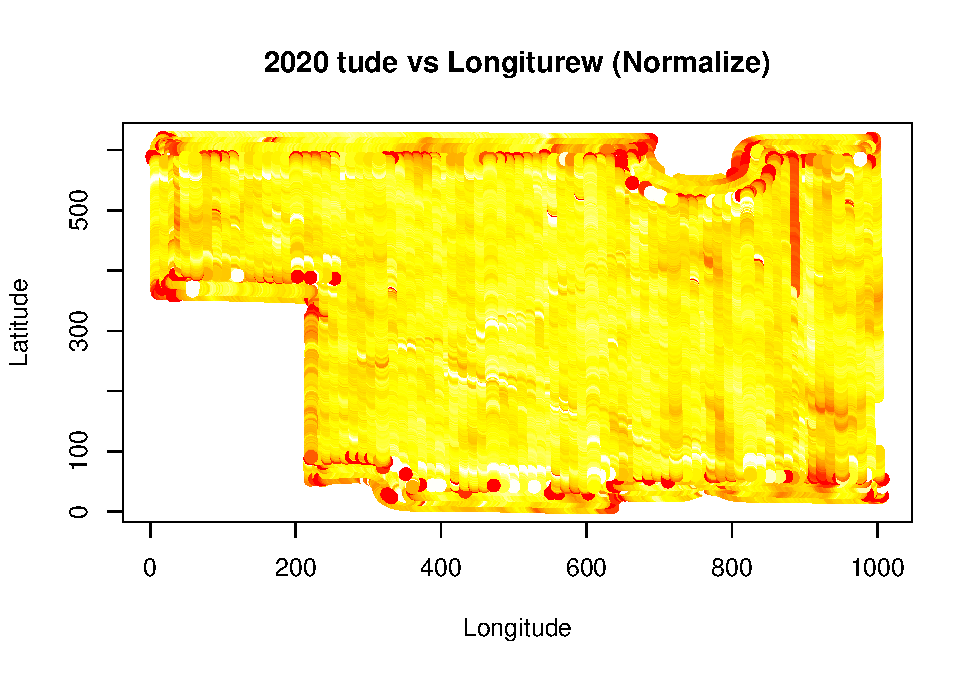
\includegraphics[keepaspectratio]{FinalProject2024X3_HR_files/figure-latex/out2020Harv-1.pdf}}

\subsubsection{2. 2020 CornHarvest Spatial Grid Format
(50mx50m)}\label{cornharvest-spatial-grid-format-50mx50m}

\begin{Shaded}
\begin{Highlighting}[]
\CommentTok{\# Subset 2020 harvest data (adjust \textquotesingle{}Type\textquotesingle{} as needed)}
\NormalTok{harvest\_2020 }\OtherTok{\textless{}{-}}\NormalTok{ Combined\_data[Combined\_data}\SpecialCharTok{$}\NormalTok{Year }\SpecialCharTok{==} \DecValTok{2020} \SpecialCharTok{\&}\NormalTok{ Combined\_data}\SpecialCharTok{$}\NormalTok{Type }\SpecialCharTok{==} \StringTok{"CornHarvest"}\NormalTok{, ]}

\CommentTok{\# Create Row and Column variables based on 50m grid using ceiling(Latitude/50) and ceiling(Longitude/50)}
\NormalTok{harvest\_2020}\SpecialCharTok{$}\NormalTok{Row }\OtherTok{\textless{}{-}} \FunctionTok{ceiling}\NormalTok{(harvest\_2020}\SpecialCharTok{$}\NormalTok{Latitude }\SpecialCharTok{/} \DecValTok{50}\NormalTok{)}
\NormalTok{harvest\_2020}\SpecialCharTok{$}\NormalTok{Column }\OtherTok{\textless{}{-}} \FunctionTok{ceiling}\NormalTok{(harvest\_2020}\SpecialCharTok{$}\NormalTok{Longitude }\SpecialCharTok{/} \DecValTok{50}\NormalTok{)}

\CommentTok{\# Create Cell identifier (Row * 1000 + Column)}
\NormalTok{harvest\_2020}\SpecialCharTok{$}\NormalTok{Cell }\OtherTok{\textless{}{-}}\NormalTok{ harvest\_2020}\SpecialCharTok{$}\NormalTok{Row }\SpecialCharTok{*} \DecValTok{1000} \SpecialCharTok{+}\NormalTok{ harvest\_2020}\SpecialCharTok{$}\NormalTok{Column}

\CommentTok{\# Aggregate mean per cell}
\NormalTok{agg\_mean }\OtherTok{\textless{}{-}} \FunctionTok{aggregate}\NormalTok{(Value }\SpecialCharTok{\textasciitilde{}}\NormalTok{ Row }\SpecialCharTok{+}\NormalTok{ Column }\SpecialCharTok{+}\NormalTok{ Cell, }\AttributeTok{data =}\NormalTok{ harvest\_2020, }\AttributeTok{FUN =}\NormalTok{ mean, }\AttributeTok{na.rm =} \ConstantTok{TRUE}\NormalTok{)}

\CommentTok{\# Aggregate count per cell}
\NormalTok{agg\_count }\OtherTok{\textless{}{-}} \FunctionTok{aggregate}\NormalTok{(Value }\SpecialCharTok{\textasciitilde{}}\NormalTok{ Row }\SpecialCharTok{+}\NormalTok{ Column }\SpecialCharTok{+}\NormalTok{ Cell, }\AttributeTok{data =}\NormalTok{ harvest\_2020, }\AttributeTok{FUN =}\NormalTok{ length)}

\CommentTok{\# Rename columns for clarity}
\FunctionTok{names}\NormalTok{(agg\_mean)[}\FunctionTok{names}\NormalTok{(agg\_mean) }\SpecialCharTok{==} \StringTok{"Value"}\NormalTok{] }\OtherTok{\textless{}{-}} \StringTok{"Mean"}
\FunctionTok{names}\NormalTok{(agg\_count)[}\FunctionTok{names}\NormalTok{(agg\_count) }\SpecialCharTok{==} \StringTok{"Value"}\NormalTok{] }\OtherTok{\textless{}{-}} \StringTok{"Count"}

\CommentTok{\# Merge mean and count}
\NormalTok{agg\_data }\OtherTok{\textless{}{-}} \FunctionTok{merge}\NormalTok{(agg\_mean, agg\_count, }\AttributeTok{by =} \FunctionTok{c}\NormalTok{(}\StringTok{"Row"}\NormalTok{, }\StringTok{"Column"}\NormalTok{, }\StringTok{"Cell"}\NormalTok{))}

\CommentTok{\# Plot Latitude \textasciitilde{} Longitude with grid lines every 50 units}
\FunctionTok{plot}\NormalTok{(harvest\_2020}\SpecialCharTok{$}\NormalTok{Longitude, harvest\_2020}\SpecialCharTok{$}\NormalTok{Latitude, }\AttributeTok{pch =} \StringTok{"."}\NormalTok{, }\AttributeTok{xlab =} \StringTok{"Longitude"}\NormalTok{, }\AttributeTok{ylab =} \StringTok{"Latitude"}\NormalTok{, }\AttributeTok{main =} \StringTok{"2020 Corn Harvest {-} 50mx50m Grid {-} Normalized"}\NormalTok{)}
\FunctionTok{abline}\NormalTok{(}\AttributeTok{h =}\NormalTok{ (}\DecValTok{1}\SpecialCharTok{:}\DecValTok{12}\NormalTok{)}\SpecialCharTok{*}\DecValTok{50}\NormalTok{, }\AttributeTok{v =}\NormalTok{ (}\DecValTok{1}\SpecialCharTok{:}\DecValTok{20}\NormalTok{)}\SpecialCharTok{*}\DecValTok{50}\NormalTok{, }\AttributeTok{col =} \StringTok{"red"}\NormalTok{, }\AttributeTok{lwd =} \DecValTok{2}\NormalTok{)}
\end{Highlighting}
\end{Shaded}

\pandocbounded{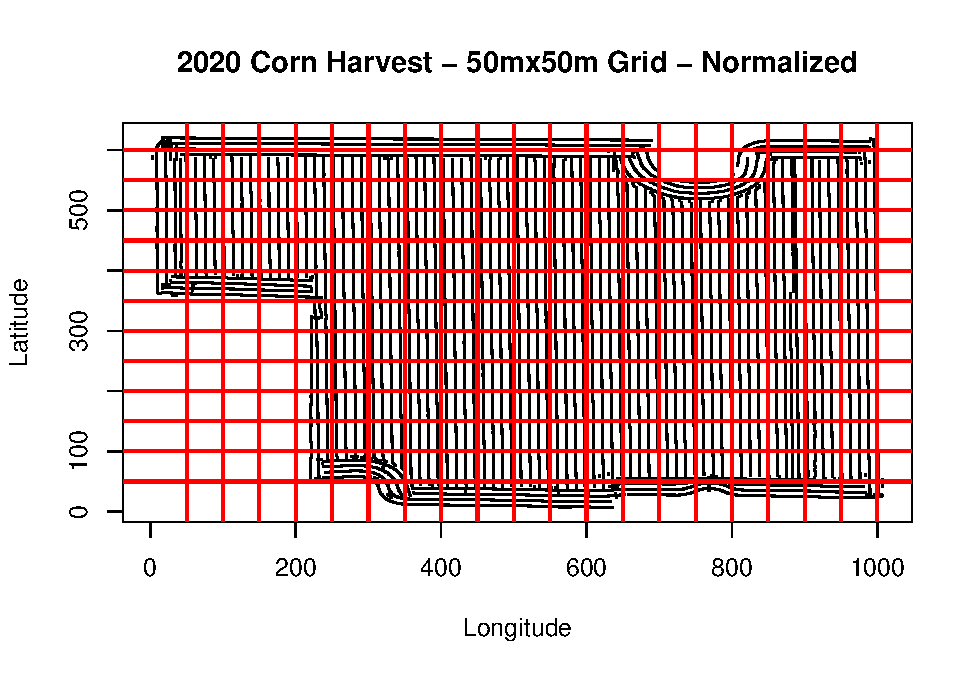
\includegraphics[keepaspectratio]{FinalProject2024X3_HR_files/figure-latex/out2020HarvGrid-1.pdf}}

\subsubsection{3. Heatmap of 2020 Corn
Yield}\label{heatmap-of-2020-corn-yield}

\begin{Shaded}
\begin{Highlighting}[]
\CommentTok{\# Corrected plotting code}
\NormalTok{plot\_data\_z }\OtherTok{\textless{}{-}}\NormalTok{ Combined\_data[}\SpecialCharTok{!}\FunctionTok{is.na}\NormalTok{(Combined\_data}\SpecialCharTok{$}\NormalTok{z\_5\_95), ]}

\NormalTok{z\_vals }\OtherTok{\textless{}{-}} \FunctionTok{as.numeric}\NormalTok{(plot\_data\_z}\SpecialCharTok{$}\NormalTok{z\_5\_95)}

\NormalTok{num\_colors }\OtherTok{\textless{}{-}} \DecValTok{100}
\NormalTok{color\_bins\_z }\OtherTok{\textless{}{-}} \FunctionTok{cut}\NormalTok{(z\_vals, }\AttributeTok{breaks =}\NormalTok{ num\_colors)}
\NormalTok{colors\_z }\OtherTok{\textless{}{-}} \FunctionTok{heat.colors}\NormalTok{(num\_colors)[}\FunctionTok{as.numeric}\NormalTok{(color\_bins\_z)]}

\FunctionTok{plot}\NormalTok{(plot\_data\_z}\SpecialCharTok{$}\NormalTok{Column, plot\_data\_z}\SpecialCharTok{$}\NormalTok{Row,}
     \AttributeTok{col =}\NormalTok{ colors\_z, }\AttributeTok{pch =} \DecValTok{15}\NormalTok{, }\AttributeTok{cex =} \FloatTok{1.5}\NormalTok{,}
     \AttributeTok{xlab =} \StringTok{"Grid Column"}\NormalTok{, }\AttributeTok{ylab =} \StringTok{"Grid Row"}\NormalTok{,}
     \AttributeTok{main =} \StringTok{"Heatmap of y20(2020 Con Yield) {-}Normalized"}\NormalTok{)}
\end{Highlighting}
\end{Shaded}

\pandocbounded{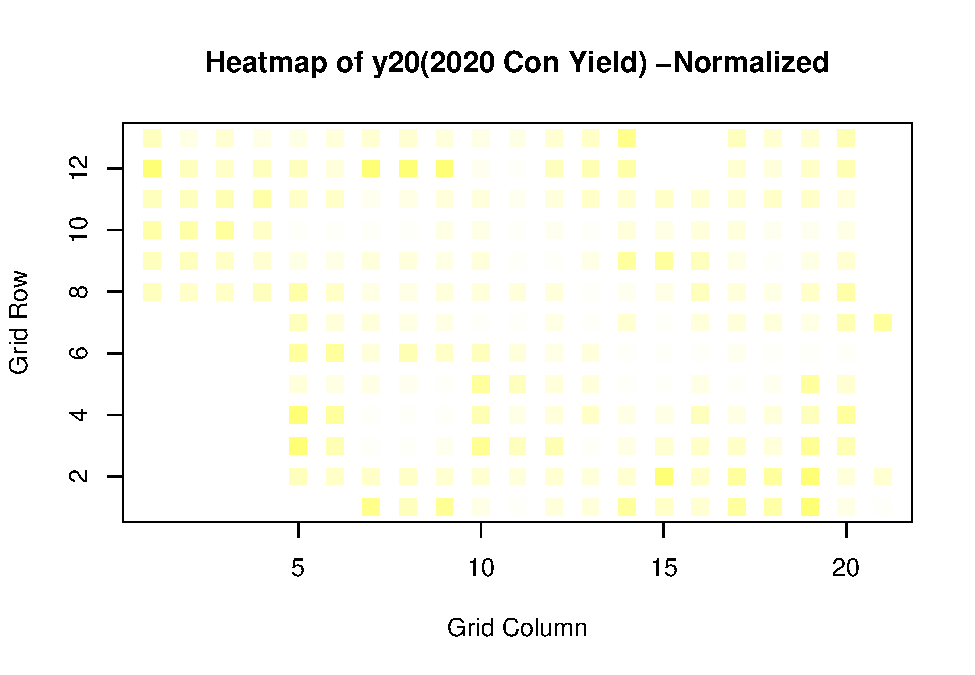
\includegraphics[keepaspectratio]{FinalProject2024X3_HR_files/figure-latex/unnamed-chunk-12-1.pdf}}

\subsubsection{4. Pairwise Relations: Yield \& Seeding Rates
(2017-2020)}\label{pairwise-relations-yield-seeding-rates-2017-2020}

\begin{Shaded}
\begin{Highlighting}[]
\CommentTok{\# Create VarYear with labels like Y17, AR18, H20, S19}
\NormalTok{Combined\_data}\SpecialCharTok{$}\NormalTok{VarYear }\OtherTok{\textless{}{-}} \FunctionTok{with}\NormalTok{(Combined\_data, \{}
\NormalTok{  abbrev }\OtherTok{\textless{}{-}} \FunctionTok{ifelse}\NormalTok{(Variable }\SpecialCharTok{==} \StringTok{"Yield"}\NormalTok{, }\StringTok{"Y"}\NormalTok{, }
                   \FunctionTok{ifelse}\NormalTok{(Variable }\SpecialCharTok{==} \StringTok{"AppliedRate"}\NormalTok{, }\StringTok{"AR"}\NormalTok{, }
                   \FunctionTok{ifelse}\NormalTok{(Type }\SpecialCharTok{==} \StringTok{"Harvest"}\NormalTok{, }\StringTok{"H"}\NormalTok{, }
                   \FunctionTok{ifelse}\NormalTok{(Type }\SpecialCharTok{==} \StringTok{"Seeding"}\NormalTok{, }\StringTok{"S"}\NormalTok{, }\ConstantTok{NA}\NormalTok{))))}
\NormalTok{  year\_short }\OtherTok{\textless{}{-}} \FunctionTok{substr}\NormalTok{(Year, }\DecValTok{3}\NormalTok{, }\DecValTok{4}\NormalTok{)}
  \FunctionTok{paste0}\NormalTok{(abbrev, year\_short)}
\NormalTok{\})}

\CommentTok{\# Aggregate: compute mean z\_5\_95 value per Cell and VarYear}
\NormalTok{agg\_data }\OtherTok{\textless{}{-}} \FunctionTok{aggregate}\NormalTok{(z\_5\_95 }\SpecialCharTok{\textasciitilde{}}\NormalTok{ Row }\SpecialCharTok{+}\NormalTok{ Column }\SpecialCharTok{+}\NormalTok{ VarYear, }
                      \AttributeTok{data =}\NormalTok{ Combined\_data, }\AttributeTok{FUN =}\NormalTok{ mean)}

\CommentTok{\# Reshape from long to wide}
\NormalTok{wide\_data }\OtherTok{\textless{}{-}} \FunctionTok{reshape}\NormalTok{(}\AttributeTok{data =}\NormalTok{ agg\_data,}
                     \AttributeTok{idvar =} \FunctionTok{c}\NormalTok{(}\StringTok{"Row"}\NormalTok{, }\StringTok{"Column"}\NormalTok{),}
                     \AttributeTok{timevar =} \StringTok{"VarYear"}\NormalTok{,}
                     \AttributeTok{direction =} \StringTok{"wide"}\NormalTok{)}

\CommentTok{\# Clean column names}
\FunctionTok{names}\NormalTok{(wide\_data) }\OtherTok{\textless{}{-}} \FunctionTok{sub}\NormalTok{(}\StringTok{"z\_5\_95}\SpecialCharTok{\textbackslash{}\textbackslash{}}\StringTok{."}\NormalTok{, }\StringTok{""}\NormalTok{, }\FunctionTok{names}\NormalTok{(wide\_data))}

\CommentTok{\# Remove rows with NAs}
\NormalTok{clean\_data }\OtherTok{\textless{}{-}} \FunctionTok{na.omit}\NormalTok{(wide\_data)}

\CommentTok{\# Create pairs plot}
\FunctionTok{pairs}\NormalTok{(clean\_data[, }\SpecialCharTok{{-}}\FunctionTok{c}\NormalTok{(}\DecValTok{1}\NormalTok{, }\DecValTok{2}\NormalTok{)],}
      \AttributeTok{main =} \StringTok{"Pairs Plot: Normalized Aggregated Data"}\NormalTok{)}
\end{Highlighting}
\end{Shaded}

\pandocbounded{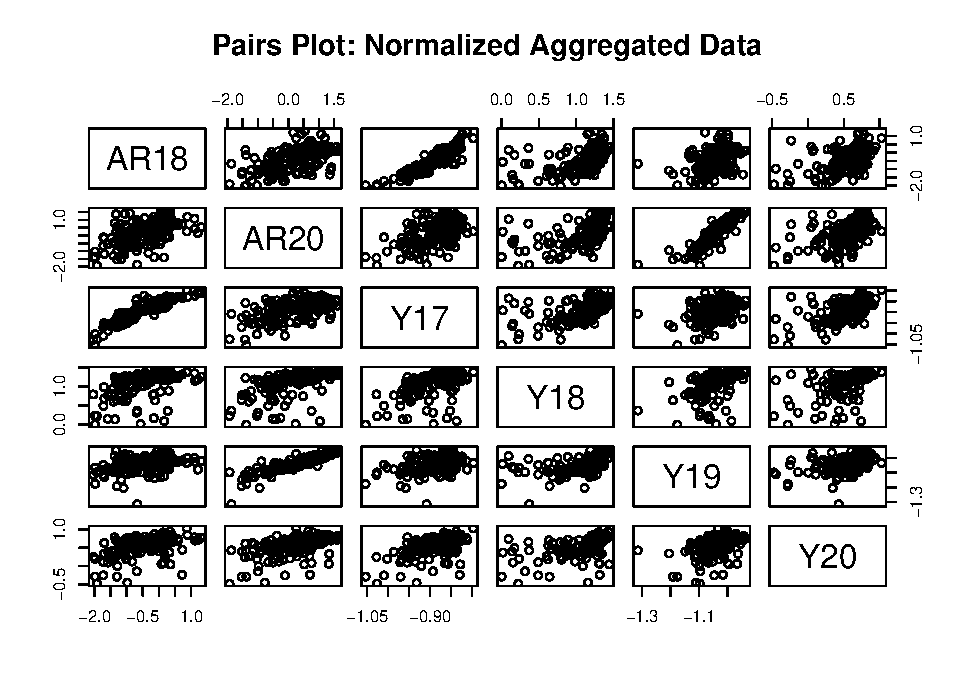
\includegraphics[keepaspectratio]{FinalProject2024X3_HR_files/figure-latex/pairPltNorm-1.pdf}}

\subsubsection{5. Visualized Combined Normalized Data
View}\label{visualized-combined-normalized-data-view}

\begin{Shaded}
\begin{Highlighting}[]
\NormalTok{create\_wide\_summary }\OtherTok{\textless{}{-}} \ControlFlowTok{function}\NormalTok{(data, value\_col, }\AttributeTok{summary\_fun =}\NormalTok{ mean, ...) \{}
  \CommentTok{\# Ensure the value column exists}
  \ControlFlowTok{if}\NormalTok{ (}\SpecialCharTok{!}\NormalTok{value\_col }\SpecialCharTok{\%in\%} \FunctionTok{names}\NormalTok{(data)) \{}
    \FunctionTok{stop}\NormalTok{(}\FunctionTok{paste}\NormalTok{(}\StringTok{"Column"}\NormalTok{, value\_col, }\StringTok{"not found in data."}\NormalTok{))}
\NormalTok{  \}}

  \CommentTok{\# Dynamically create the formula: value\_col \textasciitilde{} Row + Column + VarYear}
\NormalTok{  formula\_str }\OtherTok{\textless{}{-}} \FunctionTok{paste}\NormalTok{(value\_col, }\StringTok{"\textasciitilde{} Row + Column + VarYear"}\NormalTok{)}
\NormalTok{  formula\_obj }\OtherTok{\textless{}{-}} \FunctionTok{as.formula}\NormalTok{(formula\_str)}

  \CommentTok{\# Aggregate the data}
\NormalTok{  agg\_data }\OtherTok{\textless{}{-}} \FunctionTok{aggregate}\NormalTok{(formula\_obj,}
                        \AttributeTok{data =}\NormalTok{ data,}
                        \AttributeTok{FUN =}\NormalTok{ summary\_fun,}
\NormalTok{                        ...)}

  \CommentTok{\# Reshape to wide format}
\NormalTok{  wide\_data }\OtherTok{\textless{}{-}} \FunctionTok{reshape}\NormalTok{(agg\_data,}
                       \AttributeTok{idvar =} \FunctionTok{c}\NormalTok{(}\StringTok{"Row"}\NormalTok{, }\StringTok{"Column"}\NormalTok{),}
                       \AttributeTok{timevar =} \StringTok{"VarYear"}\NormalTok{,}
                       \AttributeTok{direction =} \StringTok{"wide"}\NormalTok{)}
  
  \CommentTok{\# Sort value columns by year suffix}
\NormalTok{  id\_cols }\OtherTok{\textless{}{-}} \FunctionTok{c}\NormalTok{(}\StringTok{"Row"}\NormalTok{, }\StringTok{"Column"}\NormalTok{)}
\NormalTok{  value\_cols }\OtherTok{\textless{}{-}} \FunctionTok{setdiff}\NormalTok{(}\FunctionTok{names}\NormalTok{(wide\_data), id\_cols)}

  \CommentTok{\# Extract year suffix (17, 18,...) from column names and sort}
\NormalTok{  sorted\_value\_cols }\OtherTok{\textless{}{-}}\NormalTok{ value\_cols[}\FunctionTok{order}\NormalTok{(}\FunctionTok{as.numeric}\NormalTok{(}\FunctionTok{sub}\NormalTok{(}\StringTok{".*}\SpecialCharTok{\textbackslash{}\textbackslash{}}\StringTok{."}\NormalTok{, }\StringTok{""}\NormalTok{, value\_cols)))]}

  \CommentTok{\# Create numeric Cell ID}
\NormalTok{  wide\_data}\SpecialCharTok{$}\NormalTok{Cell }\OtherTok{\textless{}{-}}\NormalTok{ wide\_data}\SpecialCharTok{$}\NormalTok{Row }\SpecialCharTok{*} \DecValTok{1000} \SpecialCharTok{+}\NormalTok{ wide\_data}\SpecialCharTok{$}\NormalTok{Column}

  \CommentTok{\# Reorder: place Cell followed by sorted values }
\NormalTok{  wide\_data }\OtherTok{\textless{}{-}}\NormalTok{ wide\_data[, }\FunctionTok{c}\NormalTok{(}\StringTok{"Cell"}\NormalTok{, sorted\_value\_cols)]}

  \FunctionTok{return}\NormalTok{(wide\_data)}
\NormalTok{\}}
\end{Highlighting}
\end{Shaded}

Notes: Sorted values in order:
\((\text{AR17}, \text{AR18}, \text{Y17}, \text{etc.})\)

\subsubsection{Visualized Merge Normalized
Dataset}\label{visualized-merge-normalized-dataset}

\begin{Shaded}
\begin{Highlighting}[]
\NormalTok{wide\_z5\_95 }\OtherTok{\textless{}{-}} \FunctionTok{create\_wide\_summary}\NormalTok{(Combined\_data, }\StringTok{"z\_5\_95"}\NormalTok{, mean, }\AttributeTok{na.rm =} \ConstantTok{TRUE}\NormalTok{)}
\end{Highlighting}
\end{Shaded}

\begin{verbatim}
## Warning in eval(quote(list(...)), env): NAs introduced by coercion
\end{verbatim}

\begin{Shaded}
\begin{Highlighting}[]
\FunctionTok{head}\NormalTok{(wide\_z5\_95)}
\end{Highlighting}
\end{Shaded}

\begin{verbatim}
##    Cell z_5_95.AR18 z_5_95.AR20 z_5_95.Y17 z_5_95.Y18 z_5_95.Y19 z_5_95.Y20
## 1  8001  -1.9213284  -1.9358509 -1.0265580  0.2246157  -1.097718 -0.4744617
## 2  9001  -0.7706741  -0.4971648 -0.9330765  0.8997355  -1.085984  0.5122085
## 3 10001  -1.2134839  -0.4323335 -0.9234435  0.9534400  -1.061734  0.4014553
## 4 11001  -0.8111415  -0.7616415 -0.9247440  0.8415962  -1.102783  0.6354213
## 5 12001  -0.9813489  -0.4879879 -0.9503524  0.6643643  -1.075339  0.4658139
## 6  8002  -1.3596746  -0.4174676 -0.9653397  0.1416735  -1.060955  0.3992695
\end{verbatim}

\#\#\#6. Causual Analysis - DAG for SCALED DATASET Since DAGs only show
data dependencies, note is made that DAGs using normalized data would
reveal similar strengths as those for the raw data presented earlier.
will only produce a full model DAG (2017-2020) here, using our
normalized dataset.

\subsubsection{i. DAG model for 2017 -
2020}\label{i.-dag-model-for-2017---2020}

\begin{Shaded}
\begin{Highlighting}[]
\FunctionTok{library}\NormalTok{(bnlearn)}
\FunctionTok{library}\NormalTok{(Rgraphviz)}

\CommentTok{\# Rename columns in wide\_z5\_95 just once}
\FunctionTok{colnames}\NormalTok{(wide\_z5\_95) }\OtherTok{\textless{}{-}} \FunctionTok{sub}\NormalTok{(}\StringTok{"\^{}z\_5\_95}\SpecialCharTok{\textbackslash{}\textbackslash{}}\StringTok{."}\NormalTok{, }\StringTok{"z."}\NormalTok{, }\FunctionTok{colnames}\NormalTok{(wide\_z5\_95))}

\CommentTok{\# Prepare modeling data}
\NormalTok{model\_data\_z }\OtherTok{\textless{}{-}}\NormalTok{ wide\_z5\_95[, }\FunctionTok{c}\NormalTok{(}\StringTok{"z.Y17"}\NormalTok{, }\StringTok{"z.AR18"}\NormalTok{, }\StringTok{"z.Y18"}\NormalTok{, }\StringTok{"z.Y19"}\NormalTok{, }\StringTok{"z.AR20"}\NormalTok{, }\StringTok{"z.Y20"}\NormalTok{)]}
\NormalTok{model\_data\_z }\OtherTok{\textless{}{-}} \FunctionTok{na.omit}\NormalTok{(model\_data\_z)}

\CommentTok{\#"Cell"   "z.AR18" "z.AR20" "z.Y17"  "z.Y18"  "z.Y19"  "z.Y20" }

\CommentTok{\# Regression Model created}
\CommentTok{\#model\_Y20\_z \textless{}{-} lm(z.Y20 \textasciitilde{} z.Y17 + z.Y18 + z.Y19 + z.AR18 + z.AR20, data = \#model\_data\_z)}
\CommentTok{\#summary(model\_Y20\_z)}

\NormalTok{modela.dag }\OtherTok{\textless{}{-}} \FunctionTok{model2network}\NormalTok{(}\StringTok{"[z.Y17][z.AR18|z.Y17][z.Y18|z.AR18:z.Y17]"}\NormalTok{)}

\CommentTok{\# Subset to match DAG variables}
\NormalTok{data\_a }\OtherTok{\textless{}{-}}\NormalTok{ model\_data\_z[, }\FunctionTok{c}\NormalTok{(}\StringTok{"z.Y17"}\NormalTok{, }\StringTok{"z.AR18"}\NormalTok{, }\StringTok{"z.Y18"}\NormalTok{)]}
\CommentTok{\# Fit and plot}
\NormalTok{fita }\OtherTok{\textless{}{-}} \FunctionTok{bn.fit}\NormalTok{(modela.dag, data\_a)}
\NormalTok{strengtha }\OtherTok{\textless{}{-}} \FunctionTok{arc.strength}\NormalTok{(modela.dag, data\_a)}
\CommentTok{\#strength.plot(modela.dag, strengtha)}

\CommentTok{\# Define DAG}
\NormalTok{modelb.dag }\OtherTok{\textless{}{-}} \FunctionTok{model2network}\NormalTok{(}\StringTok{"[z.Y19][z.AR20|z.Y19][z.Y20|z.AR20:z.Y19]"}\NormalTok{)}

\CommentTok{\# Subset data to include only the nodes in the DAG}
\NormalTok{data\_b }\OtherTok{\textless{}{-}}\NormalTok{ model\_data\_z[, }\FunctionTok{c}\NormalTok{(}\StringTok{"z.Y19"}\NormalTok{, }\StringTok{"z.AR20"}\NormalTok{, }\StringTok{"z.Y20"}\NormalTok{)]}

\CommentTok{\# Fit and plot}
\NormalTok{fitb }\OtherTok{\textless{}{-}} \FunctionTok{bn.fit}\NormalTok{(modelb.dag, data\_b)}
\NormalTok{strengthb }\OtherTok{\textless{}{-}} \FunctionTok{arc.strength}\NormalTok{(modelb.dag, data\_b)}
\CommentTok{\#strength.plot(modelb.dag, strengthb)}


\CommentTok{\# DAG c {-} representing combination}
\CommentTok{\#modelc.dag \textless{}{-} model2network("[z.Y17][z.AR18|z.Y17][z.Y18|z.AR18:z.Y17][z.Y19|z.Y17:z.AR18:z.Y18][z.AR20|z.Y19][z.Y20|z.AR20:z.Y19]")}
\NormalTok{modelc.dag }\OtherTok{\textless{}{-}} \FunctionTok{model2network}\NormalTok{(}\StringTok{"[z.Y17][z.AR18|z.Y17][z.Y18|z.AR18:z.Y17][z.Y19|z.Y17:z.AR18:z.Y18][z.AR20|z.Y19][z.Y20|z.AR20:z.Y19]"}\NormalTok{)}
\NormalTok{fitc }\OtherTok{\textless{}{-}} \FunctionTok{bn.fit}\NormalTok{(modelc.dag, model\_data\_z)}
\NormalTok{strengthc }\OtherTok{\textless{}{-}} \FunctionTok{arc.strength}\NormalTok{(modelc.dag, model\_data\_z)}
\FunctionTok{strength.plot}\NormalTok{(modelc.dag, strengthc)}
\end{Highlighting}
\end{Shaded}

\pandocbounded{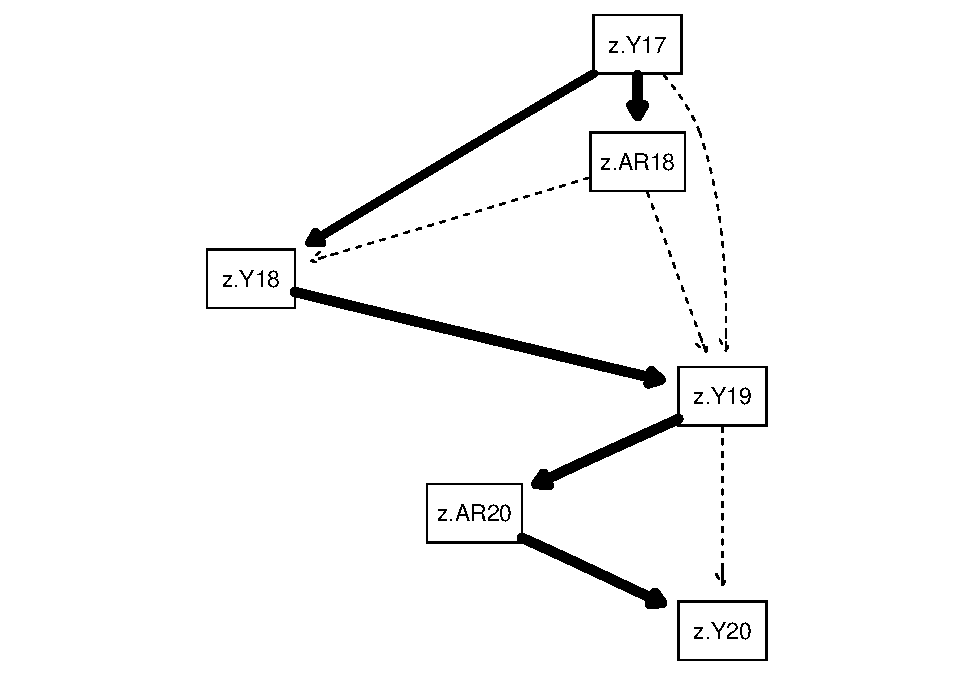
\includegraphics[keepaspectratio]{FinalProject2024X3_HR_files/figure-latex/combDtaDirGraph_17_20Norm-1.pdf}}

\begin{Shaded}
\begin{Highlighting}[]
\CommentTok{\#sort(nodes(modelc.dag))}
\end{Highlighting}
\end{Shaded}

\begin{Shaded}
\begin{Highlighting}[]
\CommentTok{\#sort(nodes(modelc.dag)) == sort(colnames(model\_data\_z))}
\end{Highlighting}
\end{Shaded}

\subsubsection{7. DAG COMPARISON - RAW (below) vs NORMALIZED
(above)}\label{dag-comparison---raw-below-vs-normalized-above}

\textbf{ANALYSIS:} We observe that the structure of the DAG of the Raw
dataset (visual at \(6.f.iii\)) and that of the normalized dataset are
similar. The same conclusion can therefore be drawn - that the yield
rate of 2017 is a good predictor for the yield rate of 2020. Hence,
\textbf{normalization preseved the structure of a DAG.}

Will proceed to test the strength of these links to fully verify our
project's objective: whether a relationship exists between the
\emph{yield and the applied seeding and/or yield (previous years)}.

\subsubsection{Calculated Strengths of DAG:
2017-2020}\label{calculated-strengths-of-dag-2017-2020}

\paragraph{7a. Arc Strengths of Raw
Data}\label{a.-arc-strengths-of-raw-data}

\begin{Shaded}
\begin{Highlighting}[]
\FunctionTok{library}\NormalTok{(bnlearn)}

\NormalTok{model\_data\_raw }\OtherTok{\textless{}{-}}\NormalTok{ Combined3[, }\FunctionTok{c}\NormalTok{(}\StringTok{"Y17"}\NormalTok{, }\StringTok{"Y18"}\NormalTok{, }\StringTok{"Y20"}\NormalTok{, }\StringTok{"AR18"}\NormalTok{)]}
\NormalTok{model\_data\_raw }\OtherTok{\textless{}{-}} \FunctionTok{na.omit}\NormalTok{(model\_data\_raw)}

\CommentTok{\# Learn the network structure}
\NormalTok{modelc.dag }\OtherTok{\textless{}{-}} \FunctionTok{hc}\NormalTok{(model\_data\_raw)  }

\CommentTok{\# Compute arc strength values using test{-}based criterion RAW}
\NormalTok{Rstrength\_df }\OtherTok{\textless{}{-}} \FunctionTok{arc.strength}\NormalTok{(modelc.dag, }\AttributeTok{data =}\NormalTok{ model\_data\_raw, }\AttributeTok{criterion =} \StringTok{"cor"}\NormalTok{)}

\CommentTok{\# View the first few rows}
\CommentTok{\# head(Rstrength\_df)}

\CommentTok{\# Sort the  strengths}
\NormalTok{Rsorted\_strengths}\OtherTok{\textless{}{-}}\NormalTok{ Rstrength\_df[}\FunctionTok{order}\NormalTok{(}\SpecialCharTok{{-}}\NormalTok{Rstrength\_df}\SpecialCharTok{$}\NormalTok{strength), ]}

\NormalTok{Rsorted\_strengths}
\end{Highlighting}
\end{Shaded}

\begin{verbatim}
##   from   to     strength
## 5 AR18  Y20 4.768041e-03
## 4  Y18  Y20 1.034353e-06
## 3  Y17  Y20 5.584207e-08
## 2  Y17  Y18 7.614679e-24
## 1  Y17 AR18 6.864785e-75
\end{verbatim}

\subsubsection{7b. Arc Strengths of Normalized
Data}\label{b.-arc-strengths-of-normalized-data}

\begin{Shaded}
\begin{Highlighting}[]
\FunctionTok{library}\NormalTok{(bnlearn)}

\CommentTok{\# Learn the network structure}
\NormalTok{modelc.dag }\OtherTok{\textless{}{-}} \FunctionTok{hc}\NormalTok{(model\_data\_z)  }

\CommentTok{\# Compute arc strength values using test{-}based criterion}
\NormalTok{Nstrength\_df }\OtherTok{\textless{}{-}} \FunctionTok{arc.strength}\NormalTok{(modelc.dag, }\AttributeTok{data =}\NormalTok{ model\_data\_z, }\AttributeTok{criterion =} \StringTok{"cor"}\NormalTok{)}

\CommentTok{\# View the first few rows}
\CommentTok{\#head(Nstrength\_df)}

\CommentTok{\# Sort the  strengths}
\NormalTok{Nsorted\_strengths }\OtherTok{\textless{}{-}}\NormalTok{ Nstrength\_df[}\FunctionTok{order}\NormalTok{(}\SpecialCharTok{{-}}\NormalTok{Nstrength\_df}\SpecialCharTok{$}\NormalTok{strength), ]}

\NormalTok{Nsorted\_strengths}
\end{Highlighting}
\end{Shaded}

\begin{verbatim}
##      from     to     strength
## 10  z.Y19 z.AR18 1.817041e-02
## 8   z.Y18  z.Y20 5.103262e-03
## 9  z.AR20 z.AR18 6.818397e-04
## 6  z.AR20  z.Y20 3.973602e-04
## 4   z.Y17  z.Y20 8.038124e-07
## 7  z.AR20  z.Y17 6.023703e-07
## 5   z.Y18  z.Y17 2.884985e-07
## 3  z.AR20  z.Y18 3.276752e-22
## 1   z.Y17 z.AR18 6.654734e-58
## 2   z.Y19 z.AR20 1.119163e-75
\end{verbatim}

\textbf{Arc Length Comparisons:}

\begin{itemize}
\item
  Varying number of reporting arc strengths for the Raw (5) and Normal
  (10) datasets.
\item
  In the Raw dataset, the strongest link is between Y18 and Y20
  \((4.768041e-08)\) while that for the Normalized dataset is between
  zY19 and zAR20 \((1.817041e-02\). We note too the difference in
  magnitude in the top level supporting links.
\item
  In the Raw dataset, the weakest link is between Y17 and AR18
  \((6.864785e-75)\) while that for the Normalized dataset is between
  zY19 and zAR18 \((1.119163e-75)\) . We note too the difference in
  magnitude in the bottom level supporting links.
\item
  Numerically, though, the Normalized dataset has the highest strength
\item
  The normalized model retains and clarifies the core structural
  relationships among key agricultural variables (e.g., yield, applied
  rate across years). The arc strengths, especially the top quartile,
  reinforce the robustness of these relationships. Overall, the
  normalization process has enhanced interpretability and reduced
  scale-driven bias, making the Bayesian network structure more stable
  for downstream inference.
\end{itemize}

\subsubsection{7c: Arc Length Density plots \& Summary
Stats}\label{c-arc-length-density-plots-summary-stats}

\begin{Shaded}
\begin{Highlighting}[]
\CommentTok{\# Load bnlearn}
\FunctionTok{library}\NormalTok{(bnlearn)}

\NormalTok{model\_data\_raw }\OtherTok{\textless{}{-}}\NormalTok{ Combined3[, }\FunctionTok{c}\NormalTok{(}\StringTok{"Y17"}\NormalTok{, }\StringTok{"Y18"}\NormalTok{, }\StringTok{"Y20"}\NormalTok{, }\StringTok{"AR18"}\NormalTok{)]}
\NormalTok{model\_data\_raw }\OtherTok{\textless{}{-}} \FunctionTok{na.omit}\NormalTok{(model\_data\_raw)}

\CommentTok{\# Compute arc strengths of both moderls}
\NormalTok{arc\_raw }\OtherTok{\textless{}{-}} \FunctionTok{arc.strength}\NormalTok{(}\FunctionTok{hc}\NormalTok{(model\_data\_raw), }\AttributeTok{data =}\NormalTok{ model\_data\_raw, }\AttributeTok{criterion =} \StringTok{"cor"}\NormalTok{)}
\NormalTok{arc\_norm }\OtherTok{\textless{}{-}} \FunctionTok{arc.strength}\NormalTok{(}\FunctionTok{hc}\NormalTok{(model\_data\_z), }\AttributeTok{data =}\NormalTok{ model\_data\_z, }\AttributeTok{criterion =} \StringTok{"cor"}\NormalTok{)}

\CommentTok{\# Add source column manually}
\NormalTok{arc\_raw}\SpecialCharTok{$}\NormalTok{Source }\OtherTok{\textless{}{-}} \StringTok{"Raw"}
\NormalTok{arc\_norm}\SpecialCharTok{$}\NormalTok{Source }\OtherTok{\textless{}{-}} \StringTok{"Normalized"}

\CommentTok{\# Combine both datasets}
\NormalTok{arc\_combined }\OtherTok{\textless{}{-}} \FunctionTok{rbind}\NormalTok{(arc\_raw, arc\_norm)}

\CommentTok{\# Set up the plot layout}
\FunctionTok{par}\NormalTok{(}\AttributeTok{mfrow =} \FunctionTok{c}\NormalTok{(}\DecValTok{1}\NormalTok{, }\DecValTok{1}\NormalTok{))  }\CommentTok{\# 1 panel}

\CommentTok{\# Density plots}
\FunctionTok{plot}\NormalTok{(}\FunctionTok{density}\NormalTok{(arc\_raw}\SpecialCharTok{$}\NormalTok{strength),}
     \AttributeTok{col =} \StringTok{"blue"}\NormalTok{, }\AttributeTok{lwd =} \DecValTok{2}\NormalTok{, }\AttributeTok{main =} \StringTok{"Arc Strength Distribution"}\NormalTok{,}
     \AttributeTok{xlab =} \StringTok{"Arc Strength"}\NormalTok{, }\AttributeTok{ylim =} \FunctionTok{c}\NormalTok{(}\DecValTok{0}\NormalTok{, }\FunctionTok{max}\NormalTok{(}\FunctionTok{density}\NormalTok{(arc\_raw}\SpecialCharTok{$}\NormalTok{strength)}\SpecialCharTok{$}\NormalTok{y, }\FunctionTok{density}\NormalTok{(arc\_norm}\SpecialCharTok{$}\NormalTok{strength)}\SpecialCharTok{$}\NormalTok{y)))}
\FunctionTok{lines}\NormalTok{(}\FunctionTok{density}\NormalTok{(arc\_norm}\SpecialCharTok{$}\NormalTok{strength), }\AttributeTok{col =} \StringTok{"red"}\NormalTok{, }\AttributeTok{lwd =} \DecValTok{2}\NormalTok{, }\AttributeTok{lty =} \DecValTok{2}\NormalTok{)}
\FunctionTok{legend}\NormalTok{(}\StringTok{"topright"}\NormalTok{, }\AttributeTok{legend =} \FunctionTok{c}\NormalTok{(}\StringTok{"Raw"}\NormalTok{, }\StringTok{"Normalized"}\NormalTok{), }\AttributeTok{col =} \FunctionTok{c}\NormalTok{(}\StringTok{"blue"}\NormalTok{, }\StringTok{"red"}\NormalTok{), }\AttributeTok{lwd =} \DecValTok{2}\NormalTok{, }\AttributeTok{lty =} \FunctionTok{c}\NormalTok{(}\DecValTok{1}\NormalTok{, }\DecValTok{2}\NormalTok{))}
\end{Highlighting}
\end{Shaded}

\pandocbounded{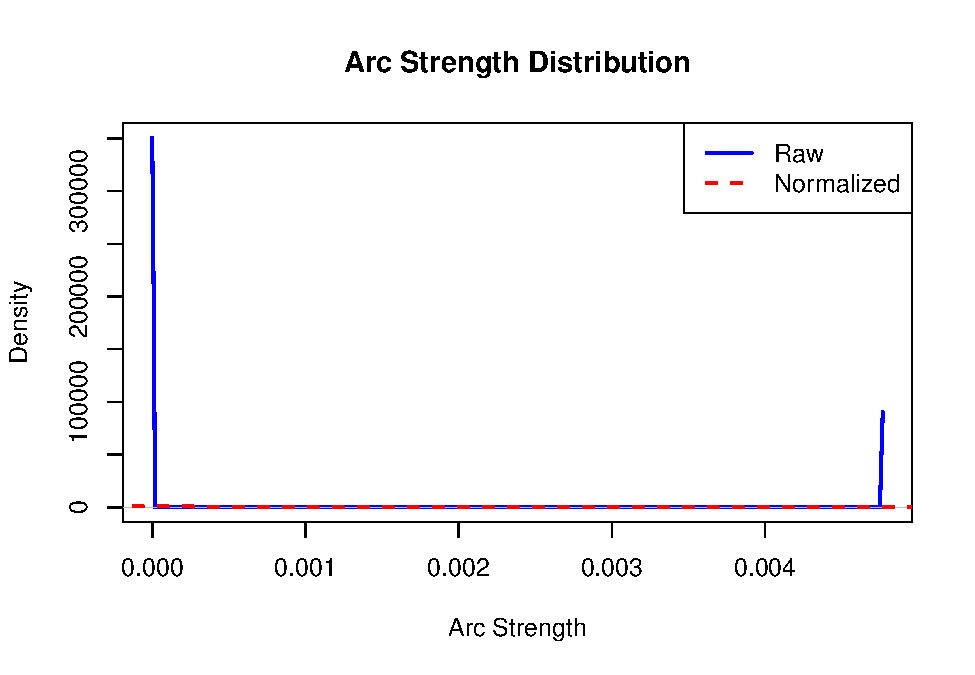
\includegraphics[keepaspectratio]{FinalProject2024X3_HR_files/figure-latex/compArcStrength-1.pdf}}

\begin{Shaded}
\begin{Highlighting}[]
\CommentTok{\# Descriptive statistics for each datasets}
\NormalTok{summary\_raw }\OtherTok{\textless{}{-}} \FunctionTok{c}\NormalTok{(}
  \AttributeTok{Mean =} \FunctionTok{mean}\NormalTok{(arc\_raw}\SpecialCharTok{$}\NormalTok{strength),}
  \AttributeTok{Median =} \FunctionTok{median}\NormalTok{(arc\_raw}\SpecialCharTok{$}\NormalTok{strength),}
  \AttributeTok{SD =} \FunctionTok{sd}\NormalTok{(arc\_raw}\SpecialCharTok{$}\NormalTok{strength),}
  \AttributeTok{Min =} \FunctionTok{min}\NormalTok{(arc\_raw}\SpecialCharTok{$}\NormalTok{strength),}
  \AttributeTok{Max =} \FunctionTok{max}\NormalTok{(arc\_raw}\SpecialCharTok{$}\NormalTok{strength),}
  \AttributeTok{Count =} \FunctionTok{length}\NormalTok{(arc\_raw}\SpecialCharTok{$}\NormalTok{strength)}
\NormalTok{)}

\NormalTok{summary\_norm }\OtherTok{\textless{}{-}} \FunctionTok{c}\NormalTok{(}
  \AttributeTok{Mean =} \FunctionTok{mean}\NormalTok{(arc\_norm}\SpecialCharTok{$}\NormalTok{strength),}
  \AttributeTok{Median =} \FunctionTok{median}\NormalTok{(arc\_norm}\SpecialCharTok{$}\NormalTok{strength),}
  \AttributeTok{SD =} \FunctionTok{sd}\NormalTok{(arc\_norm}\SpecialCharTok{$}\NormalTok{strength),}
  \AttributeTok{Min =} \FunctionTok{min}\NormalTok{(arc\_norm}\SpecialCharTok{$}\NormalTok{strength),}
  \AttributeTok{Max =} \FunctionTok{max}\NormalTok{(arc\_norm}\SpecialCharTok{$}\NormalTok{strength),}
  \AttributeTok{Count =} \FunctionTok{length}\NormalTok{(arc\_norm}\SpecialCharTok{$}\NormalTok{strength)}
\NormalTok{)}

\CommentTok{\# Print summary stats side by side}
\NormalTok{comparison\_table }\OtherTok{\textless{}{-}} \FunctionTok{rbind}\NormalTok{(}\AttributeTok{Raw =}\NormalTok{ summary\_raw, }\AttributeTok{Normalized =}\NormalTok{ summary\_norm)}
\FunctionTok{print}\NormalTok{(}\FunctionTok{round}\NormalTok{(comparison\_table, }\DecValTok{4}\NormalTok{))}
\end{Highlighting}
\end{Shaded}

\begin{verbatim}
##              Mean Median     SD Min    Max Count
## Raw        0.0010      0 0.0021   0 0.0048     5
## Normalized 0.0024      0 0.0057   0 0.0182    10
\end{verbatim}

\begin{Shaded}
\begin{Highlighting}[]
\CommentTok{\# Fix the column names of the normalized dataset to match raw}
\FunctionTok{colnames}\NormalTok{(model\_data\_z) }\OtherTok{\textless{}{-}} \FunctionTok{gsub}\NormalTok{(}\StringTok{"\^{}z}\SpecialCharTok{\textbackslash{}\textbackslash{}}\StringTok{."}\NormalTok{, }\StringTok{""}\NormalTok{, }\FunctionTok{colnames}\NormalTok{(model\_data\_z))}

\CommentTok{\# Learn network structures}
\NormalTok{fit\_raw }\OtherTok{\textless{}{-}} \FunctionTok{hc}\NormalTok{(model\_data\_raw)}
\NormalTok{fit\_norm }\OtherTok{\textless{}{-}} \FunctionTok{hc}\NormalTok{(model\_data\_z)}

\CommentTok{\# Compute arc strengths}
\NormalTok{raw\_strength }\OtherTok{\textless{}{-}} \FunctionTok{arc.strength}\NormalTok{(fit\_raw, }\AttributeTok{data =}\NormalTok{ model\_data\_raw)}
\NormalTok{norm\_strength }\OtherTok{\textless{}{-}} \FunctionTok{arc.strength}\NormalTok{(fit\_norm, }\AttributeTok{data =}\NormalTok{ model\_data\_z)}

\CommentTok{\# Create arc\_id with sorted node names}
\NormalTok{raw\_strength}\SpecialCharTok{$}\NormalTok{arc\_id }\OtherTok{\textless{}{-}} \FunctionTok{apply}\NormalTok{(raw\_strength[, }\FunctionTok{c}\NormalTok{(}\StringTok{"from"}\NormalTok{, }\StringTok{"to"}\NormalTok{)], }\DecValTok{1}\NormalTok{, }\ControlFlowTok{function}\NormalTok{(x) }\FunctionTok{paste}\NormalTok{(}\FunctionTok{sort}\NormalTok{(x), }\AttributeTok{collapse =} \StringTok{"\_"}\NormalTok{))}
\NormalTok{norm\_strength}\SpecialCharTok{$}\NormalTok{arc\_id }\OtherTok{\textless{}{-}} \FunctionTok{apply}\NormalTok{(norm\_strength[, }\FunctionTok{c}\NormalTok{(}\StringTok{"from"}\NormalTok{, }\StringTok{"to"}\NormalTok{)], }\DecValTok{1}\NormalTok{, }\ControlFlowTok{function}\NormalTok{(x) }\FunctionTok{paste}\NormalTok{(}\FunctionTok{sort}\NormalTok{(x), }\AttributeTok{collapse =} \StringTok{"\_"}\NormalTok{))}

\CommentTok{\# Merge arc strengths by arc\_id}
\NormalTok{merged\_arcs }\OtherTok{\textless{}{-}} \FunctionTok{merge}\NormalTok{(}
\NormalTok{  raw\_strength[, }\FunctionTok{c}\NormalTok{(}\StringTok{"arc\_id"}\NormalTok{, }\StringTok{"strength"}\NormalTok{)],}
\NormalTok{  norm\_strength[, }\FunctionTok{c}\NormalTok{(}\StringTok{"arc\_id"}\NormalTok{, }\StringTok{"strength"}\NormalTok{)],}
  \AttributeTok{by =} \StringTok{"arc\_id"}\NormalTok{,}
  \AttributeTok{suffixes =} \FunctionTok{c}\NormalTok{(}\StringTok{"\_raw"}\NormalTok{, }\StringTok{"\_norm"}\NormalTok{)}
\NormalTok{)}

\CommentTok{\# Reconstruct readable arc labels}
\NormalTok{merged\_arcs}\SpecialCharTok{$}\NormalTok{arc }\OtherTok{\textless{}{-}} \FunctionTok{gsub}\NormalTok{(}\StringTok{"\_"}\NormalTok{, }\StringTok{" ↔ "}\NormalTok{, merged\_arcs}\SpecialCharTok{$}\NormalTok{arc\_id)}

\CommentTok{\# Sort by raw strength}
\NormalTok{merged\_arcs }\OtherTok{\textless{}{-}}\NormalTok{ merged\_arcs[}\FunctionTok{order}\NormalTok{(}\SpecialCharTok{{-}}\NormalTok{merged\_arcs}\SpecialCharTok{$}\NormalTok{strength\_raw), ]}

\CommentTok{\# View result}
\FunctionTok{print}\NormalTok{(merged\_arcs)}
\end{Highlighting}
\end{Shaded}

\begin{verbatim}
##     arc_id strength_raw strength_norm        arc
## 4  Y18_Y20    -9.540109     -1.347586  Y18 ↔ Y20
## 3  Y17_Y20   -12.423925     -9.788422  Y17 ↔ Y20
## 2  Y17_Y18   -48.658839    -10.733874  Y17 ↔ Y18
## 1 AR18_Y17  -167.015338   -128.882101 AR18 ↔ Y17
\end{verbatim}

**Observations - Arc Lengths Densities \& Summaries:* - \textbf{Robust
Yield Relationships Across Time} The arcs \(Y17 \leftrightarrow Y18\)
and \(Y17 \leftrightarrow Y20\) consistently appear in both datasets,
suggesting a temporal persistence of yield effects. This confirms that
past yields are strong indicators of future performance --- an important
insight for agronomic forecasting and management planning.

\begin{itemize}
\item
  \textbf{Strong Seeding--Yield Dependency} The arc AR18 ↔ Y17 shows the
  strongest negative strength values in both raw and normalized
  datasets, indicating a strong inverse relationship between the seeding
  rate in 2018 and the yield in 2017. This may reflect over-seeding
  effects or resource competition, warranting further agronomic
  validation.
\item
  \textbf{Normalization Preserves Direction and Signal} Although the
  magnitude of arc strength decreases post-normalization (e.g., from
  −167.0 to −128.9 in AR18 ↔ Y17), the direction and relative importance
  of relationships remain consistent. This supports the conclusion that
  normalization did not distort the data's structural dependencies ---
  rather, it made them more comparable and stable, especially when
  combining data across years or scales.
\item
  \textbf{Interpretability Enhanced} The consistent identification of
  these arcs in both forms of the dataset emphasizes the reliability of
  the learned structure, strengthening confidence in the model's ability
  to capture meaningful agronomic interactions.
\item
  Only 4 common arcs between the two datasets.
\end{itemize}

\section{F. FURTHER ANALYSIS of Variable
Relationship}\label{f.-further-analysis-of-variable-relationship}

To further analysis whether a relationship exists between the yield of a
given year on the yield or seeding of another or vice versa, (the
seeding of a given year and its effect on the seeding or yield of
another), we are proposing to use Linear Regression Model.

At the least, we expect \(Y17\) to give strong insights into the yield
for 2020 - based on the DAG plot. Particularly, we will examine the
relationship among the variables for both the Raw and Normalized
datasets to draw a conclusion.

\subsection{1. Full Model Analyses: Raw and Normalized
Data}\label{full-model-analyses-raw-and-normalized-data}

\begin{Shaded}
\begin{Highlighting}[]
\CommentTok{\# Raw Data Model {-} all variables}
\NormalTok{model\_data\_raw }\OtherTok{\textless{}{-}}\NormalTok{ Combined3[, }\FunctionTok{c}\NormalTok{(}\StringTok{"Y17"}\NormalTok{, }\StringTok{"AR18"}\NormalTok{, }\StringTok{"Y18"}\NormalTok{, }\StringTok{"Y19"}\NormalTok{, }\StringTok{"AR20"}\NormalTok{, }\StringTok{"Y20"}\NormalTok{)]}
\NormalTok{model\_data\_raw }\OtherTok{\textless{}{-}} \FunctionTok{na.omit}\NormalTok{(model\_data\_raw)}

\NormalTok{lm\_raw }\OtherTok{\textless{}{-}} \FunctionTok{lm}\NormalTok{(Y20 }\SpecialCharTok{\textasciitilde{}}\NormalTok{ Y17 }\SpecialCharTok{+}\NormalTok{ Y18 }\SpecialCharTok{+}\NormalTok{ Y19 }\SpecialCharTok{+}\NormalTok{ AR18 }\SpecialCharTok{+}\NormalTok{ AR20, }\AttributeTok{data =}\NormalTok{ model\_data\_raw)}
\FunctionTok{cat}\NormalTok{(}\StringTok{"=== Linear Model: RAW Data {-} Y20 as Dependent Var ===}\SpecialCharTok{\textbackslash{}n}\StringTok{"}\NormalTok{)}
\end{Highlighting}
\end{Shaded}

\begin{verbatim}
## === Linear Model: RAW Data - Y20 as Dependent Var ===
\end{verbatim}

\begin{Shaded}
\begin{Highlighting}[]
\FunctionTok{print}\NormalTok{(}\FunctionTok{summary}\NormalTok{(lm\_raw))}
\end{Highlighting}
\end{Shaded}

\begin{verbatim}
## 
## Call:
## lm(formula = Y20 ~ Y17 + Y18 + Y19 + AR18 + AR20, data = model_data_raw)
## 
## Residuals:
##     Min      1Q  Median      3Q     Max 
## -72.878  -5.982   2.012   6.939  43.017 
## 
## Coefficients:
##               Estimate Std. Error t value Pr(>|t|)    
## (Intercept)  1.636e+02  7.922e+01   2.065 0.040207 *  
## Y17          3.163e+00  5.905e-01   5.357 2.36e-07 ***
## Y18          2.338e-01  6.630e-02   3.526 0.000525 ***
## Y19          5.369e-01  4.572e-01   1.174 0.241734    
## AR18        -9.192e-03  3.236e-03  -2.840 0.004982 ** 
## AR20         3.985e-04  3.501e-03   0.114 0.909485    
## ---
## Signif. codes:  0 '***' 0.001 '**' 0.01 '*' 0.05 '.' 0.1 ' ' 1
## 
## Residual standard error: 15.36 on 196 degrees of freedom
## Multiple R-squared:  0.4781, Adjusted R-squared:  0.4648 
## F-statistic: 35.91 on 5 and 196 DF,  p-value: < 2.2e-16
\end{verbatim}

\begin{Shaded}
\begin{Highlighting}[]
\CommentTok{\# Normalized Data Model {-} all variables}
\FunctionTok{colnames}\NormalTok{(wide\_z5\_95) }\OtherTok{\textless{}{-}} \FunctionTok{sub}\NormalTok{(}\StringTok{"\^{}z\_5\_95}\SpecialCharTok{\textbackslash{}\textbackslash{}}\StringTok{."}\NormalTok{, }\StringTok{"z."}\NormalTok{, }\FunctionTok{colnames}\NormalTok{(wide\_z5\_95))}
\NormalTok{model\_data\_z }\OtherTok{\textless{}{-}}\NormalTok{ wide\_z5\_95[, }\FunctionTok{c}\NormalTok{(}\StringTok{"z.Y17"}\NormalTok{, }\StringTok{"z.AR18"}\NormalTok{, }\StringTok{"z.Y18"}\NormalTok{, }\StringTok{"z.Y19"}\NormalTok{, }\StringTok{"z.AR20"}\NormalTok{, }\StringTok{"z.Y20"}\NormalTok{)]}
\NormalTok{model\_data\_z }\OtherTok{\textless{}{-}} \FunctionTok{na.omit}\NormalTok{(model\_data\_z)}

\NormalTok{lm\_z }\OtherTok{\textless{}{-}} \FunctionTok{lm}\NormalTok{(z.Y20 }\SpecialCharTok{\textasciitilde{}}\NormalTok{ z.Y17 }\SpecialCharTok{+}\NormalTok{ z.Y18 }\SpecialCharTok{+}\NormalTok{ z.Y19 }\SpecialCharTok{+}\NormalTok{ z.AR18 }\SpecialCharTok{+}\NormalTok{ z.AR20, }\AttributeTok{data =}\NormalTok{ model\_data\_z)}
\FunctionTok{cat}\NormalTok{(}\StringTok{"=== Linear Model: Z{-}Score Data {-} Y20 as Dependent Var ===}\SpecialCharTok{\textbackslash{}n}\StringTok{"}\NormalTok{)}
\end{Highlighting}
\end{Shaded}

\begin{verbatim}
## === Linear Model: Z-Score Data - Y20 as Dependent Var ===
\end{verbatim}

\begin{Shaded}
\begin{Highlighting}[]
\FunctionTok{print}\NormalTok{(}\FunctionTok{summary}\NormalTok{(lm\_z))}
\end{Highlighting}
\end{Shaded}

\begin{verbatim}
## 
## Call:
## lm(formula = z.Y20 ~ z.Y17 + z.Y18 + z.Y19 + z.AR18 + z.AR20, 
##     data = model_data_z)
## 
## Residuals:
##      Min       1Q   Median       3Q      Max 
## -0.94958 -0.05210  0.03255  0.10371  0.37036 
## 
## Coefficients:
##             Estimate Std. Error t value Pr(>|t|)    
## (Intercept)  2.43929    0.88060   2.770  0.00614 ** 
## z.Y17        2.96972    0.72113   4.118 5.63e-05 ***
## z.Y18        0.17120    0.05931   2.886  0.00433 ** 
## z.Y19       -0.48041    0.60500  -0.794  0.42812    
## z.AR18      -0.07988    0.04777  -1.672  0.09606 .  
## z.AR20       0.11814    0.04556   2.593  0.01022 *  
## ---
## Signif. codes:  0 '***' 0.001 '**' 0.01 '*' 0.05 '.' 0.1 ' ' 1
## 
## Residual standard error: 0.1856 on 196 degrees of freedom
## Multiple R-squared:  0.4738, Adjusted R-squared:  0.4604 
## F-statistic:  35.3 on 5 and 196 DF,  p-value: < 2.2e-16
\end{verbatim}

\subsubsection{1a. FULL MODEL ANALYSIS
TABLES}\label{a.-full-model-analysis-tables}

\paragraph{Full Model Table}\label{full-model-table}

\begin{Shaded}
\begin{Highlighting}[]
\CommentTok{\# Original wide data frame}
\NormalTok{tab }\OtherTok{\textless{}{-}} \FunctionTok{data.frame}\NormalTok{(}
  \AttributeTok{Raw =} \FunctionTok{c}\NormalTok{(}\StringTok{"Significant Variables"}\NormalTok{, }\StringTok{"Intercept"}\NormalTok{, }\StringTok{"R{-}Squared"}\NormalTok{, }\StringTok{"P{-}Value"}\NormalTok{, }\StringTok{"Spec. Note"}\NormalTok{),}
  \AttributeTok{Obs\_1 =} \FunctionTok{c}\NormalTok{(}\StringTok{"(Y17, Y18, AR18)"}\NormalTok{, }\StringTok{"163.6"}\NormalTok{, }\StringTok{"0.4781"}\NormalTok{, }\StringTok{"2.2e{-}16"}\NormalTok{, }\StringTok{"AR18 ({-}ve)"}\NormalTok{),}
  \AttributeTok{Obs\_2 =} \FunctionTok{c}\NormalTok{(}\StringTok{"(Y17, Y18, AR20)"}\NormalTok{, }\StringTok{"2.4393"}\NormalTok{, }\StringTok{"0.4738"}\NormalTok{, }\StringTok{"2.2e{-}16"}\NormalTok{, }\StringTok{"AR20 (0.05 sig)"}\NormalTok{),}
  \AttributeTok{stringsAsFactors =} \ConstantTok{FALSE}
\NormalTok{)}

\CommentTok{\# Transpose and clean up}
\NormalTok{tab\_t }\OtherTok{\textless{}{-}} \FunctionTok{as.data.frame}\NormalTok{(}\FunctionTok{t}\NormalTok{(tab[ , }\SpecialCharTok{{-}}\DecValTok{1}\NormalTok{]))  }\CommentTok{\# transpose without first column}

\CommentTok{\# Assign new column names (from original first column)}
\FunctionTok{colnames}\NormalTok{(tab\_t) }\OtherTok{\textless{}{-}}\NormalTok{ tab}\SpecialCharTok{$}\NormalTok{Raw}

\CommentTok{\# Add a new column with dataset labels}
\NormalTok{tab\_t}\SpecialCharTok{$}\NormalTok{Dataset }\OtherTok{\textless{}{-}} \FunctionTok{c}\NormalTok{(}\StringTok{"Raw Data"}\NormalTok{, }\StringTok{"Z{-}Norm"}\NormalTok{)}

\CommentTok{\# Reorder to put Dataset first}
\NormalTok{tab\_t }\OtherTok{\textless{}{-}}\NormalTok{ tab\_t[, }\FunctionTok{c}\NormalTok{(}\StringTok{"Dataset"}\NormalTok{, }\FunctionTok{colnames}\NormalTok{(tab\_t)[}\FunctionTok{colnames}\NormalTok{(tab\_t) }\SpecialCharTok{!=} \StringTok{"Dataset"}\NormalTok{])]}

\CommentTok{\# Print table with knitr::kable}
\FunctionTok{library}\NormalTok{(knitr)}
\FunctionTok{library}\NormalTok{(kableExtra)}
\end{Highlighting}
\end{Shaded}

\begin{verbatim}
## Warning: package 'kableExtra' was built under R version 4.5.1
\end{verbatim}

\begin{Shaded}
\begin{Highlighting}[]
\FunctionTok{kable}\NormalTok{(tab\_t, }
      \AttributeTok{caption =} \StringTok{"Reduced Model Comparison Summary (Transposed)"}\NormalTok{,}
      \AttributeTok{align =} \StringTok{"c"}\NormalTok{) }\SpecialCharTok{\%\textgreater{}\%}
  \FunctionTok{kable\_styling}\NormalTok{(}\AttributeTok{position =} \StringTok{"center"}\NormalTok{, }\AttributeTok{font\_size =} \DecValTok{9}\NormalTok{, }\AttributeTok{latex\_options =} \StringTok{"hold\_position"}\NormalTok{) }\SpecialCharTok{\%\textgreater{}\%}
  \FunctionTok{add\_footnote}\NormalTok{(}\StringTok{"Signif. codes: 0 \textquotesingle{}*** Very Strong\textquotesingle{} 0.001 \textquotesingle{}** Strong\textquotesingle{} 0.01 \textquotesingle{}* Moderate\textquotesingle{} 0.05 \textquotesingle{}. Weak\textquotesingle{} 0.1 \textquotesingle{} \textquotesingle{} 1"}\NormalTok{,}
               \AttributeTok{notation =} \StringTok{"symbol"}\NormalTok{)}
\end{Highlighting}
\end{Shaded}

\begin{verbatim}
## Warning in add_footnote(., "Signif. codes: 0 '*** Very Strong' 0.001 '**
## Strong' 0.01 '* Moderate' 0.05 '. Weak' 0.1 ' ' 1", : Notation is set to
## 'number' and other formats are not supported.
\end{verbatim}

\begingroup\fontsize{9}{11}\selectfont

\begin{longtable}[t]{lcccccc}
\caption{\label{tab:unnamed-chunk-15}Reduced Model Comparison Summary (Transposed)}\\
\toprule
 & Dataset & Significant Variables & Intercept & R-Squared & P-Value & Spec. Note\\
\midrule
Obs\_1 & Raw Data & (Y17, Y18, AR18) & 163.6 & 0.4781 & 2.2e-16 & AR18 (-ve)\\
Obs\_2 & Z-Norm & (Y17, Y18, AR20) & 2.4393 & 0.4738 & 2.2e-16 & AR20 (0.05 sig)\\
\bottomrule
\end{longtable}
\endgroup{}

\textbf{INTERPRETATION - Full Model Analyses}

\textbf{Full Multiple Linear Models:}

\emph{RAW DATASET EQUATION}: \[
\hat{Y20} = 163.6 + 3.163 \cdot Y17 + 0.234 \cdot Y18 + 0.537 \cdot Y19 - 0.00919 \cdot AR_18 + 0.000398 \cdot AR_20
\]

\emph{Z-SCALED DATASET EQUATION}: \[
\hat{z.Y20} = 2.439 + 2.970 \cdot z.Y17 + 0.171 \cdot z.Y18 - 0.480 \cdot z.Y19 - 0.0799 \cdot z.AR18 + 0.118 \cdot z.AR20
\]

\(Y20 \approx Y17 + Y18 + Y19 + AR18 + AR20\) and
\(z.Y20 \approx z.Y17 + z.Y18 + z.Y19 + z.AR18 + z.AR20\) for the given
raw and normalized datasets respectively.

We note that: - \(\text{Y17}\) and \(\text{Y18}\) are strong predictors
in both models with significance of at least 0.01 - an indication of
high temporal dependency. However in the Raw dataset, Y18 has more
significant power \(0.001\) while with the normalized dataset, z.Y18 has
moderate significant power of \(0.01\).

\begin{itemize}
\item
  \(\text{AR20}\) only proved significant in the normalized model at the
  0.05 lower level.
\item
  AR18 shows a slight negative spatial effect in both datasets
\item
  Y19 and AR20 are useless as predictor variables and will not be
  further referenced in the next linear model phase.
\item
  Adjusted \(R^2\) for the raw data \(\text{approx}\ 0.4781\) while in
  the normalized dataset \(\text{approx}\ 0.4738\). In short, the
  un-norlmalized dataset has a slighly higher, though comparable \(R^2\)
  value. Ajustted \(R^2\) is the model's watchdog for non-contributing
  variables.
\item
  The final model using untransformed (raw) predictors achieved an
  adjusted \(R^2\) of 0.4648, slightly outperforming the normalized
  model (adjusted \(R^2\)= 0.4604). The significance of \(Adjusted R^2\)
  is to adjust \(R^2\) for the number of meaningless predictors in the
  model. it penalizes the model for adding variables that do not
  meaningfully improve the model.
\item
  \(z.Y17\) remains the most influential predictor
\item
  \(z.Y19\) becomes negatively associated - borderline case
\item
  Normalization reveals hidden patterns, especially for \(AR20\).
\item
  Both models perform similarly, explaining \(\approx 47\%\text{–}48\%\)
  of variation in \(Y20\).
\end{itemize}

\textbf{Independent variables in the raw data model explain 47\% of
variation, while 48\% is explained in the normalized dataset. Against
this backdrop, we may question the extra effort of normalization by a
two-step process to produce about a 1\% increased difference in
explainability}.

\subsection{2. Reduced Model Analyses}\label{reduced-model-analyses}

\begin{Shaded}
\begin{Highlighting}[]
\CommentTok{\# Clean raw data}
\NormalTok{model\_data\_raw }\OtherTok{\textless{}{-}}\NormalTok{ Combined3[, }\FunctionTok{c}\NormalTok{(}\StringTok{"Y17"}\NormalTok{, }\StringTok{"Y18"}\NormalTok{, }\StringTok{"Y20"}\NormalTok{, }\StringTok{"AR18"}\NormalTok{)]}
\NormalTok{model\_data\_raw }\OtherTok{\textless{}{-}} \FunctionTok{na.omit}\NormalTok{(model\_data\_raw)}

\CommentTok{\# Build linear model with significant predictors}
\NormalTok{model\_Y20\_raw }\OtherTok{\textless{}{-}} \FunctionTok{lm}\NormalTok{(Y20 }\SpecialCharTok{\textasciitilde{}}\NormalTok{ Y17 }\SpecialCharTok{+}\NormalTok{ Y18 }\SpecialCharTok{+}\NormalTok{ AR18, }\AttributeTok{data =}\NormalTok{ model\_data\_raw)}

\CommentTok{\# Output summary}
\CommentTok{\#summary(model\_Y20\_raw)}
\FunctionTok{cat}\NormalTok{(}\StringTok{"=== Linear Model: RAW Data {-} Y20 as Dependent Var ===}\SpecialCharTok{\textbackslash{}n}\StringTok{"}\NormalTok{)}
\end{Highlighting}
\end{Shaded}

\begin{verbatim}
## === Linear Model: RAW Data - Y20 as Dependent Var ===
\end{verbatim}

\begin{Shaded}
\begin{Highlighting}[]
\FunctionTok{print}\NormalTok{(}\FunctionTok{summary}\NormalTok{(model\_Y20\_raw))}
\end{Highlighting}
\end{Shaded}

\begin{verbatim}
## 
## Call:
## lm(formula = Y20 ~ Y17 + Y18 + AR18, data = model_data_raw)
## 
## Residuals:
##     Min      1Q  Median      3Q     Max 
## -77.556  -6.234   2.529   7.297  44.175 
## 
## Coefficients:
##               Estimate Std. Error t value Pr(>|t|)    
## (Intercept) 166.298697  57.724972   2.881  0.00440 ** 
## Y17           3.350317   0.593191   5.648 5.58e-08 ***
## Y18           0.303885   0.060263   5.043 1.03e-06 ***
## AR18         -0.009029   0.003163  -2.855  0.00477 ** 
## ---
## Signif. codes:  0 '***' 0.001 '**' 0.01 '*' 0.05 '.' 0.1 ' ' 1
## 
## Residual standard error: 15.56 on 198 degrees of freedom
## Multiple R-squared:  0.4587, Adjusted R-squared:  0.4505 
## F-statistic: 55.93 on 3 and 198 DF,  p-value: < 2.2e-16
\end{verbatim}

\begin{Shaded}
\begin{Highlighting}[]
\CommentTok{\# Ensure column names are standardized}
\FunctionTok{colnames}\NormalTok{(wide\_z5\_95) }\OtherTok{\textless{}{-}} \FunctionTok{sub}\NormalTok{(}\StringTok{"\^{}z\_5\_95}\SpecialCharTok{\textbackslash{}\textbackslash{}}\StringTok{."}\NormalTok{, }\StringTok{"z."}\NormalTok{, }\FunctionTok{colnames}\NormalTok{(wide\_z5\_95))}

\CommentTok{\# Clean normalized data}
\NormalTok{model\_data\_z }\OtherTok{\textless{}{-}}\NormalTok{ wide\_z5\_95[, }\FunctionTok{c}\NormalTok{(}\StringTok{"z.Y17"}\NormalTok{, }\StringTok{"z.Y18"}\NormalTok{, }\StringTok{"z.AR20"}\NormalTok{, }\StringTok{"z.Y20"}\NormalTok{)]}
\NormalTok{model\_data\_z }\OtherTok{\textless{}{-}} \FunctionTok{na.omit}\NormalTok{(model\_data\_z)}

\CommentTok{\# Build linear model with significant predictors}
\NormalTok{model\_zY20 }\OtherTok{\textless{}{-}} \FunctionTok{lm}\NormalTok{(z.Y20 }\SpecialCharTok{\textasciitilde{}}\NormalTok{ z.Y17 }\SpecialCharTok{+}\NormalTok{ z.Y18 }\SpecialCharTok{+}\NormalTok{ z.AR20, }\AttributeTok{data =}\NormalTok{ model\_data\_z)}

\CommentTok{\# Output summary}
\CommentTok{\#summary(model\_zY20)}
\FunctionTok{cat}\NormalTok{(}\StringTok{"=== Linear Model: Z{-}Score Data {-} Y20 as Dependent Var ===}\SpecialCharTok{\textbackslash{}n}\StringTok{"}\NormalTok{)}
\end{Highlighting}
\end{Shaded}

\begin{verbatim}
## === Linear Model: Z-Score Data - Y20 as Dependent Var ===
\end{verbatim}

\begin{Shaded}
\begin{Highlighting}[]
\FunctionTok{print}\NormalTok{(}\FunctionTok{summary}\NormalTok{(model\_zY20))}
\end{Highlighting}
\end{Shaded}

\begin{verbatim}
## 
## Call:
## lm(formula = z.Y20 ~ z.Y17 + z.Y18 + z.AR20, data = model_data_z)
## 
## Residuals:
##      Min       1Q   Median       3Q      Max 
## -0.96845 -0.03497  0.02567  0.10214  0.38181 
## 
## Coefficients:
##             Estimate Std. Error t value Pr(>|t|)    
## (Intercept)  2.09255    0.36483   5.736 3.55e-08 ***
## z.Y17        1.93379    0.38073   5.079 8.66e-07 ***
## z.Y18        0.14290    0.05598   2.553 0.011431 *  
## z.AR20       0.08185    0.02248   3.642 0.000345 ***
## ---
## Signif. codes:  0 '***' 0.001 '**' 0.01 '*' 0.05 '.' 0.1 ' ' 1
## 
## Residual standard error: 0.1871 on 200 degrees of freedom
## Multiple R-squared:  0.4641, Adjusted R-squared:  0.456 
## F-statistic: 57.73 on 3 and 200 DF,  p-value: < 2.2e-16
\end{verbatim}

\subsubsection{2a. REDUCED MODEL ANALYSIS
TABLES}\label{a.-reduced-model-analysis-tables}

\paragraph{Reduced Model Table}\label{reduced-model-table}

\begin{Shaded}
\begin{Highlighting}[]
\CommentTok{\# Original wide data frame}
\NormalTok{tab }\OtherTok{\textless{}{-}} \FunctionTok{data.frame}\NormalTok{(}
  \AttributeTok{Raw =} \FunctionTok{c}\NormalTok{(}\StringTok{"Significant Variables"}\NormalTok{, }\StringTok{"Intercept"}\NormalTok{, }\StringTok{"R{-}Squared"}\NormalTok{, }\StringTok{"P{-}Value"}\NormalTok{, }\StringTok{"Spec. Note"}\NormalTok{),}
  \AttributeTok{Obs\_1 =} \FunctionTok{c}\NormalTok{(}\StringTok{"(Y17, Y18, AR18)"}\NormalTok{, }\StringTok{"166.2987"}\NormalTok{, }\StringTok{"0.4587"}\NormalTok{, }\StringTok{"2.2e{-}16"}\NormalTok{, }\StringTok{"AR18 ({-}ve {-} 0.001)"}\NormalTok{),}
  \AttributeTok{Obs\_2 =} \FunctionTok{c}\NormalTok{(}\StringTok{"(Y17, Y18, AR20)"}\NormalTok{, }\StringTok{"2.0926"}\NormalTok{, }\StringTok{"0.4641"}\NormalTok{, }\StringTok{"2.2e{-}16"}\NormalTok{, }\StringTok{"All pos coefs"}\NormalTok{),}
  \AttributeTok{stringsAsFactors =} \ConstantTok{FALSE}
\NormalTok{)}

\CommentTok{\# Transpose and clean up}
\NormalTok{tab\_t }\OtherTok{\textless{}{-}} \FunctionTok{as.data.frame}\NormalTok{(}\FunctionTok{t}\NormalTok{(tab[ , }\SpecialCharTok{{-}}\DecValTok{1}\NormalTok{]))  }\CommentTok{\# transpose without first column}

\CommentTok{\# Assign new column names (from original first column)}
\FunctionTok{colnames}\NormalTok{(tab\_t) }\OtherTok{\textless{}{-}}\NormalTok{ tab}\SpecialCharTok{$}\NormalTok{Raw}

\CommentTok{\# Add a new column with dataset labels}
\NormalTok{tab\_t}\SpecialCharTok{$}\NormalTok{Dataset }\OtherTok{\textless{}{-}} \FunctionTok{c}\NormalTok{(}\StringTok{"Raw Data"}\NormalTok{, }\StringTok{"Z{-}Norm"}\NormalTok{)}

\CommentTok{\# Reorder to put Dataset first}
\NormalTok{tab\_t }\OtherTok{\textless{}{-}}\NormalTok{ tab\_t[, }\FunctionTok{c}\NormalTok{(}\StringTok{"Dataset"}\NormalTok{, }\FunctionTok{colnames}\NormalTok{(tab\_t)[}\FunctionTok{colnames}\NormalTok{(tab\_t) }\SpecialCharTok{!=} \StringTok{"Dataset"}\NormalTok{])]}

\CommentTok{\# Print table with knitr::kable}
\FunctionTok{library}\NormalTok{(knitr)}
\FunctionTok{library}\NormalTok{(kableExtra)}

\FunctionTok{kable}\NormalTok{(tab\_t, }
      \AttributeTok{caption =} \StringTok{"Reduced Model Comparison Summary (Transposed)"}\NormalTok{,}
      \AttributeTok{align =} \StringTok{"c"}\NormalTok{) }\SpecialCharTok{\%\textgreater{}\%}
  \FunctionTok{kable\_styling}\NormalTok{(}\AttributeTok{position =} \StringTok{"center"}\NormalTok{, }\AttributeTok{font\_size =} \DecValTok{9}\NormalTok{, }\AttributeTok{latex\_options =} \StringTok{"hold\_position"}\NormalTok{) }\SpecialCharTok{\%\textgreater{}\%}
  \FunctionTok{add\_footnote}\NormalTok{(}\StringTok{"Signif. codes: 0 \textquotesingle{}*** {-} Very Strong\textquotesingle{} 0.001 \textquotesingle{}** Strong\textquotesingle{} 0.01 \textquotesingle{}* Moderate\textquotesingle{} 0.05 \textquotesingle{}. Weak\textquotesingle{} 0.1 \textquotesingle{} \textquotesingle{} 1"}\NormalTok{,}
               \AttributeTok{notation =} \StringTok{"symbol"}\NormalTok{)}
\end{Highlighting}
\end{Shaded}

\begin{verbatim}
## Warning in add_footnote(., "Signif. codes: 0 '*** - Very Strong' 0.001 '**
## Strong' 0.01 '* Moderate' 0.05 '. Weak' 0.1 ' ' 1", : Notation is set to
## 'number' and other formats are not supported.
\end{verbatim}

\begingroup\fontsize{9}{11}\selectfont

\begin{longtable}[t]{lcccccc}
\caption{\label{tab:unnamed-chunk-16}Reduced Model Comparison Summary (Transposed)}\\
\toprule
 & Dataset & Significant Variables & Intercept & R-Squared & P-Value & Spec. Note\\
\midrule
Obs\_1 & Raw Data & (Y17, Y18, AR18) & 166.2987 & 0.4587 & 2.2e-16 & AR18 (-ve - 0.001)\\
Obs\_2 & Z-Norm & (Y17, Y18, AR20) & 2.0926 & 0.4641 & 2.2e-16 & All pos coefs\\
\bottomrule
\end{longtable}
\endgroup{}

\textbf{ANALYSES OF REDUCED MODELs - Raw Dataset}:

\emph{Resulting Equations}: \[
\text{Y20} = 166.30 + 3.35 \cdot \text{Y17} + 0.30 \cdot \text{Y18} - 0.009 \cdot \text{AR18}
\]

\textbf{Notes:}

\begin{itemize}
\item
  Maintained \emph{Predictors}: \(\text{(Y17, Y18, and AR18)}\)
\item
  \(Y17\): typically positive (strong historical influence \textless{}
  0.001) and \(Y18\) is often positive, capturing immediate lag effect.
\item
  \(AR18\): Often negative possibly implying that seeding rate may
  penalize excessive or inefficient allocation.
\item
  \emph{Fit}: Moderate to strong R-squared depending on data quality.
\item
  \emph{Assumptions}: May suffer from multi-collinearity (Y17 and Y18
  can be correlated).
\item
  Potential heteroskedasticity (variance not constant).
\end{itemize}

\textbf{ANALYSIS OF REDUCED MODEL - Normalized Dataset:}

\[
z(\text{Y20}) = 2.09 + 1.93 \cdot z(\text{Y17}) + 0.14 \cdot z(\text{Y18}) + 0.082 \cdot z(\text{AR20})
\]

\begin{itemize}
\item
  Earlier years \((Y17, Y18)\) have predictive value, but AR18 shows a
  suppressive (negative) impact, possibly indicating over-seeding or
  inefficiencies in 2018.
\item
  Maintained \emph{Predictors}: \(\text{(z.Y17, z.Y18, and z.AR20)}\)
\item
  Standardization improves interpretability of effect size
\item
  All predictors in this reduced model are on comparable scale
\item
  \emph{z.Y17} and \emph{z.Y18} are positive
\item
  \(\text{z.AR20}\): May be negative (again implying diminishing returns
  on seeding)
\item
  \emph{Fit}: Similar \(R^2\) value to raw model but potentially with
  more stable coefficients
\item
  \emph{Assumptions}: Normalization often helps meet linearity and
  homoscedasticity
\item
  With a reduced variable model, it is easier to detect outliers or
  leverage points
\end{itemize}

\textbf{Special Notes:}

{\bfseries

Moving to the *Reduced model*, we note that the predictive power of the retained $Y17$, $Y18$, and $AR18$ variables remained constant across all the models.

In contrast, in the *Reduced model*, only $zY17$ retained its strong significant strength of 0.001.   zAR20's significant power increased dramatically from $0.05$ (Full model) to $0.001$ (Reduced model). A possible explanation for this observed behaviour: a statistical reflection of reduced competition for explanatory power, lower multicollinearity, and more focused modeling. This suggests that z.AR20 may be an important and reliable predictor of yield, with the removal of its confounding peers.

Additionally, $zY18's$ contribution slightly decreased from 0.01 (Full model) to 0.05(Reduced) model. The possible explanation: the slight decline in z.Y18’s significance suggests that its predictive power may depend partly on its relationship with other variables. While still relevant, its role becomes more uncertain when viewed in isolation.

Even after normalization, seeding in 2020 (z.AR20) has limited or adverse influence, while prior yield continues to be a strong indicator of future yield, reaffirming the temporal inertia in the yield process.
}

\section{CONCLUSION}\label{conclusion}

\subsubsection{1. Key Observations}\label{key-observations}

\emph{Temporal Persistence of Yield:}

** Prior yields (Y17, Y18) consistently exhibit strong positive effects
on Y20, underscoring temporal persistence and the influence of
environmental or management continuity.**

\emph{Seeding Rate Effects Variance:} Seeding rates from different years
\((\text{AR18}\quad \text{vs}\quad \text{AR20})\) exhibit variable
influences --- sometimes negative - implying diminishing returns or
potential inefficiencies in strategies.

\emph{Normalization Enhances Modeling Stability:} Using normalized data
(winsorized followed by z-score scaling) produces models with similar
explanatory power but often more interpretable and stable coefficients,
supporting better diagnostics.

\emph{Spatial Aggregation Matters:} Aggregating data by spatial grid
cells and filtering for sufficient observations is crucial to avoid
noise and produce reliable, interpretable results.

\emph{Data Preparation is Critical:} Careful spatial and temporal data
alignment, combined with filtering and normalization, dramatically
improves the quality and interpretability of models.

\emph{Model Parsimony Pays Off:} Selecting only significant predictors
simplifies interpretation without sacrificing predictive power which is
important for actionable agronomic insights.

\emph{Causal Modeling ve Correlation:} While both are welcomed and have
their advantages, Causal Modeling can provide and re-inforce insight
beyond Correlation. Bayesian network DAGs help clarify underlying
dependencies and potential causal pathways, guiding more informed
decision-making. Additionally, we extended this by analysing numerical
strengths for the 2017-2020 acyclic plots.

\emph{Normalization is Relevant:} In this context, normalization is
recommended for comparative studies. It is essential for cross-year or
treatment comparisons, ensuring consistent scale and preserving
interpretability across plots.

\emph{Integrated Workflow is Essential:} From raw data ingestion to
final DAG visualization, maintaining clarity and rigor at each step is
critical, especially when handling complex multi-year, multi-variable
agricultural data.

The normalized and spatially aggregated data provided a structured
foundation for modeling the relationship between harvest yield across
years. Through Bayesian Network Analysis, we observed that prior yield
and seeding rates influence current yield - consistent with the
principles of crop rotation and management. Normalization effectively
reduced the impact of outliers and improved comparability. We further
conclude that results from Linear Regression (theoretic concept)
supported those of the Bayesian MOdel (visual model).

\subsection{2. Is there a relationship between the harvesting and/or
seed application of prior years to a year's current
yield?}\label{is-there-a-relationship-between-the-harvesting-andor-seed-application-of-prior-years-to-a-years-current-yield}

{\bfseries

From a visual perspective, we see that four arcs were consistently observed across both raw and normalized datasets, including strong dependencies such as AR18 ↔ Y17, Y17 ↔ Y18, and Y17 ↔ Y20. These reflect stable temporal and management-related relationships, confirming the importance of prior-years' yield and seeding rates in predicting current outcomes. Notably, the strength of arcs decreased under normalization, yet directionality and presence remained intact, highlighting that normalization improves comparability without distorting underlying agronomic structures.

The final equation we would use to explain the relationship between a year's yield and other predictors: $$
z(\text{Y20}) = 2.09 + 1.93 \cdot z(\text{Y17}) + 0.14 \cdot z(\text{Y18}) + 0.082 \cdot z(\text{AR20})
$$

Even from our Multiple Regression Models show that the yields of at least two prior years' (e.g., Y17 and Y18) data significantly predict the yield of 2020, Y20. 

Additionally, seeding rates (particularly AR18 and AR20) exert varied influence on yield, suggesting management effectiveness or diminishing returns. These relationships are consistent across both raw and normalized data and are supported by causal patterns found in Bayesian Network Analysis.  

If our main goal were prediction accuracy alone, normalization may not be crucial here since $R^2$ remains constant. If, however, the goal is interpretablity, stable, and coparable coefficients across variables, then normalization is valuable.
}

\end{document}
